\documentclass[10pt]{article}

\usepackage[utf8]{inputenc}

\usepackage{caption}
% \usepackage{subcaption}
\usepackage{graphicx}
\usepackage{hyperref}
\usepackage{todonotes}

\usepackage{amsmath,amsthm} 
\usepackage{amssymb,mathrsfs} 
\usepackage{a4wide} 
\usepackage{graphicx}
\usepackage{physics}
\usepackage{color,subfigure} 
\usepackage{enumerate}
\usepackage[normalem]{ulem}
\usepackage{cancel}
\usepackage{bbm}
\usepackage{tikz}
\usetikzlibrary{shapes.misc}
\usepackage{hyperref}
\usepackage{nccmath}
\usepackage{mathtools}
% \usepackage{ntheorem}
\usepackage{relsize}
\usepackage{todonotes}

\mathtoolsset{showonlyrefs=true}
%% custom commands


\newcommand{\cL}{\mathcal{L}}
\renewcommand{\d}{\mathrm{d}}
\newcommand{\e}{\mathrm{e}}
\newcommand{\E}{\mathbb{E}}
\renewcommand{\P}{\mathbb{P}}
\renewcommand{\div}{\mathrm{div}}
\newcommand{\R}{\mathbb{R}}
\newcommand{\n}{\mathrm{n}}
\newcommand{\Witten}{H_\beta-\Delta}

\newcommand{\uonetilde}{\widetilde{u}_{1,\beta}^{h_0,h_1}}
\newcommand{\uone}{u_{1,\beta}^{h_0,h_1}}
\newcommand{\utwo}{u_{2,\beta}^{h_0,h_1}}
\newcommand{\utwotilde}{\widetilde{u}_{2,\beta}^{h_0,h_1}}
\newcommand{\psitilde}{\widetilde\psi}

\newcommand{\lambdaonetilde}{\widetilde{\lambda}_{1,\beta}^{h_0,h_1}}
\newcommand{\lambdaone}{\lambda_{1,\beta}^{h_0,h_1}}
\newcommand{\lambdatwo}{\lambda_{2,\beta}^{h_0,h_1}}
\newcommand{\lambdatwotilde}{\widetilde{\lambda}_{2,\beta}^{h_0,h_1}}
\newcommand{\Hess}{\mathrm{Hess}\,}
\newcommand{\N}{\mathbb N}
\newcommand{\1}{\mathbbm 1}
\newcommand{\supp}{\mathrm{supp}}

%%%%%%% Notational macros %%%%%%%%%%%%%%%%%%%

%%% geometry
\newcommand{\epsBoundary}[1]{\varepsilon^{(#1)}} % Distance of critical point #1 to the boundary (epsiloni(\beta))
\newcommand{\deltaRadius}[1]{\delta^{(#1)}} % Relatively large radius around critical point #1 
\newcommand{\epsLimit}[1]{\alpha^{(#1)}} % Limit of \sqrt{\beta}epsiloi(\beta) as \beta\to\infty
\newcommand{\localNeighborhood}[2][]{\mathcal{O}_{#2}^{#1}} %local neighborhoods of the boundary
\newcommand{\localCap}[2][]{C_{#2}^{#1}}
\newcommand{\gammaPerturbation}[1]{\gamma^{(#1)}}
\newcommand{\localCuboid}[1]{\mathcal R_{#1}}

%% hessian
\newcommand{\hessPassage}[2][]{U^{(#2)#1}} % orthogonal transfer matrix to an eigenbasis #2 = optional \intercal
\newcommand{\hessEigvec}[2]{v^{(#1)}_{#2}} % k-th eigenvector of the hessian at z_i (i,k) = (#1,#2)
\newcommand{\hessEigval}[2]{\nu^{(#1)}_{#2}} % k-th eigenvalue of the hessian at z_i (i,k) = (#1,#2)
\newcommand{\halfSpace}[1]{E^{(#1)}}


%% harmonic oscillators
\newcommand{\scaledLocalOscillator}[2][]{K^{(#2)}_{\epsLimit{#2}#1}} % local oscillators K. #1: index of associated critical point. #2 optional shift (#2 = -\rho)
\newcommand{\globalOscillator}[2][\beta]{H^{\mathrm{H}}_{#1,#2}}

\newcommand{\scaledHarmMode}[3][]{\psi^{(#2)}_{#3,\epsLimit{#2}#1}} % eigenmode for K. #1: index of associated critical point. #2 index of the mode. #3 optional shift (#3 = -\rho)
\newcommand{\harmMode}[3][]{\psi^{(#2)}_{\beta,#3,\epsLimit{#2}#1}} % eigenmode for H_\beta^{(i)}. #1: index (i) of associated critical point. #2 index of the mode. #3 optional shift (#3 = -\rho)
\newcommand{\harmQuasiMode}[3][]{{\widetilde\psi}^{(#2)}_{\beta,#3,\epsLimit{#2}#1}} % quasimode for H_\beta
\newcommand{\localCutoff}[1]{\chi_\beta^{(#1)}} % scaled cutoff function
\newcommand{\localEigval}[3][]{\lambda^{(#2)}_{#3,\epsLimit{#2}#1}} % k-th eigenvalue of the local oscillator K^{(i)}_\alpha_i (#1: optional shift, #2: 
\newcommand{\globalEigval}[2]{\lambda^{\mathrm{H}}_{#1,#2}} % k-th eigenvalue of tensor product of the K^{(i)}. (#1: k, #2: vector of boundary conditions).

\newcommand{\fineCutoff}[1]{\xi_\beta^{(#1)}}
\newcommand{\scalingExp}{t}
\newcommand{\shift}{\rho} % for proof of harmonic approximation

\newcommand{\Ki}[1]{K^{(i)}_{#1}}
\newcommand{\psii}[2]{\psi^{(i)}_{#1,#2}}
\newcommand{\wi}[2]{w^{(i)}_{#1,#2}}
\newcommand{\lambdai}[2]{\lambda^{(i)}_{#1,#2}}
\newcommand{\omegai}[2]{\omega^{(i)}_{#1,#2}}


\newcommand{\deltai}{\delta^{(i)}}
\newcommand{\varepsiloni}{\varepsilon^{(i)}}

\newcommand{\widesim}[2][1.5]{
  \mathrel{\overset{#2}{\scalebox{#1}[1]{$\sim$}}}
}

\newcommand{\bassin}[1][]{\mathrm{B}^{#1}}

\renewcommand{\O}{\mathcal{O}}
\renewcommand{\o}{\mathrm{o}}
\newtheorem{lemma}{Lemma}
\newtheorem{conjecture}{Conjecture}
\newtheorem{theorem}{Theorem}
\newtheorem{corollary}{Corollary}
\newtheorem{proposition}{Proposition}
\newtheorem{definition}{Definition}
\newtheorem{hypothesis}{Assumption}
\newtheorem{remark}{Remark}

\title{Domain-sensitivity analysis for Dirichlet eigenvalues of the Witten Laplacian in the semiclassical limit.}

% \todo[inline]{Trouver un titre plus "commercial"}
\author{No\'e Blassel, Tony Leli\`evre, Julien Reygner, Gabriel Stoltz}

\tikzset{cross/.style={cross out, draw=black, minimum size=2*(#1-\pgflinewidth), inner sep=0pt, outer sep=0pt},
%default radius will be 1pt. 
cross/.default={1pt}}



% %%%%% TODO
% - Clarifier les hypothèses de scaling "gratuites" dans un lemme
% - Retirer les \epsLimit{i}, ils ne servent à rien à part dans la définition des \alpha_i
% - Retirer la dépendance en {i} de \deltaRadius{} et \gammaPerturbation{}
% - Faire argument perturbation du domaine avec Sard, 
% - Faire des dessins au niveau des constructions (perturbation du domaine) + quasimodes au niveau des points selles
% - Conclure la preuve du théorème 2
% - Reformuler les estimations de queues gaussiennes avec des \O plutot que des constantes, absorber les termes polynomiaux dans les constantes
% - Quantifier l'erreur commise dans le Théorème 1 -- peut-on passer par les \gammaPerturbation{} plutôt que de fixer un seuil~\rho?
% - A minima, faire une remarque sur le caractère qualitatif de ce résultat (numériquement, la convergence est dailleurs très lente)
% - Rédiger reflexion sur l'optimisation locale du domaine autour des points selles
% - Rédiger introduction et faire un paysage des approches spectrales pour la métastabilité
%     - Approches historiques: barrières énergitiques -- domaine fixe, opérateur variable (CFKS, Bovier-Eckhoff, Helffer-Sjostrand, Helffer-Nier, Michel, Lelièvre-Nier, Bouchet-Reygner, -Di Gesu-Lelièvre Le Pleutrec Nectoux ...)
%     - Approches futures (barrières entropiques -- opérateur fixe, domaine variable) (Lelièvre-Stoltz-Rachid, Felli-Norris-Ognibene)
%     - Sensitivity analysis/optimisation -- opérateur et domaines variables
% - Réflechir à la généricité de nos hypothèses géométriques
% - Virer les \overset{...}{\longrightarrow} et mettre des \xrightarrow{...}
%%%%%%%%%

\begin{document}
\maketitle



    % \section{The problem}
    %     We consider~$\Omega\subset \R^d$ an open bounded domain with smooth boundary,~$V\in \mathcal C^\infty (\overline \Omega)$, and~$\beta>0$.
    %     The interpretation of~$\Omega$ is that of a region of some larger configurational space, which is metastable for the dynamics
    %     \[\d X_t = -\nabla V(X_t)\,\d t + \sqrt{\frac2\beta}\, \d W_t,\]
    %     say, for simplicity, that~$V$ has a unique minimum~$x_*$ in~$\Omega$.
    %     Define its generator
    %     \[-\cL_\beta u = \nabla V \cdot \nabla - \frac1\beta \Delta,\]
    %     which we will consider to be operator acting on the weighted~$L^2$ space
    %     \[L^2_\mu(\Omega) = \left\{ v : \int_\Omega v^2 \e^{-\beta V} < \infty\right\},\]
    %     and endow it with Dirichlet boundary conditions:
    %     \[ \mathcal D(\cL_\beta) = H_{0,\mu}^1(\Omega)\cap H^2_\mu(\Omega).\]
    %     It is standard that~$\cL$ is positive, self-adjoint with compact resolvent, and thus its spectrum consists of real eigenvalues
    %     \[ 0 <  \lambda_1 < \lambda_2 \leq \]
    %     tending to~$\infty$.

    %     The probability density of the QSD on~$\Omega$ is proportional to
    %     \[\e^{-\beta V}u_1,\,\text{in }\Omega,\]
    %     with~$u_1$ the solution to the eigenproblem
    %     \[-\cL_\beta u = \lambda u,\quad u\in H_{0,\mu}^1(\Omega),\]
    %     corresponding to the smallest eigenvalue~$\lambda_1$, which corresponds to the exit rate from~$\Omega$ starting from an initial condition distributed according to the QSD.

    %     The problem is that of identifying the domain~$\Omega$ for which the parallel replica algorithm is optimally efficient. 
    %     As the gain comes from the parallel exit step from the QSD, one wants to spend as much physical time in this step, or other words one wishes to minimize the exit rate~$\lambda_1$. 
    %     On the other hand, if one enlarges the domain too much, metastability inside~$\Omega$ can become an issue, which will translate into a small relaxation rate~$\lambda_2 - \lambda_1$ to the QSD.
    %     Balancing these considerations motivate considering the objective function 
    %     \[\tilde J = \frac{\lambda_1}{\lambda_2-\lambda_1}.\]
    %     Equivalently, we minimize
    %     \[ J = \frac{\lambda_1}{\lambda_2}.\]
    %     Loosely, minimizing~$J$ with respect to~$\Omega$ yields a domain for which ParRep spends the smallest proportion of physical time in the decorrelation/dephasing step.
    %     Using shape optimization techniques, it can be shown that any locally optimal domain satisfies a relation on the normal derivatives of the first two eigenpairs of~$-\cL_\beta$:
    %     \[ \lambda_2\left(\frac{\partial u_1}{\partial n}\right)^2 = \lambda_1 \left(\frac{\partial u_2}{\partial n}\right)^2\qquad\text{on } \partial\Omega.\]

    %     In small dimensions, one can use this relation to implement gradient descent methods to optimize the domain, however this procedure is intractable for realistically-dimensioned systems.
    %     However, numerical experiments in small dimensions show that the optimum value of~$J$ is attained by slightly fattenning the basin of attraction of~$x_*$ for the gradient dynamics
    %     \[ \dot X = -\nabla V(X).\]

    % \section{A model problem in 1D}

    % Consider a~$\mathcal C^\infty$ potential~$V:[a,b]\to \mathbb R$. Assume:

    % \begin{enumerate}
    %     \item~$V$ has exactly three critical points~$z_0 < x_* < z_1$ in~$(a,b)$.
    %     \item~$V$ has a global minimum at~$x_*$, with~$\kappa_* = V''(x_*)>0$.
    %     \item~$V$ has non-degenerate saddle points~$z_0,z_1$. We denote~$$\kappa_0=-V''(z_0),\quad\kappa_1=-V''(z_1),$$ which are strictly positive.
    %     \item~$V(x_*) < \min(V(a),V(b))$.
    % \end{enumerate}

    % We denote by~$\mu_\beta(\mathrm d x) = \mathrm e^{-\beta V(x)}\,\mathrm d x$ the (unnormalized) Gibbs measure, and consider the generator of the killed overdamped Langevin dynamics:
    % \[-\cL_\beta^{h_0,h_1} =  V' \partial_x - \beta^{-1}\partial_{xx}\]
    % acting on the weighted Hilbert space~$L^2_{\mu_\beta}(a,b)$, with domain~$$\mathcal{D}(\cL_\beta^{h_0,h_1})=H_0^1(z_0-h_0,z_1+h_1) \cap H^2(z_0-h_0,z_1+h_1).$$ This operator is definite positive, self-adjoint with compact resolvent, and we denote
    %~$$ 0 < \lambda_{1,\beta}^{h_0,h_1} < \lambda_{2,\beta}^{h_0,h_1} \leq \dotsm~$$
    % its eigenvalues, and choose~$u_{k,\beta}^{h_0,h_1}\in \mathcal{D}(\cL_{\beta}^{h_0,h_1})$ such that
    % \[-\cL_{\beta}^{h_0,h_1}u_{k,\beta}^{h_0,h_1} = \lambda_{k,\beta}^{h_0,h_1} u_{k,\beta}^{h_0,h_1},\qquad \|u_{k,\beta}^{h_0,h_1}\|_{L_{\mu_\beta}^2(a,b)}=1.\]

    % Denote by
    %~$$\langle \cdot ,\cdot\rangle_{\mu_\beta},\quad \|\cdot\|_{\mu_\beta},$$
    % the~$L^2_{\mu_\beta}(a,b)$ scalar product and norm.

    % \section{Conjectures}
    % We list some conjectures based on numerical evidence about the asymptotic behavior of the first two eigenvalues and their associated eigenvectors.
    % \begin{conjecture}\label{conj:lambda1}
    %     Let~$0<\delta<\frac12$,~$ z_0-a > h_0 > (\beta\kappa_0)^{\delta-\frac12}$,~$b-z_1>h_1>(\beta\kappa_1)^{\delta-\frac12}$.
    %      Then~$\lambda_{1,\beta}^{h_0,h_1},$ is asymptotically equivalent as~$\beta\to\infty$ to
    %     \begin{equation}
    %         \left\{
    %             \begin{aligned}
    %                 \frac{\sqrt{\kappa_0\kappa_*}}{2\pi}\e^{-\beta(V(z_0)-V(x_*))},&\quad V(z_0) < V(z_1),\\
    %                 \frac{\sqrt{\kappa_1\kappa_*}}{2\pi}\e^{-\beta(V(z_1)-V(x_*))},&\quad V(z_0) > V(z_1),\\
    %                 \frac{\sqrt{\kappa_0\kappa_*}+\sqrt{\kappa_1\kappa_*}}{2\pi}\e^{-\beta(V(z_0)-V(x_*))},& \quad V(z_0) = V(z_1).
    %             \end{aligned}
    %         \right.
    %     \end{equation}

    % The first-order asymptotics of~$\lambda_{1,\beta}^{0,0}$ (the case with saddle points on the boundary) are computed in (Lelièvre-Le Peutrec-Nectoux 2022) in the multidimensional setting with a unique minimum of~$V$ on the boundary, and under some additional geometric assumptions.
    % When~$V(z_0) < V(z_1)$, the content of this conjecture is that the prefactor is halved as soon as one considers a boundary which departs more than a distance~$(\kappa_0\beta)^{-\frac12}$ from the saddle point. 
    % \end{conjecture}

    % \begin{conjecture}\label{conj:lambda2}
    %     The limit
    %     \[\underset{\beta \to \infty}{\lim}\, \lambda_{2,\beta}^{0,0} = \lambda_{2,\infty} > 0\]
    %     is well-defined and furthermore,
    %     \[\underset{\beta \to \infty}{\lim}\, \lambda_{2,\beta}^{z_0-a,b-z_1}  = \lambda_{2,\infty}.\]

    %     An immediate corrolary is that for any~$0 < h_0 < z_0 -a$,~$0<h_1<b-z_1$,
    %     \[\underset{\beta \to \infty}{\lim}\, \lambda_{2,\beta}^{h_0,h_1}  = \lambda_{2,\infty},\]
    %     since eigenvalues are monotonous with respect to the domain by the Courant--Fischer principle.
    % \end{conjecture}

    % Proving these conjectures would provide an effective criterion to (approximately) maximize the parallel efficiency objective
    % \[ J_{\beta}(h_0,h_1) = \frac{\lambda_{2,\beta}^{h_0,h_1}}{\lambda_{1,\beta}^{h_0,h_1}}\]
    % in the vicinity of~$(0,0)$, since they would imply that~$J_\beta$ is asymptotically constant on~$((\beta\kappa_0)^{\delta-\frac12},z_0-a)\times((\beta\kappa_1)^{\delta-\frac12},b-z_1)$, with value close to~$2J_\beta(0,0)$.
    
    % On the other hand, one should choose~$h_0,h_1$ as small as possible so as to minimize the overlap between metastable states, and to not degrade the prefactor in the relaxation time to the QSD, so that a practical choice
    % \[h_{0,\beta} = \frac{K}{\sqrt{\beta \kappa_0}},\quad h_{1,\beta} = \frac{K}{\sqrt{\beta \kappa_1}},\]
    % for some fixed possibly large~$K>0$ is likely reasonable.

    % \section{Ideas for the proofs}
    % We expect the proofs to rely on ideas from semi-classical analysis. A first step is to identify good quasi-modes for~$u_{1,\beta}^{h_0,h_1}$ and~$u_{2,\beta}^{h_0,h_1}$.
    % Numerical experiments show:
    % \begin{itemize}
    %     \item The derivative~$\partial_x u_{1,\beta}^{h_0,h_1}$ is well-approximated by a difference of two Gaussian densities centered on~$z_0,z_1$ with respective variances~$(\beta\kappa_0)^{-1},(\beta\kappa_1)^{-1}$
    %     \item The second eigenvector~$u_{2,\beta}^{h_0,h_1}$ can also be well-approximated by a linear combination of two Gaussian densities centered on~$z_0,z_1$, and in the non-degenerate case~$V(z_0)<V(z_1)$, the dominant density is centered on~$z_0$ with variance~$(\beta\kappa_0)^{-1}$.
    % \end{itemize}

    % \subsection{Strategy for~$\uone$.}
    % \paragraph{Definition of the Gaussian ansatz.}
    % We define the difference of Gaussian densities
    % \[f_\beta(x) = \sqrt{\frac{\beta\kappa_0}{2\pi}}\e^{-\frac{\beta\kappa_0(x-z_0)^2}2} - \sqrt{\frac{\beta\kappa_1}{2\pi}}\e^{-\frac{\beta\kappa_1(x-z_1)^2}2},\]
    % and the following ansazt:
    % \[\uonetilde(x) = \chi_\beta\int_{-\infty}^x f_\beta,\]
    % where~$\chi_\beta \in \mathcal C^\infty_c(z_0-h_0,z_1+h_1)$, such that 
    % \[ \mathbbm 1_{(z_0-\frac {h_0}2,z_1+\frac{h_1}2)} \leq \chi_\beta \leq 1,\]
    % \[\mathrm{supp}(\chi_\beta') \subset (z_0-h_0,z_0-\frac{h_0}2) \cup (z_1 + \frac{h_1}2,z_1 + h_1).\]
    % By considering a mollification of an appropriate piecewise-linear function, we may assume that
    % \[C_\beta = \|\chi_\beta'\|_\infty \leq 3\max(h_0^{-1},h_1^{-1}) = \o( \beta^{\frac12}),\]
    % under the assumptions of Conjecture~\ref{conj:lambda1} on~$h_0$ and~$h_1$.

    % \paragraph{Asymptotic upper bound on~$\lambda_{1,\beta}^{h_0,h_1}$.}
    % Since~$\uonetilde \in \mathcal D(\cL_\beta^{h_0,h_1})$, the first eigenvalue is bounded by the Rayleigh quotient
    % \[ \lambda_{1,\beta}^{h_0,h_1} \leq \widetilde{\lambda}_{1,\beta}^{h_0,h_1} = R_\beta^{h_0,h_1}(\uonetilde)=\frac{\displaystyle{\int_a^b \left(\partial_x \uonetilde\right)^2\e^{-\beta V} }}{\displaystyle{\beta \int_a^b \left(\uonetilde\right)^2\e^{-\beta V}}}.\]
    % We compute the dominant behavior for this ratio using Laplace asymptotics.

    % To treat the denominator, observe~$\uonetilde$ converges pointwise almost everywhere to~$\mathbbm 1_{(z_0,z_1)}$, so that the classical Laplace method yields the asymptotic equivalent
    % \[\int_a^b \left(\uonetilde\right)^2\e^{-\beta V} \sim \sqrt{\frac{2\pi}{\beta \kappa_*}}\e^{-\beta V(x_*)}.\]

    % The numerator writes
    % \[\int_a^b \left(\partial_x \uonetilde\right)^2\e^{-\beta V} = \int_a^b \left[\chi_\beta^2 f_\beta^2 + 2\chi_\beta\chi_\beta'f_\beta\uonetilde + \chi_\beta'^2\left(\uonetilde\right)^2\right]\e^{-\beta V}.\]
    % We aim to show that only the leftmost term inside the bracket contributes in the limit~$\beta\to\infty$.

    % \paragraph{Asymptotic lower bound via a resolvent estimate.}
    % The next step is to show that~$\uonetilde$ is close to its~$L^2_{\mu_\beta}$ projection onto~$\mathrm{Span}(\uone)$.
    % Using the asymptotic upper bound~$\lambdaone < c_\beta$, say the circle passing through~$0$ and~$c_\beta$. Write this projection as
    % \[\frac{\mathrm i}{2\pi} \oint_\gamma \left( \cL_\beta^{h_0,h_1} + z\right)^{-1}\,\d z,\]
    % with~$\gamma$ a contour enclosing~$\lambdaone$. This expression may prove useful to estimate
    % \begin{equation}
    %     \label{eq:resolvent_estimate}
    %     \|\uonetilde - \Pi_{\beta,[0,c_\beta]}^{h_0,h_1}\uonetilde\|_{\mu_\beta}^2,
    % \end{equation}
    % where we denote by~$\Pi_{\beta,\cdot}^{h_0,h_1}$ the spectral family associated with~$\cL_\beta^{h_0,h_1}$. This in turn allows to bound the distance of
    % \[R_\beta^{h_0,h_1}(\uonetilde)\]
    % to the spectrum of~$\cL_\beta^{h_0,h_1}$.

    % An issue is to confirm that there is only one small eigenvalue.

    % \subsection{Strategy for~$\utwo$.}
    % Assume for simplicity that~$V(z_0) < V(z_1)$.
    % A first step would be to consider
    % \[g_\beta(x) = \sqrt{\frac{\beta\kappa_0}{2\pi}}\e^{-\frac{\beta\kappa_0(x-z_0)^2}2},\]
    % and define the following guess
    %~$$\utwotilde = \chi\left( g_\beta - \frac{\left\langle g_\beta,\uonetilde\right\rangle_{\mu_\beta}}{\|\uonetilde\|^2_{\mu_\beta}}\uonetilde\right).$$
    % Since this is not properly orthogonal to~$\uone$, estimating the Rayleigh quotient~$R_\beta^{h_0,h_1}(\utwotilde)$ does not immediately yield an upper bound, but a good estimate for~\eqref{eq:resolvent_estimate} should nevertheless allow one to deduce an upper bound.
    % A big issue is to show that~$\lambda_{2,\beta}^{h_0,h_1}$ is simple and isolate it from the rest of the spectrum.
    \tableofcontents

    \section{Introduction}
    \label{sec:motivation}
    

    \section{Setting and notations}
    \label{sec:notations}
    In this paragraph, we introduce various notations which will be used throughout this work;
    We consider a potential function,~$V:\R^d \to \R$, which we assume to be smooth and Morse.

    \paragraph{A metastable diffusion process.}
    We are interested in understanding the behavior of metastable exit and relaxation times for the overdamped Langevin dynamics
    \begin{equation}
        \label{eq:overdamped_langevin}
        \d X_t = -\nabla V(X_t)\,\d t + \sqrt{\frac2\beta}\, \d W_t,
    \end{equation}
    when the trajectories of the process are conditioned to remaining inside a potential well for a long time.
    This process is known, under tame assumptions on~$V$, to be ergodic for the Gibbs measure:
    \[\mu(\d x) = Z_\beta^{-1}\e^{-\beta V(x)}\,\d x.\]
    We associate with this probability measure the weighted Sobolev spaces, defined, for~$\Omega\subset \R^d$ any open domain by:
    \begin{equation}
        \label{eq:sobolev_spaces}
        L_\mu^2(\Omega) = \left\{u:\,\int_{\Omega} u^2 \,d\mu < +\infty\right\},\qquad H^{k}_\mu(\Omega) = \{u\in L^2_\mu(\Omega):\,\partial^{\alpha}u\in L^2_\mu(\Omega),\,\forall\, |\alpha|\leq k\},
    \end{equation}
    where~$\partial^\alpha$ denotes the weak differentation operator associated to a multi-index~$\alpha$. As in the flat case, we let~$H_{0,\mu}^k(\Omega)$ denote the~$H_\mu^k(\Omega)$ norm-closure of~$\mathcal C^\infty_c(\Omega)$.

    The infinitesimal generator for the dynamics is defined by the differential operator:
    \begin{equation}
        \label{eq:generator}
        -\cL_\beta u = \nabla V \cdot \nabla u - \frac1\beta \Delta u=,\, u \in \mathcal C^\infty_c(\R^d).
    \end{equation}

    The problem we consider here is that of computing low-temperature spectral asymptotics for the Dirichlet problem associated with the generator, for a domain which depends on the inverse temperature~$\beta$.
    To this effect, we consider a non-increasing family of open, bounded, simply connected domains
    \[(\Omega_\beta)_{\beta \geq 0},\]
    and consider, for~$\beta>0$, the spectrum of Dirichlet realization~$-\cL_\beta^D$, whose domain is~$H_{0,\mu}^1\cap H^2_{\mu}(\Omega_\beta) \subset L^2_\mu(\Omega_\beta)$,
    and whose action is defined formally by~\eqref{eq:generator}.
    The operator~$-\cL_\beta^D$ is known to be self-adjoint, with compact resolvent, so that its spectrum is comprised of a sequence of non-negative, isolated eigenvalues of finite multiplicity, thus tending to~$+\infty$.
   ~$$0<\lambda_{1,\beta} \leq \lambda_{2,\beta}\leq \dotsm \leq\lambda_{N,\beta} \underset{N\to\infty}{\longrightarrow}+\infty.$$
    Furthermore, since~$\Omega_\beta$ is bounded for all~$\beta$, one can show that the first eigenvalue is simple and strictly positive, so that~$0<\lambda_{1,\beta} < \lambda_{2,\beta}$, with~$\dim \ker \left(\cL_\beta+\lambda_{1,\beta}\right)=1$.

    In fact, it will sometimes be more convenient to study the spectrum of the Dirichlet realization of an equivalent Schrödinger-like operator:
    \begin{equation}
        \label{eq:witten_laplacian}
        H_{\beta} = U_\beta - \Delta,\qquad U_\beta = \frac{\beta^2}4|\nabla V|^2 - \frac{\beta}2 \Delta V,
    \end{equation}
    with domains~$D(H_\beta)=H_0^1\cap H^2(\Omega_\beta) \subset L^2(\Omega_\beta)$. A straightforward computation shows that~$\frac1{\beta}H_\beta$ is the conjugate of~$-\cL_\beta$ under the unitary transformation~$u\mapsto \e^{-\frac{\beta V}2}u$ from~$L_\mu^2(\Omega_\beta)$ to~$L^2(\Omega_\beta)$, so that~$H_\beta$ also has pure point spectrum, and the~$k$-th eigenvalue of~$H_\beta$, counted with multiplicity, is given by~$\beta\lambda_{k,\beta}$.

    Moreover, we note that~$H_\beta$ may be written as
    \begin{equation}
        \label{eq:factorization_witten}
        H_\beta = d_{\beta,V}^\dagger d_{\beta,V},
    \end{equation}
    where~$d_{\beta,V}$ is the so-called twisted differential, given, for~$u\in \mathcal C_c^\infty(\Omega_\beta)$, by the 1-form:
    \begin{equation}
        \label{eq:twisted_differential}
        d_{\beta,V}u = \e^{-\frac{\beta V}2}\nabla\left[\e^{\frac{\beta V}2}u\right] = \nabla u + \frac\beta 2\nabla V u,
    \end{equation}
    and whose formal adjoint is given by:
    \begin{equation}
        \label{eq:twisted_differential_adjoint}
        d_{\beta,V}^\dagger \Theta = -\div\, \Theta +\frac\beta 2 \nabla V \cdot \Theta.
    \end{equation}

    It will be convenient to use the quadratic form associated with~$H_\beta$:
    \begin{equation}
        \label{eq:witten_quad_form}
        Q_\beta(u) = \langle U_\beta u ,u \rangle + \|\nabla u\|^2,
    \end{equation}
    with form domains~$H_0^1(\Omega_\beta)$.

    We use the following notation for the spectrum of~$\nabla^2 V$ at each critical point~$z_i$:
    \[\sigma(\Hess V(z_i)) = \{\hessEigval{i}{1} \leq \hessEigval{i}{2} \leq \dotsm \leq \hessEigval{i}{d}\}\]
    denote the eigenvalues of~$\Hess V$ at~$z_i$, with associated orthonormal eigenbasis:
    \[U^{(i)} =\begin{pmatrix}\hessEigvec{i}{1}&\dotsm&\hessEigvec{i}{d}\end{pmatrix},\]
    which induce unitary transformations in $L^2$, via:
   ~\begin{equation}
    \label{eq:}
     \mathcal U^{(i)} f(x) = f\left( U^{(i)\intercal}x\right),\quad \mathcal U^{(i)*} f(x) = f\left( U^{(i)}x\right).
   \end{equation}
    Since the critical points are non-degenerate,~$\nu_j^{(i)} \neq 0$ for all~$1\leq j\leq d,\,0\leq i \leq m+r$.

    For convenience, we will define the following half-spaces associated with each critical point:
    \begin{equation}
        \label{eq:half_space}
        \halfSpace{i}(\alpha) = \hessPassage{i}\left[(-\infty,\alpha)\times\R^{d-1}\right]
    \end{equation}

    and, for $r>0$,~$B_r$ will denote the Euclidean ball centered on the origin with radius~$r$.
    \subsection{Geometric assumptions on the domains~$\Omega_\beta$.\newline}
    \label{subsect:harm_hypotheses}
    We are specifically interested in studying the case in which all the domains encompass one potential well of~$V$, which furthermore contain every saddle point connecting it to some other well in their closure.
    Loosely, one should think of~$\Omega_\beta$ as a positive temperature outward perturbation of the bassin of attraction attached to the bottom of the well for the steepest descent dynamics
    \begin{equation}
        \label{eq:gradient_flow}
        \dot X = -\nabla V(X).
    \end{equation}
    We formalize the setting using the following assumptions:

    \begin{enumerate}[i)]
        \item{The potential~$V$ is a~$\mathcal C^\infty$ Morse function on~$\R^d$, such that~$z_0 \in \Omega_0$ is the unique minimum of~$V$ on~$\overline{\Omega}_0$.}
        \item{Defining the bassin of attraction for~$z_0$ as the set
        \begin{equation}
            \label{eq:basin}
            \mathbf{B} = \left\{ x \in \R^d:\,\underset{t\to\infty}{\lim}\,\phi_t(x) = z_0\right\},
        \end{equation}
        where~$(\phi_t)_{t\geq 0}$ is the flow associated with the steepest descent dynamics~\eqref{eq:gradient_flow},
        and 
       ~$$ \Omega_\infty = \bigcap_{\beta\geq 0}\Omega_\beta,$$
        assume that~$\mathbf{B} \subset \overline{\Omega}_\infty$.
        \todo[inline]{probablement pas nécessaire tant qu'on contient le puits~$\{f< \min_i V(z_i)\}$}}
        \item{For all~$\beta>0$, the boundaries~$\partial \Omega_\beta$ are~$C^1$ submanifolds of~$\R^d$, and the domains non-increasing: \[\beta_1 > \beta_2 \implies \Omega_{\beta_1} \subseteq \Omega_{\beta_2}.\] }
        \item{For all~$z\in\overline{\Omega}_0$ such that~$z$ is a order-one saddle point of~$V$,~$z\in\overline{\mathbf{B}}$.}
        \item{We denote by~$\mathrm{n}_{\beta}: \partial \Omega_\beta \to \R^d$ the outward normal to~$\Omega_\beta$. We assume:
        \begin{equation}\forall\,\beta>0,\,\forall\,x \in \partial\Omega_\beta, \mathrm{n}_{\beta}\cdot \nabla V (x) \leq 0.\end{equation} }
    \end{enumerate}
    \todo[inline]{v)~$\implies$ ii)}
    Let us make a few informal comments about these hypotheses. Assumption i) expresses the fact that we specialize our study to the one-well setting, where the well is attached to the minimum~$x_0$.
    Combined with ii), it implies that there exists~$\varepsilon_0>0$ such that for all~$\beta>0$, a coreset~$B(z_0,\varepsilon_0)$ is strictly contained in~$\Omega_\beta$. 
    The standard numerical practice is to take the basin of attraction~$\mathbf{B}$ as a definition of the well, and thus as a metastable domain, independently of~$\beta$. We can of course recover this case by setting~$\Omega_\beta = \mathbf B$ for all~$\beta>0$.
    Assumption ii) expresses the fact that every domain indeed contains the well~$\mathbf{B}$, while iii) expresses the fact that the domains contract as the temperature decreases.
    Assumption iv) guarantees that any first-order saddle point is associated with an exit from~$\mathbf B$, and indeed by ii) that all such exits are in~$\overline\Omega_\beta$, for any~$\beta>0$.
    Finally, v) expresses the fact that the steepest descent-dynamics ``spills out" at the boundary of the domain.
    \todo[inline]{Defricher ce qu'il faut prouver/ Formaliser/ mettre dans un lemme}
    Let~$z_0,\dotsm,z_{m+r}$ denote the critical points of~$V$ in~$\overline{\Omega}_\infty$, where~$z_1,\dotsm,z_m$ are all the order-one saddle points. 
    By assumption i) all these critical points are isolated are non-degenerate, implying that the eigenvalues:
    \begin{equation}
        \label{eq:eigvals_hessian}
        \sigma(\Hess V(z_i)) = \left(\hessEigval{i}{1} \leq \hessEigval{i}{2} \leq \dotsm \hessEigval{i}{d}\right)
    \end{equation}
    are bounded away from zero, uniformly in $i)$. We denote
    \begin{equation}
        \label{eq:eigvecs_hessian}
        \hessPassage{i} =\begin{pmatrix}\hessEigvec{i}{1}&\dotsm&\hessEigvec{i}{d}\end{pmatrix},\quad \mathrm{diag}(\hessEigval{i}{1},\dotsm,\hessEigval{i}{d}) = \hessPassage[\intercal]{i} \Hess(V(z_i)) \hessPassage{i}.
    \end{equation}
    the associated orthonormal eigenbasis.

    For~$i=0,\dotsm,m+r$, we denote:
    \begin{equation}
        \label{eq:varepsilon}
        \epsBoundary{i}(\beta) = \sigma_{\Omega_\beta}\left(z_i\right),
    \end{equation}
    where~$\sigma_{\Omega_\beta}$ is the signed distance function to the boundary:
    \begin{equation}
        \sigma_{\Omega_\beta}(x) = \left\{\begin{aligned}
            d(x,\partial\Omega_\beta)&&x\in\Omega_\beta,\\
            -d(x,\partial\Omega_\beta)&&x\not\in\Omega_\beta.
        \end{aligned}\right.
    \end{equation}
    Since the~$\Omega_\beta$ are assumed to be non-increasing,~$\varepsiloni$ is also a non-increasing function of~$\beta$.

    When considering a Gaussian approximation of the Boltzmann--Gibbs measure around the minimum~$z_0$, that is, one finds that the covariance scales as~$\beta^{-1}$ when~$\beta\to+\infty$. This suggest that the relevant scale on which to analyze concentration phenomena is~$\beta^{-\frac 12}$ in the small temperature regime.
    This intuition is indeed borne out by analysis, and motivates the following assumption.

    \begin{hypothesis}
    The following limit is well defined in~$\R\cup\{+\infty\}$.
    \begin{equation}
        \label{eq:epsLimit_definition}
        \tag{\bf H0}
        \epsLimit{i} =\underset{\beta\to\infty}{\lim}\, \sqrt\beta\epsBoundary{i}(\beta) \in (-\infty,+\infty].
    \end{equation}
    \end{hypothesis}

    We will distinguish two regimes depending on the nature of~$\epsLimit{i}$.
    \begin{itemize}
        \item If~$\epsLimit{i}= +\infty$, we say that~$z_i$ is {\bf far} from the boundary.
        \item If~$\epsLimit{i}$ is finite, we say that~$z_i$ is {\bf close} to the boundary.
        \item Finally, we will distinguish points which are {\bf inside} the boundary as those for which~$\epsLimit{i}\geq0$, and those {\bf outside}, for which~$\epsLimit{i}<0$. Note that we proclude the case of critical points which are far outside the boundary.
    \end{itemize}
    Note that if~$z_i$ is far from the boundary,~$\Omega_\beta$ contains a ball of radius much larger than~$\beta^{-\frac12}$, say~$\frac{\epsBoundary{i}(\beta)}2$, centered around~$z_i$.
    In the case where~$z_i$ is close to the boundary, our main hypothesis will be the following assumption on the local geometry of~$\partial\Omega_\beta$ around~$z_i$.

    \begin{hypothesis}     
        There exist functions~$\deltaRadius{i},\gammaPerturbation{i}:\R_+^*\to\R_+$ such that the following holds for~$\beta$ large enough:
        \begin{equation}
            \label{eq:domain_sandwich_inclusion}
            \tag{\bf H1}
            \left\{\begin{aligned}
                &\sqrt\beta\deltaRadius{i}(\beta)\overset{\beta\to\infty}{\longrightarrow}\,+\infty,\\
                &\sqrt\beta\gammaPerturbation{i}(\beta)\overset{\beta\to\infty}{\longrightarrow}\,0,\\
                &\localNeighborhood[-]{i}(\beta) \subseteq B(z_i,\deltaRadius{i}(\beta))\cap\Omega_\beta \subseteq \localNeighborhood[+]{i}(\beta),
            \end{aligned}\right.
        \end{equation}
        where we denote
        \begin{equation}
            \label{eq:capped_balls}
            \localNeighborhood[\pm]{i}(\beta) = z_i + B_{\deltaRadius{i}(\beta)} \cap \halfSpace{i}\left(\frac{\epsLimit{i}}{\sqrt\beta}\pm\gammaPerturbation{i}(\beta)\right),
        \end{equation}
        recalling the definition of the half-space~\eqref{eq:half_space}.
    \end{hypothesis}

    Geometrically, the sets~\eqref{eq:capped_balls} correspond to hyperspherical caps centered around~$z_i$ and cut in the direction~$\hessEigvec{i}{1}$. Thus, this condition fixes the orientation convention for~$\hessEigvec{1}{i}$ in the case~$z_i$ is close to the boundary, namely,~$\hessEigvec{i}{1}$ always points outwards from~$\partial\Omega_\beta$ (including when~$z_i$ is outside the domain).
    The content of Assumption~\eqref{eq:domain_sandwich_inclusion} is that, up to negligible perturbations relative to~$\beta^{-\frac12}$, the boundary is shaped like a hyperplane which is normal to the first eigenvector of the Hessian,~$\hessEigvec{i}{1}$, in a local neighborhood of size~$\deltaRadius{i}(\beta)$ around~$z_i$.
    Thus, we also write:
    we also write
    \begin{equation}
        \localNeighborhood[\pm]{i}(\beta) = B(z_i,\deltaRadius{i}(\beta)) \setminus \localCap[\pm]{i}(\beta),
    \end{equation}
    where the~$\localCap[\pm]{i}(\beta)$ are the hyperspherical caps:
    \begin{equation}
        \label{eq:def_ball_cap}
        \localCap[\pm]{i}(\beta) = z_i + B_{\deltaRadius{i}(\beta)}\cap \overline{\halfSpace{i}}\left(\frac{\epsLimit{i}}{\sqrt\beta}\pm\gammaPerturbation{i}\right),
    \end{equation}
    and~$\overline{\halfSpace{i}}$ denotes the closure of~$\halfSpace{i}$.
    \todo[inline]{commenter dans le cas des points selles d'ordre un qu'il s'agit de perturbations d'ordre $1/\sqrt\beta$ du bassin d'attraction}
    In Figure~\ref{fig:Vi_schematic}, we represent schematically the local geometry of~$\partial\Omega_\beta$, in a case where~$z_i$ is close to and inside the boundary.
    \todo[inline]{Commenter cas 1D gratuit}
    We make the following further assumption concerning the scaling of~$\epsBoundary{i}$ and~$\deltaRadius{i}$. In fact, assuming~\eqref{eq:domain_sandwich_inclusion}, it comes at no cost to generality, as will be discussed below.
    \begin{hypothesis}
        There exists~$0<\scalingExp<\frac16$ such that, for all~$0\leq i\leq m+r$:
        
        \begin{itemize}
            \item{if~$z_i$ is close to the boundary:
        \begin{equation}
            \tag{\bf H2}
            \label{eq:deltai_polybound_close}
            \epsBoundary{i}(\beta)<\deltaRadius{i}(\beta) < \beta^{\scalingExp-\frac12},
        \end{equation}}
        
        \item{if~$z_i$ is far from the boundary:
                \begin{equation}
            \tag{\bf H2'}
            \label{eq:deltai_polybound_far}
            \deltaRadius{i}<\epsBoundary{i}(\beta)\land\beta^{\scalingExp-\frac12}.
        \end{equation}}
        \end{itemize}
    \end{hypothesis}
    This assumption comes at no cost of generality if we assume~\eqref{eq:domain_sandwich_inclusion}. Indeed, we are always free to consider instead~$\deltaRadius{i}(\beta) \land \beta^{\scalingExp-\frac12}$ in the case where~$z_i$ is close to the boundary, and~$\deltaRadius{i} = (1-\shift)\epsBoundary{i}(\beta)\land\beta^{\scalingExp-\frac12}$ for some~$0<\shift<1$ in the case where~$z_i$ is far from the boundary.
    We note that both these choices still satisfy the first condition of~\eqref{eq:domain_sandwich_inclusion}, and thus also the third for~$\beta$ large enough.
    The motivation for choosing this range for the exponent~$\scalingExp$ will be made clear in the proof of Lemma~\ref{lemma:taylor_bound}.

    Finally, we will need the following technical assumption on the growth of~$\deltaRadius{i}(\beta)$.
    \begin{hypothesis}
        The following holds for all~$0\leq i\leq m+r$:
        \begin{equation}
            \tag{\bf H3}
            \label{eq:scaling_deltai}
            \underset{\beta\to\infty}{\lim}\, \deltaRadius{i}(\beta)\sqrt{\frac{\beta}{\log\beta}}= +\infty.
        \end{equation}
    \end{hypothesis}
    We stress that~\eqref{eq:scaling_deltai}, together with the hypothesis~\eqref{eq:deltai_polybound_far}, forces critical points which are far from~$\partial \Omega_\beta$ to be sufficiently far relatively to~$\sqrt\beta$, namely further than~$\sqrt{\log \beta}$ in this scaling. Slower rates of divergence lie outside the scope of our analysis.
    % \todo[inline]{En fait je pense qu'on peut dans un deuxième temps traiter aussi le cas~$ \beta^{-\frac12} \ll \epsBoundary{i}(\beta) \ll \sqrt{\frac{\log\beta}{\beta}}$, par un argument de monotonie de domaine}
    
    \begin{figure}
        \label{fig:Vi_schematic}
    \center        
    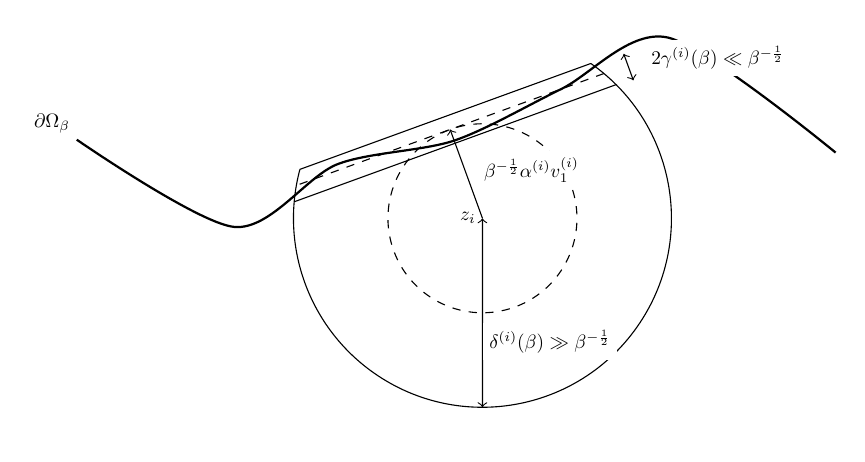
\begin{tikzpicture}[rotate = 20,scale=1.5, transform shape=false]

        %% paths
        \draw[black, thick] plot [smooth] coordinates {(0,-0.7) (1,-1.85) (2,-1.65) (3,-1.8) (4,-1.7) (5,-1.6) (6,-3)}; %boundary
        \draw[dashed] (3,-2.5) circle (0.8  ); %inner circle
        \draw (3,-2.5) ++(35:1.6) arc (35:-215:1.6); %outer arc
        \draw (3,-2.5) +(25:1.6) -- +(-205:1.6); % tangent segment
        \draw[dashed] (3,-2.5) +(30:1.6) -- +(-210:1.6); % tangent segment
        \draw (3,-2.5) +(35:1.6) -- +(-215:1.6); % tangent segment
        % arrows
        
        \draw[<->] (3,-2.5) +(0:0) -- +(-110:1.6);
        \draw[->] (3,-2.5) +(0:0) -- +(90:0.8);
        \draw[<->] (3,-2.5) +(1.6,0.66) -- +(1.6,0.9);
        
        % labels
        \draw (0,-0.7) node[above left,scale=0.7,fill=white] {$\partial \Omega_\beta$};
        \draw (3,-2.5) node[left,scale=0.7] {$z_i$};
        \draw (3,-2.5) +(1.7,0.66) node[above right,scale=0.7,fill=white] {$2\gammaPerturbation{i}(\beta)\ll \beta^{-\frac12}$};
        \draw (3.1,-2.5) +(90:0.4) node[right,scale=0.69,fill=white] {$\beta^{-\frac12}\epsLimit{i}\hessEigvec{i}{1}$};
        \draw (3,-2.5) +(-110:1.2) node[above right,scale=0.7,fill=white] {$\deltaRadius{i}(\beta)\gg \beta^{-\frac12}$};
    \end{tikzpicture}
        \caption{The local geometry of~$\Omega_\beta$ in the neighborhood of a critical point~$z_i$ which is close to the boundary.}
    \end{figure}

    % \todo[inline]{Dessins...}
    % The assumption that the~$\Omega_\beta$ are non-increasing implies that,~$\beta \mapsto \varepsilon^{(i)}(\beta)$ is also non-increasing for all~$i$ and~$\varepsiloni(\beta)<\deltai(\beta)$.
    % Geometrically, the neighborhoods~$\localNeighborhood{i}$ correspond to capped Euclidean balls, which have been cut by a hyperplane orthogonal the least contractive direction for the steepest descent flow around a the associated critical point, and thus 
    % We will use the following terminology to distinguish between different scalings 
    % Note that~$\left({\beta|\hessEigval{i}{1}|}\right)^{-\frac12}$ is the standard deviation of the local Gaussian approximation of~$\e^{\beta V}$ along the unstable manifold around a first-order saddle-point~$z_i$, which is given locally by the map~$\xi \mapsto \e^{\beta V(z_i + \xi \hessEigval{i}{1})}$. This is the motivation for the choice of scaling in the definition of~$\epsLimit{i}$. 
    
    % Let us make the further assumption that all critical points which are not order one saddle points are far from the boundary. In the case of the minimum~$z_0$, this is implied by the Morse assumption and the fact that~$\Omega_\beta$ contains~$\mathbf B$.

    % We then make the following further assumptions:
    % \begin{itemize}
    %     \item (coreset) There exists~$r>0$ such that \[\varepsilon_\beta^{(0)} > r.\]
    %     \item (spill out in unstable direction) In the (sub)critical case,~$\varepsilon_\beta^{(i)} \to 0$ as~$\beta\to\infty$. Denoting then by~$v_1^{(i)}$ an eigenvector of~$\nabla^2 V(z_i)$ associated with the unique negative eigenvalue, we assume that~$v_1^{(i)} \sim\mathrm{n}_{\partial\Omega_\beta}(x_\beta)$ in the sense of essential convergence, for any~$(x_\beta)_{\beta\geq 0}\in \prod_{\beta>0}\partial\Omega_\beta$ such that~$\varepsilon_\beta^{(i)} = |x_\beta-z^{(i)}|$.
    % \end{itemize}

    % It is helpful to think loosely of~$\Omega_\beta$ as a positive temperature perturbation of the bassin of attraction of~$z_0$ for the steepest-descent dynamics~$\dot X = - \nabla V(X)$.
    % We define
    %~$$ \lambda_{1,\beta} \leq \lambda_{2,\beta} \leq \dotsm~$$
    % the sequence of eigenvalues of~$-\cL_\beta$ on the domain~$H_0^1\cap H^2(\Omega_\beta; \mu) \subset L^2_\mu$, for which it is self-adjoint with pure point spectrum.

    \section{Limiting behavior of the low-lying spectrum}
    \label{sec:harm}
    We first aim to generalize the harmonic approximation of~\cite{S83} to the case of a temperature-dependent Dirichlet boundary condition, treating in particular the case in which the distance to the boundary scales critically with the temperature.
    We will show the following theorem:
    \begin{theorem}[Harmonic approximation]
        \label{thm:harm_approx}
        Assume that~,~\eqref{eq:epsLimit_definition},~\eqref{eq:domain_sandwich_inclusion} and~\eqref{eq:scaling_deltai} hold, and let~$k\geq 1$. Then the following holds:
        \begin{equation}
            \label{eq:harm_limit}
            \underset{\beta\to\infty}{\lim}\,\lambda_{k,\beta} = \lambda_{k,\alpha}^{\mathrm{H}},
        \end{equation}
        where~$\alpha$ is given by~\eqref{eq:global_alpha}, and~$\lambda_{k,\beta}$ is the~$k$-th Dirichlet eigenvalue of the operator~\eqref{eq:generator} in~$\Omega_\beta$.
    \end{theorem}
    In the above,~$\lambda_{k,\alpha}^{\mathrm H}$ denotes the~$k$-th eigenvalue of some temperature-independent operator defined in~Equation~\eqref{eq:global_harmonic_approximation_conj}, the harmonic approximation to the Witten Laplacian. The vector~$\alpha\in(-\infty,+\infty]^{1+m+r}$ encodes the asymptotic distance to the boundary of each critical points in the semiclassical scaling, and its~$i$-th component is given by the limit~$\epsLimit{i}$.
    The proof of Theorem~\ref{thm:harm_approx} relies on the construction of approximate eigenvectors for the Witten Laplacian, which are composed 

    \subsection{Definition of the harmonic approximation}
    This operator is obtained by considering local approximations around each critical point~$z_i$, which are harmonic oscillators whose realization depends on the value of the limit~$\epsLimit{i} \in [0,\infty]$.
    % \begin{definition}
    %     \label{def:model_spaces}
    %     \begin{itemize} 
    %         \item If~$z_i$ is supercritically close to the boundary:~$$S^{(i)} = (-\infty,0)\times \R^{d-1}.$$
    %         \item If~$z_i$ is critically close to the boundary:~$$ S^{(i)} = (-\infty,\alpha_i)\times \R^{d-1},\,\alpha_i = \frac{\alpha}{\sqrt{|\nu_1^{(i)}|}} >0.$$
    %         \item If~$z_i$ is far from the boundary:~$$S^{(i)} = \R^d.$$
    %     \end{itemize}
    % \end{definition}

    \subsection{Local harmonic models.\newline}\label{subsec:local_oscillators}
    The potential part of~$H_\beta = U_\beta - \Delta$, given by~$U_\beta=\frac12\left(\beta^2\frac{|\nabla V|^2}2-\beta\Delta V\right)$ is, at dominant order in~$\beta$, comprised of sharp wells centered around the critical points of~$V$. 
    The purpose of the harmonic approximation is to approximate~$H_\beta$ using independent local models consisting of shifted harmonic oscillators centered around each one of these wells, with frequencies prescribed by the eigenvalues of the~$\nabla^2 V$ at~$z_i$.
    Although very simple, this approximation is sufficient to capture the first-order behaviour of the bottom of the spectrum of~$-\cL_\beta$. 

    \[\Sigma^{(i)} = \frac12\Hess (\frac14|\nabla V|^2)(z_i)  = \frac12\left[\frac12 D^3 V \nabla V + \frac12 \left( \Hess V\right)^2 \right](z_i) = \frac14 \left(\Hess V\right)^2(z_i),\]
    and let
    \[\sigma(\Hess V(z_i)) = \{\nu_1^{(i)} \leq \nu_2^{(i)} \leq \dotsm \leq \nu_d^{(i)}\}\]
    denote the eigenvalues of~$\Hess V$ at~$z_i$, with
    \[U^{(i)} =\begin{pmatrix}v_1^{(i)}&\dotsm&v_d^{(i)}\end{pmatrix},\quad U^{(i)\intercal} \Sigma^{(i)} U^{(i)} = \frac14\mathrm{diag}\left[\left(\nu_j^{(i)}\right)^2,\,1\leq j\leq d\right] = \Lambda^{(i)}\]
    the associated orthonormal eigenbasis, which induces unitary transformation on flast $L^2$ spaces, via:
   ~$$ \mathcal U^{(i)} f(x) = f\left( U^{(i)\intercal}x\right),\quad \mathcal U^{(i)*} f(x) = f\left( U^{(i)}x\right).$$
    Since the critical points are non-degenerate,~$\nu_j^{(i)} \neq 0$ for all~$1\leq j\leq d,\,0\leq i \leq m+r$, and~$\nu_1^{i} < 0$ if and only if~$i\geq 1$.
    % Suppose~$z_i \in \partial \Omega$ for some~$i\geq 1$. In this case, assume that~$v_1^{(i)}$ is the outward normal to~$\Omega$ at~$z_i$,
    %  \todo[inline]{Preciser hypothese -- convergence de~$v_1^{(i)}$ vers~$\mathrm{n}_{\partial\Omega_\beta}(e_\beta(z^{(i)}))$ où~$|x-e_\beta(x)|=d(x,\partial\Omega_\beta)$ ("on dépasse dans la direction instable")} and introduce the half-space
    
    We define local harmonic approximations to~$H_\beta$ around each critical point:
    \[ H_\beta^{(i)} = -\Delta + \beta^2 (x-z_i)^\intercal \Sigma^{(i)}(x-z_i) - \beta \frac{\Delta V(z_i)}2, \]
    and the shifted harmonic oscillators:
    \[\Ki{} = -\Delta  + x^\intercal \Lambda^{(i)}x -\frac{\Delta V(z_i)}2.\]

    By dilation~$D_\lambda f(x) = \lambda^{d/2}f(\lambda x)$, translation~$T_b f(x) = f(x-b)$ and orthogonal change of coordinates~$\mathcal U^{(i)}$, a direct computation shows that
    the Dirichlet realization of~$H_{\beta}^{(i)}$ on~$L^2(\Omega_\beta)$ is unitarily equivalent to that of~$\beta \Ki{}$ on~$L^2(\sqrt{\beta}U^{(i)\intercal}(\Omega_\beta-z_i))$:
    \begin{equation}
        \label{eq:harmonic_conjugation}
        H_{\beta}^{(i)} = D_{\sqrt\beta}T_{\sqrt\beta z_i}\mathcal U^{(i)}\left(\beta \Ki{}\right)\mathcal U^{(i)*}T_{-\sqrt\beta z_i}D_{1/\sqrt\beta}.
    \end{equation}

    %~$$\mathbb H_{-}^{(i)} = \left\{ x \in \R^d\, \middle|\, x\cdot v_1^{(i)} < 0 \right\}.$$
    % \todo[inline]{Hypothese:~$\Omega \cap \left[ z_i + T_{z_i} \partial \Omega \right] = \{z_i\}$}

    \subsection{Harmonic eigenmodes.}
    In this section we define a family of self-adjoint realizations of the harmonic oscillators~$\Ki{}$, corresponding to various Dirichlet boundary conditions. These operators in turn will serve as local approximations of~$H_\beta$ around each critical point, allowing the construction of approximate eigenfunctions for~$H_\beta$ in the limit~$\beta\to\infty$.

    First, we recall classical results (see \cite{}) about the one-dimensional harmonic oscillator, and introduce some notation.
    The differential operator~$-\frac12\left(\partial_x^2-x^2\right)$ is essentially self-adjoint on~$\mathcal C_c^\infty(\R)$, and its closure, which we denote by~${\mathfrak H}_{\infty}$, has compact resolvent.
    We use the following notation for the eigendecomposition of~${\mathfrak H}_\infty$: for~$k\in\N$, we denote:
    \begin{equation}
        \label{eq:hermite_eigenfunction}
        w_{k,\infty}(x) = \frac{1}{\sqrt{2^k k! \sqrt\pi}}\e^{-\frac{x^2}2}H_k(x),
    \end{equation}
    where~$H_k$ is the~$k$-th Hermite polynomial. The function~$w_{k,\infty}$ is the~$k$-th eigenstate of~${\mathfrak H}_\infty$, with
    \begin{equation}
        \label{eq:hermite_eigenproblem}
         \mathfrak{H}_{\infty}w_{k,\infty} = \mu_{k,\infty} w_{k,\infty},\quad \mu_{k,\infty} = k + \frac12.
    \end{equation}

    The full harmonic oscillator will serve (after an appropriate change of scale), as a local approximation of~$H_\beta$ around critical points~$z_i$ which are far from the boundary, or to model the behaviour in the directions~$\hessEigvec{i}{j}$,~$2\leq j \leq d$ in the case where~$z_i$ is (super)critically close to the boundary.
    To construct a harmonic model for~$H_\beta$ around~$z_i$ critically close to the boundary in the direction~$\hessEigvec{i}{1}$, we must consider Dirichlet realizations of the harmonic oscillator, whose study is the object of the next paragraph.
    \subsection{Critical oscillators.}\label{subsec:critical_oscillators}
    In this paragraph, we introduce Dirichlet realizations for the harmonic oscillator which will serve as the basis for the construction of local models for~$H_\beta$ around critical points which are (super)critically close to the boundary.

    We consider the following dense subspace of~$L^2([a,b))$ for~$a<b\leq +\infty$:
    \[\mathcal C^\infty_{c,0}([a,b)) = \left\{f\in \mathcal C^\infty_c([a,b))\middle| f(a)=0\right\}.\]
    First we recall a few properties of the harmonic half-oscillator (see for instance the proof of~\cite[Proposition S1.2.10]{BS12}): the symmetric operator
   ~$$ \widetilde{\mathfrak H}_0 = -\frac12(\partial_x^2-x^2),\quad \mathcal D(\widetilde{\mathfrak H}_0) = \mathcal C^\infty_{c,0}([0,+\infty)),$$
    %~$$ \widetilde{\mathfrak H}_\infty = -\frac12(\partial_x^2-x^2),\quad \mathcal D(\widetilde{\mathfrak H}_\infty) = \mathcal C^\infty_{c}(\R)$$
    is essentially self-adjoint. Its unique self-adjoint extension, denoted~$\mathfrak{H}_0$, has the following spectral decomposition:
    \begin{equation}
        \label{harmonic_half_oscillator}
        \mathfrak{H}_0 w_{2k+1,\infty} = \left(2k + \frac32\right) w_{2k+1,\infty},\qquad k\in \N,
    \end{equation}
    where the family~$(\sqrt 2 w_{2k+1,\infty})_{k\geq 0}$ is an orthonormal eigenbasis for~$\mathfrak{H}_0$ (the~$\sqrt 2$ factor accounts for normalization in~$L^2$). Furthermore,~$\mathfrak{H}_0$ has compact resolvent, and the following inclusion holds:~$\mathcal D({\mathfrak{H}}_0) \subset H_0^1([0,+\infty))$.
    We aim to study, for~$\alpha\in\R$, the spectrum of a self-adjoint realization of the canonical oscillator~$-\frac12(\partial_x^2-\frac{x^2}2)$ with Dirichlet boundary conditions on~$[\alpha,+\infty)$, and in particular show that its spectrum is (essentially) composed of isolated eigenvalues of finite multiplicity which moreover depend analytically on~$\alpha$.
    To this end, we use a perturbative approach. Changing domains by translating positions with~$y = x-\alpha$, we see that the spectral properties of the operator:
   ~$$\widetilde{\mathfrak H}_\alpha = -\frac12(\partial_x^2-x^2),\quad \mathcal D(\widetilde{\mathfrak H}_\alpha) = \mathcal C^\infty_{c,0}([-\alpha,+\infty))$$
    can be deduced by those of the following operator:
   ~$$-\frac12(\partial_y^2-y^2) + \alpha y +\frac{\alpha^2}2 = \widetilde{\mathfrak H}_0 + V_\alpha + \frac{\alpha^2}2, \mathcal D(V_\alpha) = C^\infty_{c,0}([0,+\infty)).$$
    Since the constant~$\frac{\alpha^2}2$ only shifts the spectrum by a quantity which is analytic in~$\alpha$, it is enough to consider the operator:
   ~$$\widetilde{\mathfrak{G}}_\alpha = \widetilde{\mathfrak{H}}_0 + \alpha y.$$

    We first show that~$\widetilde{\mathfrak{G}}_\alpha$ is essentially self-adjoint.
    To show this, we first show that~$\alpha y$ is~$\widetilde{\mathfrak H}_0$-bounded with relative norm~$0$, computing, for~$\varphi \in \mathcal C^\infty_c([0,+\infty))$ and any~$M>0$:

    \begin{equation}
        \begin{aligned}
            \|\alpha y\varphi\|^2 &= \alpha^2\int_0^\infty y^2\varphi^2(y)\,\d y\\
            &\leq \alpha^2 M^2\int_0^M \varphi^2(y)\,\d y + \frac{\alpha^2}{M^2}\int_M^\infty y^4\varphi(y)^2\,\d y\\
            &\leq \alpha^2 M^2\|\varphi\|^2 + \frac{\alpha^2}{M^2}\|y^2\varphi\|^2\\
             &= \alpha^2M^2\|\varphi\|^2 + \frac{\alpha^2}{M^2}\left(4\|\widetilde{\mathfrak H}_0\varphi\|^2 +\int_0^\infty \left[2y^2 \varphi(y)\varphi''(y)-\varphi''(y)^2\right]\,\d y\right)\\
             &\leq \alpha^2 M^2\|\varphi\|^2 + \frac{4\alpha^2}{M^2}\|\widetilde{\mathfrak H}_0 \varphi\|^2 + \frac{2\alpha^2}{M^2}\int_0^\infty y^2 \varphi(y)\varphi''(y)\, d y\\
        \end{aligned}
    \end{equation}

    We may treat the remaining integral using two successive integration by parts, observing that at each step, the boundary term at zero vanishes since~$\varphi(0)=0$ is a factor:
    \begin{equation}
        \begin{aligned}
            \int_0^\infty y^2\varphi(y)\varphi''(y)\,\d y &= -\int_0^\infty (2y\varphi(y) + y^2 \varphi'(y))\varphi'(y)\,\d y\\
            & \leq -\int_0^\infty 2y\varphi(y)\varphi'(y)\, \d y\\
            &= \|\varphi\|^2.
        \end{aligned}
    \end{equation}

    It follows that
    \begin{equation}
        \label{eq:relative_bound}
        \|\alpha y \varphi\| \leq |\alpha|\sqrt{M^2+\frac{2}{M^2}}\|\varphi\| + \frac{2|\alpha|}M \| \widetilde{\mathfrak H}_0 \varphi\|,
    \end{equation}
    and the claim follows by taking~$M\to \infty$.

    Since~$\alpha y$ is~$\widetilde{\mathfrak H}_0$-bounded with relative norm 0, by the Kato--Rellich theorem~\cite[Theorem 6.4]{T14},~$\widetilde{\mathfrak{G}}_\alpha=\widetilde{\mathfrak H}_0 + \alpha y$ is essentially self-adjoint on~$\mathcal D({\widetilde{\mathfrak{H}}}_0)$, and its unique self-adjoint extension has domain
    \[\mathcal D(\mathfrak{G}_\alpha) = \mathcal D({\mathfrak{H}_0}),\]
    which is independent of~$\alpha$.
    We denote by~$\mathfrak{G}_\alpha$ the closure of~${\widetilde{\mathfrak{G}}}_\alpha$, and~$\mathfrak{H}_\alpha$ the corresponding self-adjoint operator on~$L^2([\alpha,+\infty))$ obtained by translating back to~$x=y+\alpha$ coordinates and appropriately shifting the spectrum by~$\alpha^2/2$.
    % We note that the same argument may be repeated to show that for any~$\alpha,\alpha'\in \R$,~$\mathfrak{G}_\alpha$ is~$\mathfrak{G}_{\alpha'}$-bounded with relative norm~$0$.
    Let us denote, for~$\lambda\not\in \sigma\left(\mathfrak{G}_\alpha\right)$, the resolvent:
    \[R_{\alpha}(\lambda) = \left(\mathfrak{G}_\alpha-\lambda\right)^{-1}.\]
    A straightforward consequence of the relative bound~\eqref{eq:relative_bound} (which extends to the closures of the operators at play) is that, for fixed~$\alpha\in \R$ and~$|\mathrm{Im}\,\lambda|$ sufficiently large,~$R_{\alpha}$ may be expanded into a normally convergent Dyson series:
    \begin{equation}
        \label{eq:dyson_expansion}
       R_{\alpha}(\lambda) = R_0(\lambda)\sum_{k=0}^\infty \alpha^k \left(y R_0(\lambda)\right)^k,
    \end{equation}
    which thus defines an analytic function of~$\alpha$. Furthermore, it is manifest from the expansion~\eqref{eq:dyson_expansion}, since~${\mathfrak H}_0$ has compact resolvent, that~$R_\alpha(\lambda)$ is compact, and hence~${\mathfrak G}_\alpha$,~${\mathfrak H}_\alpha$ also have compact resolvent. Since they are manifestly bounded below (by~$-\alpha^2/2$ and~$0$ respectively), their spectra are comprised of isolated eigenvalues of finite multiplicity tending to~$+\infty$.
    Standard results of perturbation theory~(see~\cite[Chapter VII]{K95}) apply. In particular, we get from~\eqref{eq:relative_bound} and~\cite[Theorem VII.2.6,Theorem VII.3.9]{K95} that~${\mathfrak G}_\alpha$ and thus~${\mathfrak H}_\alpha$ define self-adjoint holomorphic families of type (A) for~$\alpha\in\R$, and that there exists, for every~$k\in\N$, holomorphic functions~$\mu_{k,\alpha}$,~$w_{k,\alpha}$ satisfying the eigenrelation
    \begin{equation}
        \label{eq:holomorphic_eigensytem}
        {\mathfrak{H}}_\alpha w_{k,\alpha} = \mu_{k,\alpha} w_{k,\alpha},
    \end{equation}
    such that~$(v_{k,\alpha})_{k\in \N}$ is a dense orthonormal family in~$L^2([\alpha,+\infty))$. Moreover, the enumeration of these eigenpairs is fixed by the convention chosen for the harmonic half-oscillator, namely:
    \[v_{k,0} = \sqrt 2 v_{2k+1},\qquad \omega_{k,0} = 2k + \frac32.\]

    We highlight that we slightly abuse terminology when speaking of the holomorphic function~$\alpha\mapsto w_{k,\alpha}$, since these functions are, strictly speaking, elements of different Hilbert spaces. We will, here and thereafter, abuse notation and settle this issue by embedding them in~$L^2(\R)$ by extending them trivially by zero:
    \begin{equation}
        w_{k,\alpha}(x) = \1_{\alpha\leq x} w_{k,\alpha}(x),\quad x\in \R.
    \end{equation}

    \paragraph{The case~$d=1$.\newline}
    Using the change of variables~$z=\sqrt{\frac{|\nu_1^{(i)}|}2}x$, which gives~$\frac{\nu_1^{(i)2}}4 x^2-\partial_x^2 = |\nu_1^{(i)}|\frac12\left(z^2-\partial_z^2\right)$, we denote, for~$k\geq 0$ and~$\alpha\in [0,\infty]$:
    \begin{equation}
        \label{eq:hermite_eigenfunction_scaled}
        \wi{k}{\alpha}(x) = \left(\frac{|\nu_1^{(i)}|}{2}\right)^{\frac14}v_{k,-\alpha(|\hessEigval{i}{1}|/2)^{\frac12}}\left(-\sqrt{\frac{|\nu^{(i)}_1|}2}x\right) ,\qquad \omegai{k}{\alpha} = |\nu^{(i)}_1|\mu_{k,-\alpha(|\hessEigval{i}{1}|/2)^{\frac12}} - \frac{\nu^{(i)}_1}2.
    \end{equation}
    Note that that the sign of the variable has been flipped to conform with the orientation convention chosen for~$\hessEigvec{i}{1}$.
    It is immediate, from the construction performed above, that~$(\wi{k}{\alpha})_{k}$ forms a complete orthonormal eigenbasis for the Dirichlet realization of the oscillator~$\Ki{\alpha}$ on~$L^2((-\infty,\alpha))$, and hence~$\Ki{\alpha}$ is self-adjoint with domain:
        \begin{equation}
            \label{eq:full_oscillator_domain}
            D(\Ki{\alpha}) = \left\{ u \in L^2(\R):\quad \sum_{k=0}^\infty \left(\omegai{k}{\alpha}\right)^2\left|\left\langle u,\wi{k}{\alpha}\right\rangle\right|^2<+\infty\right\} \subset H_0^1(-\infty,\alpha).
        \end{equation}

    The higher dimensional case is simply obtained by tensorizing one-dimensional eigenmodes.

    % We are left to treat the case~$\alpha \geq 0$. To this end, we use a reflection trick. For a function~$f\in L^2(\R)$, we will use the notation 
    %~$$\iota_\alpha f(x) = f(2\alpha- x)$$
    % for the isometric involution reflecting~$f$ across~$\{x=\alpha\}$. 
    % We now consider the Schrödinger operator on~$L^2(\R)$ obtained by reflecting the potential term of~$K^{(i)}$ across~$\{x=\alpha\}$, and take its Friedrichs extension (we refer the reader to~\cite[Section X.3]{RS75} for background material on this topic), whose existence is guaranteed by the non-degenerancy of~$z_i$ which implies~$\nu_1^{(i)2}>0$.
    % Thus,~$\widetilde K^{(i)}_\alpha$ is the Friedrichs extension associated with the quadratic form of the following semi-bounded operator with domain~$\mathcal C^\infty_c(\R)$:
    %~$$-\Delta + W^{(i)}{\mathbbm 1}_{x\leq \alpha}+\iota_\alpha W^{(i)}{\mathbbm 1}_{x > \alpha} = - \Delta + \widetilde W^{(i)},$$ 
    % where the potential~$\widetilde W^{(i)}x = \frac{\nu_1^{(i)2}}4x^2-\frac{\nu_1^{(i)}}2$ is continuous.
    % Since~$-\frac{\nu_1^{(i)}}2\leq \widetilde W^{(i)}(x) \overset{|x|\to +\infty}{\longrightarrow}\, + \infty$, the operator~$\widetilde K^{(i)}_\alpha$ is self-adjoint with compact resolvent, by a classical result on Schrödinger operators,~\cite[Theorem XIII.67]{RS78}.
    % Thus, its spectrum is composed of isolated eigenvalues of finite multiplicity, tending to~$+\infty$. In fact, since~$-\Delta + \widetilde W^{(i)}$ is essentially self-adjoint on~$\mathcal C^\infty_c(\R)$ (see~\cite[Theorem 1.1]{BS12}), this extension is unique.
    
    % It is furthermore simple to check, by symmetry of the potential~$\widetilde W^{(i)}$, that the commutation~$\iota_\alpha\widetilde K^{(i),\alpha} = \widetilde K^{(i),\alpha}\iota_\alpha$ holds. 
    % Thus,~$\widetilde K^{(i)}_{\alpha}$ admits an eigendecomposition~$(\widetilde\lambda^{(i)}_{k,\alpha},\widetilde w^{(i)}_{k,\alpha})_{k\geq 0}$ such that~$\iota_\alpha\widetilde w^{(i)}_{k,\alpha} \in \{\pm \widetilde w^{(i)}_{k,\alpha}\}$ for all~$k\geq 0$.
    % Denote by~$(\lambda^{(i)}_{l,\alpha},w^{(i)}_{l,\alpha})_{l\geq 1}$ the restrictions of the (infinite) family of eigenpairs for which~$\iota_\alpha\widetilde w_{l,\alpha} = -\widetilde w_{l,\alpha}$ to the half-space~$(-\infty,\alpha)$. Since the~$(\widetilde w^{(i)}_{k,\alpha})_{k\geq 1}$ forms a complete orthonormal family of~$L^2(\R)$, so do~$( w^{(i)}_{l,\alpha})_{l\geq 1}$ for~$L^2(-\infty,\alpha)$, since any~$f\in L^2(-\infty,\alpha)$ may be obtained by restricting~$\widetilde f = f\mathbbm 1_{x<\alpha}-\iota_\alpha f \mathbbm 1_{x\geq \alpha}$ to the half-space, where~$\langle \widetilde f,\widetilde w^{(i)}_{k,\alpha}\rangle = 0$ for any~$k$ such that~$\iota_\alpha\widetilde w^{(i)}_{k,\alpha} = \widetilde w^{(i)}_{k,\alpha}$.
    
    % Similar to the oscillator on the full space, we define~$\Ki{\alpha}$ by its spectral decomposition:
    % \begin{equation}
    %     D(\Ki{\alpha}) = \left\{u\in L^2(-\infty,\alpha),\quad\sum_{l=0}^\infty \left(\omegai{l}{\alpha}\right)^2 \left|\left\langle u,\wi{l}{\alpha}\right\rangle\right|^2 < +\infty\right\},
    % \end{equation}
    % and let
    % \begin{equation}
    %     \Ki{\alpha} = \sum_{k=0}^\infty \omegai{k}{\alpha}\left\langle u ,\wi{k}{\alpha}\right\rangle \wi{k}{\alpha}\qquad\forall\, u\in D(\Ki{\alpha}).
    % \end{equation}

    % Here, we note that, in the case~$\alpha=0$, owing to the essential self-adjointness of~$-\partial_x^2 + \frac{\nu^{(i)2}_1}4 x^2$ on~$\mathcal C^\infty_c(\R)$, the reflected operator and the full harmonic oscillator coincide:~$\widetilde{K}^{(i)}_0 = K^{(i)}_\infty$, thus we recover the well-known property of the half-harmonic oscillator, whose eigenstates are given by the odd eigenstates of the full harmonic oscillator:
    % \begin{equation}
    %     \label{eq:half_harmonic_eigenstates}
    %     \wi{k}{0} = \sqrt2\wi{2k+1}{\infty}\mathbbm 1_{(-\infty,0)},\qquad \omegai{k}{0} = \omegai{2k+1}{\infty}.
    % \end{equation}
    % Here, we extend~$\wi{k}{0}$ by~$0$ outside its domain, and introduce a~$\sqrt2$ factor to account for~$L^2$ normalization.
    \paragraph{The case~$d\geq2$.\newline}
    We derive the general case by taking tensor products of the one-dimensional oscillators.
    Namely, we define, for~$n\in\N^d$:
    \begin{equation}
        \label{eq:full_harmonic_eigenstates}
        \lambdai{n}{\alpha} = \omegai{n_1}{\alpha} + \sum_{j=2}^{d}\left[|\nu_j^{(i)}|\mu_{n_j,\infty} - \frac{\nu_j^{(i)}}2\right],\qquad\psii{n}{\alpha}(x)= \wi{n_1}{\alpha}(x_1)\prod_{j=2}^d \left[\left(\frac{|\nu_j^{(i)}|}{2}\right)^{\frac14}w_{n_j,\infty}\left(\sqrt{\frac{|\nu^{(i)}_j|}2}x_j\right)\right],
    \end{equation}
    \begin{equation}
        \label{eq:full_harmonic_domain}
        D(\Ki{\alpha}) = \left\{u\in L^2\left[(-\infty,\alpha)\times\R^{d-1}\right],\quad\sum_{n\in\N^d}^\infty \left(\lambdai{n}{\alpha}\right)^2 \left|\left\langle u,\psii{n}{\alpha}\right\rangle\right|^2 < +\infty\right\}\subset H_0^1\left[(-\infty,\alpha)\times\R^{d-1}\right],
    \end{equation}
    \begin{equation}
        \label{eq:full_harmonic_expression}
        \Ki{\alpha}u = \sum_{n\in\N^d}^\infty \lambdai{n}{\alpha}\left\langle u ,\psii{n}{\alpha}\right\rangle \psii{n}{\alpha},\qquad \forall\, u\in D(\Ki{\alpha}).
    \end{equation}

    It is immediate from the construction performed above that~$\Ki{\alpha}$ is a self-adjoint on~$L^2((-\infty,\alpha)\times\R^{d-1})$, with compact resolvent, and a spectrum consisting of isolated eigenvalues of finite multiplicity tending to~$+\infty$.
    As before, we allow ourselves to consider each~$\psii{n}{\alpha}$ as an element of~$L^2(\R^d)$ by extending it by zero outside of~$(-\infty,\alpha)\times\R^{d-1}$.

    Furthermore, we have the following pointwise decay estimate for eigenmodes.
    \begin{lemma}
        For any~$n\in\N^d$ and~$\alpha\in(-\infty,\infty]$, there exists a constant~$C_{i,n,\alpha}>0$ such that the following inequality holds for almost every~$x$ in~$\R^d$:
        \begin{equation}
            \label{eq:exponential_decay}
            |\psii{n}{\alpha}(x)| \leq C_{i,n,\alpha}\,\e^{-\frac{|x|^2}{C_{i,n,\alpha}}}.
        \end{equation}
    \end{lemma}
    \begin{proof}
        The proof relies on a probabilistic estimate obtained in~\cite{C78}, and a reflection argument.
        We consider the following anti-symmetrization of the eigenmode~$\psii{n}{\alpha}$:
        \begin{equation}
            \widetilde{\psi}^{(i)}_{n,\alpha}(x) = \psii{n}{\alpha}(x)\1_{x\leq \alpha} - \psii{n}{\alpha}(\iota_\alpha x)\1_{x>\alpha},
        \end{equation}
        where~$\iota_\alpha(x) = (2\alpha-x,\dots,x_d)$ denotes the reflection with respect to the~$\{x_1 = \alpha\}$ hyperplane. Then, it is easy to check that~$\widetilde{\psi}^{(i)}_{n,\alpha}$
        is also an eigenmode (for the same eigenvalue~$\lambdai{n}{\alpha}$) of the Schr\"odinger operator associated with the symmetrized potential:
        \begin{equation}
            \widetilde K^{(i)}_\alpha = \widetilde W^{(i)} - \Delta,\quad \widetilde W^{(i)}(x) = W^{(i)}(x)\1_{x\leq \alpha} + W^{(i)}(\iota_\alpha x)\1_{x>\alpha},
        \end{equation}
        We note that there exists a compact set~$B_i\subset \R^d$, depending only on~$i$, and~$\varepsilon>0$ such that
        \begin{equation}
            \label{eq:lemma1_minorization}
            \widetilde W^{(i)} \geq \varepsilon|x|^2,\quad \forall\,x\in \R^d\setminus B_i,
        \end{equation}
        owing to the strict positivity of~$\Lambda^{(i)}$ (recalling that~$z_i$ is a non-degenerate critical point).
        We consider~$\widetilde K^{(i)}$ to be the self-adjoint extension of a formal operator defined as a Friedrichs extension of the lower-bounded quadratic form associated with~$K^{(i)}$.
        Then, it immediately follows from~\cite[Proposition 3.1]{C78} and the lower bound~\eqref{eq:lemma1_minorization} that the pointwise estimate~\eqref{eq:exponential_decay} holds for~$\widetilde\psi^{(i)}_{n,\alpha}$ and some constant~$C_{i,n,\alpha}$.
        The proof is concluded, since~$|\psii{n}{,\alpha}(x)|\leq |\widetilde\psi^{(i)}_{n,\alpha}(x)|$ for all~$x$.
    \end{proof}


    % \todo[inline]{la pire constante devrait être pour~$\alpha=0$, donnerait uniformité des estimées en~$\alpha$}

    % \begin{proof}
    %     % XIII.67 Reed-Simon, bug sur les domaines => passer par forme quadratique + Friedrich pour écrire le domaine
    %     % 2.10 Teschl
    %     The assumption that~$z_i$ is a non-degenerate critical point implies the case~$\alpha = +\infty$ by a standard result on Schrödinger operators,~\cite[Theorem XIII.67]{RS78}, as
    %    ~$$-\frac{\Delta V(z_i)}2\leq W^{(i)}(x) := x^\intercal \Lambda^{(i)}x - \frac{\Delta V(z_i)}2 \underset{|x|\to\infty}{\longrightarrow} +\infty.$$
    %     Thus, it is enough to treat the case~$\alpha\geq 0$.
        
    %     We start with the case$d = 1$. 
        
    %     Thus~$\sigma(\widetilde K^{(i),\alpha})$ consists of a sequence of isolated eigenvalues of finite multiplicity tending to~$+\infty$.

    %     % The claim is implied by the inclusion~$\sigma(K^{(i)}) \subset \sigma(\widetilde K^{(i)})$, which is equivalent to the reverse inclusion of resolvent sets.
    %     % Let~$\lambda\in  \mathbb C \setminus \sigma(\widetilde K^{(i)})$, and~$f\in L^{2}(S^{(i)})$. We define~$\widetilde u \in H^2(\R)$ as the~$\lambda$-resolvent of~$\widetilde K^{(i)}$ applied to the odd reflection of~$f$ along~$\partial S^{(i)}$:
    %     %~$$\widetilde f(x) = f{\mathbbm 1}_{x\leq \alpha} - \iota_\alpha f{\mathbbm 1}_{x>\alpha},\qquad (\lambda-\widetilde K^{(i)}) \widetilde u = \widetilde f,\qquad \|\widetilde u\|_{L^2(\R)}\leq C_\lambda \|\widetilde f\|_{L^2(\R)},$$
    %     % for some~$C_\lambda>0$ independent of~$f$.
     
    %     It remains to show that~$\psi_l \in D(K^{(i),\alpha})$. By definition of the Friedrichs extension, this is given by the closure of~$\mathcal C_c^\infty((-\infty,\alpha))$ under the norm:
    %     \[\|u\|_{K^{(i),\alpha}} = \left\langle K^{(i),\alpha} u ,u\right\rangle + \left(1+\frac{\Delta V(z_i)}2\right)\|u\|_{L^2(-\infty,\alpha)}.\]
    %     However, note that~$\psi_l$ is given by the restriction of an element of~$\mathrm{Ker}\,(\iota_\alpha-1)$ to the half-space, and that~$\iota_\alpha$ is continuous for the norm
    %     \[\|u\|_{\widetilde K^{(i),\alpha}} = \left\langle \widetilde K^{(i),\alpha} u ,u\right\rangle + \left(1+\frac{\Delta V(z_i)}2\right)\|u\|_{L^2(\R)}.\]
    %     Thus,~$\widetilde\psi_l$ may be written 
    %     The case~$d\geq 1$ then easily follows, since one can write a complete orthonormal eigenbasis for~$K^{(i),\alpha}$, which may constructed by taking the tensor product of the eigenbases for each of the one-dimensional oscillators
    %     \[-\partial_{x_j}^2 + \frac{\nu_j^{(i)2}}4x_j^2,\quad 1\leq j\leq d.\]

    %     The pointwise decay estimate~\eqref{eq:exponential_decay} is settled for the cases~$\alpha=0$ and~$\alpha=+\infty$ by explicit expressions for the eigenfunctions (see ... below). The case~$\alpha>0$ is as a consequence of general pointwise bounds for Schrödinger eigenfunctions, see for instance the result~\cite[Proposition 3.1]{C78} from Carmona.
    % \end{proof}

    % Before giving explicit formulas for the spectral decomposition of~$K^{(i)}$
    % More explicitely, the spectrum of~$K^{(i),\alpha}$ is given by
    % \begin{equation}
    %     \label{eq:harmonic_spectrum}
    %     \sigma(K^{(i),\alpha}) = \left(\frac12\left[\sum_{j=1}^d |\nu_j^{(i)}|(2n_j+1)-\nu_j^{(i)}\right],\quad n\in\N^d\right)
    % \end{equation}

    % \paragraph{The supercritical case~$S^{(i)} = \R^d$.\newline}
    % In this case, the spectrum is given by
    % \[.\]
    % For~$i=0$,~$\nu_j^{(i)} = |\nu_j^{(i)}|$, hence
    % \[\sigma(K^{(0)}) = \left\{\sum_{j=1}^d \nu_j^{(i)}n_j,\quad n\in\N^d\right\}\ni 0.\]
    % For~$i\geq 1$,~$\nu_1^{(i)} = -|\nu_1^{(i)}|$ and~$\nu_j^{(i)} = |\nu_j^{(i)}|,\, j \geq 2$, thus
    % \[\sigma(K^{(i)}) = \left\{|\nu_1^{(i)}|(n_1+1)+\sum_{j=2}^d \nu_j^{(i)}n_j,\quad n\in\N^d\right\},\quad i \geq 1.\]
    % The bottom of the latter spectrum is given by~$|\nu_1^{(i)}|$. For simplicity, we will enumerate the eigenvalues using the following convention. For a multi-index~$n\in \N^d$,
    %~$$\nu_n^{(i)} = \sum_{j=1}^d |\nu_{j}^{(i)}|n_j + \mathbbm 1_{\nu_1^{(i)}<0}|\nu_1^{(i)}|,$$
    % and~$\psi^{(i)}_n$ the corresponding eigenfunction (which, up to a phase, we assume to be real-valued). Then,~$\psi^{(i)}_n$ has the following product form
    % \begin{equation}
    %     \label{eq:harmonic_eigenstates}
    %     \psi^{(i)}_n(x) = \prod_{j=1}^d  \left(\frac{|\nu_j^{(i)}|}{2}\right)^{\frac14}\psi_{n_j}\left(\sqrt{\frac{|\nu^{(i)}_j|}2}x_j\right)
    % \end{equation}
    % into a product of elementary eigenfunctions, where 
    
    % \paragraph{The subcritical case~$S^{(i)} = (-\infty,0)\times \R^{d-1}$.\newline}
    % The difference in this case is that the oscillator corresponding to the unstable direction is restricted to the half-space~$(-\infty,0)$. Its eigenstates correspond to the odd eigenstates of the harmonic oscillator on the full space. The spectrum is thus given, for~$i\geq 1$, by
    % \[\sigma(K^{(i)}) = \left\{|\nu_1^{(i)}|(2n_1+2)+\sum_{j=2}^d \nu_j^{(i)}n_j,\quad n\in\N^d\right\}\]
    % In this case, the bottom of the spectrum is given by
    %~$$2|\nu_1^{(i)}|.$$

    % The eigenfunctions have the same product form as \eqref{eq:harmonic_eigenstates}, but are restricted to the half-space, and only the odd modes contribute in the~$x_1$ direction. The factor~$\sqrt 2$ accounts for~$L^2$ normalization.

    % \begin{equation}
    %     \label{eq:harmonic_eigenstates_half_space}
    %     \psi^{(i)}_n(x) = \mathbbm{1}_{S^{(i)}}(x)\sqrt 2\left(\frac{|\nu_1^{(i)}|}{2}\right)^{\frac14}\psi_{2n_1+1}\left(\sqrt{\frac{|\nu^{(i)}_1|}2}x_1\right)\prod_{j=2}^d  \left(\frac{|\nu_j^{(i)}|}{2}\right)^{\frac14}\psi_{n_j}\left(\sqrt{\frac{|\nu^{(i)}_j|}2}x_j\right)
    % \end{equation}

    % \paragraph{The critical case~$S^{(i)} = (-\infty,\alpha_i) \times \R^{d-1}$.\newline}
    %     In this case, the spectrum of the oscillator corresponding to the unstable direction, restricted to the half-space~$(-\infty,\alpha_i)$, is not analytically known.

    %     Nevertheless, we denote for~$k\in\N$
    %    ~$$(\lambda_k^{\alpha},\psi_k^{\alpha})$$
    %     the~$k$-th~$L^2(S^{(i)})$-normalized eigenpair for the Dirichlet realization of the harmonic oscillator~$\frac12\left(x^2-\partial^2\right)$ on~$(-\infty,\alpha/\sqrt 2)$.
    %     \todo[inline]{A double-check..}
    %     The spectrum is then given, for~$i\geq 1$, by
    %    ~$$\sigma(K^{(i)}) = \left\{ |\nu_1^{(i)}|(\lambda_{n_1}^{\alpha} + \frac12) + \sum_{j=2}^d \nu_j^{(i)}n_j,\quad n\in\N^d\right\},$$
    %     the lowest eigenvalue is
    %    ~$$|\nu_1^{(i)}|\left(\lambda_{1}^{\alpha}+\frac12\right),$$
    %     and the eigenstates are given by
    %    ~$$\psi^{(i)}_n(x) = \mathbbm{1}_{S^{(i)}}(x)\left(\frac{|\nu_1^{(i)}|}{2}\right)^{\frac14}\psi_{n_j}^{\alpha}\left(\sqrt{\frac{|\nu^{(i)}_1|}2}x_1\right)\prod_{j=2}^d  \left(\frac{|\nu_j^{(i)}|}{2}\right)^{\frac14}\psi_{n_j}\left(\sqrt{\frac{|\nu^{(i)}_j|}2}x_j\right).$$
    % In each of the three cases, we denote by~$\lambda_k^{(i)}$ the~$k$-th eigenvalue of~$K^{(i)}$ acting on~$S^{(i)}$. In the case of an eigenvalue~$\lambda$ which occurs multiple times (that is, such that multiple~$d$-uplets~$n\in\N^d$ correspond to~$\lambda$), we convene that we count~$\lambda$ with multiplicity, using the enumeration induced by the lexicographic order on~$\N^d$. 

    \subsection{Global harmonic approximation.\newline}\label{subsec:global_harm_operator}
    We now define the global harmonic approximation to~$H_\beta$, associated with a vector of extended real numbers~$\alpha' = (\alpha'_0,\dots,\alpha'_{m+r}) \in (-\infty,\infty]^{1+m+r}$ encoding the Dirichlet boundary conditions.
    Recall, that for each~$i=0,\dotsm,m+r$, the extended real number~$\alpha_i$ is defined as the limit~$\underset{\beta\to\infty}{\lim}\,\sqrt\beta \varepsiloni(\beta)$, and so we also denote for convenience:
    \begin{equation}
        \label{eq:global_alpha}
        \alpha = \left(\alpha_i\right)_{i=0,\dots,m+r}.
    \end{equation}
    
    We define, for general~$\alpha'$, local oscillators~$H^{(i)}_{\beta,\alpha'_i}$ from the definition~$\Ki{\alpha'_i}$ using the unitary equivalence~\eqref{eq:harmonic_conjugation}. In particular, the domain of~$H_{\beta,\alpha'_i}^{(i)}$ is given by
    \begin{equation}
        \label{eq:local_harm_domain}
        D(H^{(i)}_{\beta,\alpha'_i}) = \left\{ u \in L^2\left[z_i + \halfSpace{i}\left(\frac{\alpha'_i}{\sqrt\beta}\right)\right],\quad  \mathcal U^{(i)*}T_{-\sqrt\beta z_i}D_{1/\sqrt\beta}u\in D(\Ki{\alpha'_i})\right\}.
    \end{equation}
    We denote by
    \begin{equation}
        \label{eq:harmonic_eigenmode}
        \psii{\beta,k}{\alpha_i'}(x) = \beta^{\frac14}\psii{k}{\alpha_i'}(\sqrt\beta U^{(i)\intercal}(x-z_i)),
    \end{equation}
    the eigenmode of~$H^{(i)}_{\beta,\alpha_i'}$ with eigenvalue~$\beta\lambdai_{k,\alpha_i'}$ associated with~$\psii{k}{\alpha_i'}$ under this correspondence. Note the~$\beta^{\frac14}$ factor, which accounts for~$L^2$ normalization.

    The global approximation is formed by a direct sum of these local oscillators:
    \begin{equation}
        \label{eq:global_harmonic_approximation_conj}
        H_{\beta,\alpha'}^{\mathrm H} = \bigoplus_{i=0}^{m+r} H^{(i)}_{\beta,\alpha'_i},\qquad D(H_{\beta,\alpha'}^{\mathrm H}) = \prod_{i=0}^{m+r} D(H^{(i)}_{\beta,\alpha'_i}),
    \end{equation}
    whence the harmonic spectrum is given by
    \begin{equation}
        \label{eq:full_harmonic_approximation_spectrum}
        \sigma(H_{\beta,\alpha'}^{\mathrm H}) = \left(\beta\lambdai{n}{\alpha'_i}\right)_{\substack{0\leq i\leq m+r\\n\in\N^d}}.
    \end{equation}
    
    For convenience, we specify the conventions we use to enumerate the various spectra at play.
    First, we enumerate the spectrum of~$\Ki{\alpha_i'}$ in non-decreasing order, defering to the lexicographic ordering on~$\N^d$ to resolve ambiguities from degenerate eigenvalues. Thus we have a non-decreasing family~$(\lambdai{n}{\alpha})_{n\in\N}$, and corresponding eigenmodes~$(\psii{n}{\alpha})_{n\in\N}$.
    We then enumerate the full harmonic spectrum in non-decreasing order, by defining two integer-valued sequences
    \begin{equation}
        \label{eq:eigenstate_enumeration}
        (k_j)_{j\geq 1}\in \N^{\N^*},\quad (i_j)_{k\geq 1}\in \{0,\dots,m+r\}^{\N^*},
    \end{equation}
    defined by the condition that the~$k$-th largest eigenvalue of~$H_\beta^{\mathrm H}$, counted with multiplicity, is given by:
    \begin{equation}
        \beta\lambda_{k,\alpha'}^{\mathrm H} = \beta\lambda^{(i_k)}_{n_k,\alpha'_{i_k}},
    \end{equation}
    where we first defer to the ordering on~$\{0,\dots,m+r\}$ and then to the ordering on each~$\sigma(\Ki{\alpha_i'})$ to resolve ambiguities from degenerate eigenvalues.

    For convenience, we also define, for each~$0\leq i \leq m+r$, the function which gives, for a given~$k\geq 1$, the number of eigenmodes corresponding to energy levels below~$\lambda_{\alpha'}^{\mathrm H}$ localized around~$z_i$:
    \begin{equation}
        \label{eq:def_ni}
        N_{i}(k) = \#\{ 1 \leq j \leq k: i_j = i\}.
    \end{equation}

    For simplicity, we have omitted to notate the dependence of~$N_i$,~$i_k$ and~$n_k$ in~$\alpha'$, which will be clear from the context.
    We also note the following obvious relations, valid for any~$k\geq 0$:
    \begin{equation}
        \label{eq:enumeration_relations}
        \underset{0\leq i\leq m+r}{\max}\,\lambda^{(i)}_{N_i(k),\alpha_i'}  = \lambda_{k,\alpha'}^{\mathrm H},\qquad \underset{0\leq i\leq m+r}{\min}\,\lambda^{(i)}_{N_i(k)+1,\alpha_i'} = \lambda_{k+1,\alpha'}^{\mathrm H},\qquad \sum_{i=0}^{m+r} N_i(k) = k.
    \end{equation}

    We highlight that the analyticity of the map~$\alpha \mapsto \mu_{k,\alpha}$ for all~$k\in \N$ implies that the map:
    \begin{equation}
        \label{eq:eigval_continuity}
        \alpha' \mapsto \lambda_{k,\alpha'}^{\mathrm H}
    \end{equation}
    is continuous.
    \subsection{Harmonic quasimodes.}\label{subsec:quasimodes}
    Approximate eigenmodes of~$H_\beta$ may be obtained by localizing the eigenmodes of the harmonic approximation around the corresponding critical point, in such a way that the Dirichlet boundary conditions in~$\Omega_\beta$ are met.
    We will consider so-called quasimodes of the form
    \begin{equation}
        \label{eq:harm_quasimode}
        \widetilde\psi^{(i)}_{\beta,k,\alpha} = \frac{\chi_\beta^{(i)}\psi_{\beta,k,\alpha}^{(i)}}{\|\chi_\beta^{(i)}\psi_{\beta,k,\alpha}^{(i)}\|_{L^2(\Omega_\beta)}},
    \end{equation}
    where~$\psi_{\beta,k,\alpha}^{(i)}$ is a harmonic mode of~$H_\beta^{(i),\alpha}$, multiplied by the cutoff function~$\chi_\beta^{(i)}$, and normalized in~$L^2(\Omega_\beta)$.
    The role of~$\chi_\beta^{(i)}$ is to localize the quasimode in the vicinity of~$z_i$, and ensure that the boundary conditions are met. To this effect, we fix a reference~$\mathcal C_c^\infty~$ cutoff function~$\chi$ such that
    \[\chi|_{B\left(0,\frac12\right)}\equiv 1,\quad \chi|_{\R^d\setminus B(0,1)} \equiv 0.\]
    We will furthermore require the following technical condition:
    \begin{equation}
        \label{eq:partition_of_unity_condition}
        \|\nabla\sqrt{1-\chi^2}\|_\infty < +\infty,
    \end{equation}
    which may be easily enforced by choosing~$\chi$ such that~$\chi \widesim{a^+} \mathrm{exp}\left(-\frac1{x-a}\right)$,~$\chi\widesim{b^-}\mathrm{exp}\left(-\frac1{b-x}\right)$, say for~$\supp\,\chi = [a,b]$.
    Let us next define the localized cutoff function:
    \begin{equation}
        \label{eq:cutoff}
        \chi_\beta^{(i)}(x) = \chi(\deltai(\beta)^{-1}|x-z_i|).
    \end{equation}
    Recalling that~$\sqrt\beta\deltai(\beta)\overset{\beta\to\infty}{\longrightarrow} + \infty$, we have that~$\supp \chi_\beta^{(i)}$ is contained in a small ball around~$z_i$, but which is large with respect to~$\frac1{\sqrt\beta}$, and~$\supp\,\nabla \chi_\beta^{(i)}$ is contained in a hyperspherical shell around~$z_i$:
    \begin{equation}
        \label{eq:cutoff_supports}
        \supp\,\chi_\beta^{(i)} \subset B(z_i,\deltai(\beta)),\quad\supp\,\nabla\chi_\beta^{(i)} \subset B(z_i,\deltai(\beta))\setminus B\left(z_i,\frac12\deltai(\beta)\right).
    \end{equation}

    In particular we have
    \begin{equation}
        \label{eq:linf_bound_nabla_chi}
        \|\partial^\alpha\chi_\beta^{(i)}\|_\infty = \|\partial^\alpha \chi\|_\infty \deltai(\beta)^{|\alpha|},
    \end{equation}
    for any multi-index~$\alpha$, hence~$\|\partial^\alpha \chi_\beta^{(i)}\|_\infty = \o(\beta^{\frac{|\alpha|}2})$ for~$|\alpha|\leq 2$.
    
    We stress that, although~$\chi_\beta^{(i)}$ does not itself vanish on~$\partial \Omega_\beta$ in general in the case where~$z_i$ is (super)critically close to the boundary, we still have
   ~$\widetilde\psi_{\beta,k,\alpha}^{(i)}\in H_0^1\cap H^2(\Omega_\beta)$ provided the harmonic eigenmode~$\psi_{\beta,k,\alpha}^{(i)}$ vanishes on~$C_i(\beta)$, where we recall the definition~\eqref{eq:def_ball_cap} of the spherical cap associated with~$z_i$.
    
    In the following lemma, we record some localization estimates.
    \begin{lemma}[Localization estimates]
        \label{lemma:localization}
        We consider normalized eigenvectors~$\psi_{\beta,n,\alpha}^{(i)}$ and~$\psi_{\beta,m,\alpha}^{(i)}$ of~$H^{(i)}_{\beta,\alpha}$ in~$L^2\left(\halfSpace{i}(\frac{\alpha}{\sqrt\beta})\right)$, and we define the associated quasimodes~$\widetilde\psi_{\beta,n,\alpha}^{(i)}$ and~$\widetilde\psi_{\beta,m,\alpha}^{(i)}$ according to the formula~\eqref{eq:harm_quasimode}.
        Then, there exists~$\beta_0>0$ and constants~$C_{n,i,\alpha},C_{m,i,\alpha},C_{n,m,i,\alpha}>0$, independent of~$\beta$ such that the following estimates hold for any~$\beta>\beta_0$.
        \begin{enumerate}[]
            \item{\begin{equation}\label{eq:loc_eqa}\|(1-\chi_\beta^{(i)})\psi_{\beta,n}^{(i)}\|_{L^2(\R^d)} \leq \frac{C_{n,i,\alpha}}{\beta^{\frac14}\deltai(\beta)^{\frac12}}\e^{-\frac{\beta\deltai(\beta)^2}{C_{n,i,\alpha}}},\end{equation}}
            \item{\begin{equation}\label{eq:loc_eqb}\left|\langle \widetilde\psi_{\beta,n}^{(i)},\widetilde\psi_{\beta,m}^{(i)}\rangle-\delta_{nm}\right| \leq  \frac{C_{n,m,i,\alpha}}{\beta^{\frac14}\deltai(\beta)^{\frac12}}\e^{-\frac{\beta\deltai(\beta)^2}{C_{n,m,i,\alpha}}},\end{equation}}
            \item{\begin{equation}\label{eq:loc_eqc}\left|\left\langle H_\beta^{(i)}(1-\chi_\beta^{(i)})\psi_{\beta,n}^{(i)},(1-\chi_\beta^{(i)})\psi_{\beta,m}^{(i)}\right\rangle_{L^2(\R^d)}\right|\leq \frac{C_{n,m,i,\alpha}}{\beta^{\frac12}\deltai(\beta)^{3}}\e^{-\frac{\beta\deltai(\beta)^2}{C_{n,m,i,\alpha}}}.\end{equation}}
        \end{enumerate}
        
        Furthermore, assuming~\eqref{eq:scaling_deltai}, these bounds decay faster than any polynomial growth in~$\beta$.
    \end{lemma}
    \begin{proof}
        We begin by proving~\eqref{eq:loc_eqa}.
        Changing coordinates with~$y = \sqrt\beta U^{(i)\intercal}(x-z_i)$, we get:
        \begin{equation}
            \begin{aligned}
                \|(1-\chi_\beta^{(i)})\psi_{\beta,n,\alpha}^{(i)}\|^2_{L^2(\R^d)} &= \int_{\R^d}\left(1-\chi\right)\left(\frac1{\sqrt\beta\deltai(\beta)}U^{(i)}y\right)\psi^{(i)}_{n,\alpha}(y)^2\,\d y\\
                &\leq \int_{\R^d\setminus B(0,\frac12 \sqrt\beta\deltai(\beta)}\psi^{(i)}_{n,\alpha}(y)^2\,\d y\\
                &\leq |\mathbb S^{d-1}|C_{n,i,\alpha}\int_{\frac12 \sqrt\beta\deltai(\beta)}^\infty\,s^{d-1}\e^{-\frac{s^2}{C_{n,i,\alpha}}}\,\d s,\\
                &\leq C'_{n,i,\alpha}\int_{\frac12 \sqrt\beta\deltai(\beta)}^\infty\,\e^{-\frac{s^2}{C'_{n,i,\alpha}}}\,\d s,
            \end{aligned}
        \end{equation}
        where we used respectively the condition~\eqref{eq:cutoff_supports} and the pointwise exponential decay estimate~\eqref{eq:exponential_decay} to obtain the first and second inequalities. Applying the standard Gaussian tail bound~$\int_t^\infty \e^{-s^2/2}\,\d s \leq t^{-1}\e^{-t^2/2}$ yields the desired bound~\eqref{eq:loc_eqa} upon taking~$C'_{n,i,\alpha}$ as large as necessary.

        To show~\eqref{eq:loc_eqb}, we first note that, since
       ~$\|\psi^{(i)}_{\beta,n,\alpha}\| =1$, and~$0\leq \chi_\beta^{(i)}\leq 1$, we obtain, by a simple triangle inequality:
        \[0\leq 1-\|\chi_\beta^{(i)}\psi^{(i)}_{\beta,n,\alpha}\|\leq \|(1-\chi_\beta^{(i)})\psi^{(i)}_{\beta,n,\alpha}\|,\]
        and thus
        \begin{equation}
            \label{eq:lemme2_normalization}
            1\leq \frac1{\|\chi_\beta^{(i)}\psi^{(i)}_{\beta,n,\alpha}\|} \leq 1 + 2\|(1-\chi_\beta^{(i)})\psi^{(i)}_{\beta,n,\alpha}\|
        \end{equation}
        for~$\beta$ sufficiently large. A similar estimate holds for~$\psi^{(i)}_{\beta,m,i}$.

        For convenience, we denote~$\psi^{(i)}_{\beta,n,\alpha} = \psi_n$,~$\psi^{(i)}_{\beta,m,\alpha}=\psi_m$ and~$\chi_\beta^{(i)}=\chi$. Then:
        \[\langle \chi \psi_n,\chi \psi_m\rangle = \langle \psi_n,\psi_m\rangle - 2\langle \psi_n,(1-\chi)\psi_m\rangle + \langle\psi_n,(1-\chi)^2\psi_m\rangle.\]
        Thus, by Cauchy--Schwarz inequalities, and using the orthogonality of~$\psi_n$ and~$\psi_m$, we obtain:
       \[ \left|\langle \chi\psi_n,\chi\psi_m\rangle - \delta_{n,m}\right| \leq 2 \|\psi_n\|\|(1-\chi)\psi_m\| + \|\psi_n\|\|(1-\chi)^2\psi_m\| \leq 3\|(1-\chi)\psi_m\|,\]
       since~$(1-\chi)^2\leq (1-\chi)$.
        
       Denoting~$\widetilde \psi_n = \chi\psi_n\|\chi\psi_n\|^{-1}, \widetilde \psi_m = \chi\psi_m\|\chi\psi_m\|^{-1}$, we deduce from~\eqref{eq:lemme2_normalization} that
       there exists constants~$C,\beta_0>0$ such that 
       \[\left|\langle \widetilde \psi_n,\widetilde \psi_m\rangle -\delta_{nm}\right|\leq \left|1-\frac{1}{\|\chi\psi_n\|\|\chi\psi_m\|}\right|\|\chi\psi_n\|\|\chi\psi_m\|\leq C(\|(1-\chi)\psi_m\| + \|(1-\chi)\psi_n\|)\]
       for all~$\beta>\beta_0$. Using the estimate~\eqref{eq:loc_eqa} then yields~\eqref{eq:loc_eqb}.

        For~\eqref{eq:loc_eqc}, we start with a small computation for a Schrödinger operator~$H = V-\Delta$ with domain~$D(H)\subset H^1(\R^d)$, two eigenstates~$u,v$ with respective eigenvalues~$\lambda_u,\lambda_v$, and~$\eta\in\mathcal C_c^\infty(\R^d)$.
        Using the relation
        \[H(\eta u) = \eta H u - 2\nabla \eta\cdot \nabla u - u \Delta \eta = \lambda_u \eta u - 2 \nabla \eta \cdot \nabla u  - u \Delta \eta,\]
        we get by integrating against~$\eta v$:
            \begin{align*}
                \langle H\eta u,\eta v\rangle = \lambda_u\langle u,\eta v\eta\rangle - \langle uv,\eta\Delta\eta\rangle -2 \langle v\nabla u,\eta\nabla\eta\rangle.
            \end{align*}
            Thus, by symmetry and an integration by parts, we get
            \begin{equation}
                \label{eq:energy_localization_formula}
                \langle H\eta u,\eta v\rangle = \langle uv,\frac{\lambda_u+\lambda_v}2\eta^2-\eta\Delta\eta\rangle -\langle \nabla[uv],\nabla[\eta^2]\rangle = \langle uv,\frac{\lambda_u+\lambda_v}2\eta^2+\eta\Delta\eta + 2|\nabla\eta|^2\rangle.
            \end{equation}
        
        Applying equation~\eqref{eq:energy_localization_formula} to~$H = H_{\beta,\alpha}^{(i)}$ with~$\eta = (1-\chi_\beta^{(i)})$, we get, noting that the test function~$\frac{\lambda_u+\lambda_v}2\eta^2+\eta\Delta\eta + 2|\nabla\eta|^2$ is supported in:
        \[\R^d\setminus B\left(z_i,\frac12\sqrt\beta\deltai(\beta)\right),\]
        \[\left\|\frac{\lambda_n+\lambda_m}{2}(1-\chi_\beta^{(i)})^2+(1-\chi_\beta^{(i)})\Delta(1-\chi_\beta^{(i)}) + 2|\nabla(1-\chi_\beta^{(i)})|^2\right\|_{\infty}\leq \frac{C_{n,m}}{\deltai(\beta)^2},\]
        using the crude estimate~\eqref{eq:linf_bound_nabla_chi}, whereby, using again the pointwise exponential decay of both~$\varphi$ and~$\psi$, and the same Gaussian tail estimate as for~\eqref{eq:loc_eqa}, we get, for some~$C>0$,
        \begin{equation}
            \begin{aligned}
                \left|\left\langle H_\beta^{(i)}(1-\chi_\beta^{(i)})\varphi_\beta^{(i)},(1-\chi_\beta^{(i)})\varphi_\beta^{(i)}\right\rangle \right| &\leq \frac{C}{\deltai(\beta)^2}\int_{\frac12\sqrt\beta\deltai(\beta)}^{+\infty}\,\e^{-\frac{2s^2}{C}}\,\d s\leq C\frac{\e^{-\frac{\beta\deltai(\beta)^2}{C}}}{\beta^{\frac12}\delta^{(i)}(\beta)^3}.
            \end{aligned}
        \end{equation}

        Finally, each of the bounds may be written in the form~$\frac{P(\beta)}{Q(T(\beta))}\e^{-cT(\beta)^2}$, where $T(\beta) = \sqrt\beta \delta^{(i)}(\beta)$ and $P,Q$ are polynomials. Since, under Assumption~\eqref{eq:scaling_deltai},~$T(\beta)$ goes to~$+\infty$ faster than~$\sqrt{\log\beta}$, we also have~$\frac{R(\beta)P(\beta)}{Q(T(\beta))}\e^{-cT(\beta)^2}\to 0$ for any polynomial~$R$.
    \end{proof}

    The following lemma justifies the local approximation of~$H_\beta$ by~$H_\beta^{(i)}$ around~$z_i$.
    \begin{lemma}[Taylor estimate]
        \label{lemma:taylor_bound}
        Fix~$0\leq i \leq m+r$ and~$u\in L^2(\Omega_\beta)$, and assume~\eqref{eq:deltai_polybound_close},~\eqref{eq:deltai_polybound_far} hold.
        There exists~$C>0$ and~$\beta_0>0$ such that, for all~$\beta>\beta_0$, the following estimate holds:
        \begin{equation}
            \label{eq:taylor_bound_witten}
            \|(H_\beta-H_\beta^{(i)})\chi_\beta^{(i)} u\| \leq C\beta^{3\scalingExp+\frac12}\|\chi_\beta^{(i)}u\| = \o(\beta)\|\chi_\beta^{(i)}u\|.
        \end{equation}
    \end{lemma}
    \begin{proof}
        Since~$H_\beta-H_\beta^{(i)}$ is a multiplication operator by a smooth function, it is bounded in~$L^2(\Omega_\beta)$, and thus we only need to control the~$L^\infty$-norm of the difference in the potential parts:
       ~$$U_\beta - \beta^2(x-z_i)^\intercal \Sigma^{(i)}(x-z_i) - \beta \frac{\Delta V(z_i)}2$$ on~$\Omega_\beta \cap\mathrm{supp}\,\chi_\beta^{(i)} \subset B(z_i,\beta^{\scalingExp-\frac12})$.
        In turn, this is given by the sum of two contributions:
       ~$$ \beta^2\left(\frac{|\nabla V|^2}4 - (x-z_i)^\intercal \Sigma^{(i)}(x-z_i) \right) - \frac\beta2(\Delta V - \Delta V(z_i)).$$
        Thus, using a second-order Taylor expansion around~$z_i$, there exists~$\beta_0>0, C>0$ depending only on~$V$ and~$i$ such that for all~$\beta>\beta_0$ and every~$x\in \mathrm{supp}\,\chi_\beta^{(i)}$, 
       ~$$\left|\frac{|\nabla V|^2(x)}4 - (x-z_i)^\intercal \Sigma^{(i)}(x-z_i)\right| < C_1 |x-z_i|^3 \leq \beta^{3\scalingExp-\frac32},$$
        For the Laplacian term, since~$V$ is~$C^\infty$ and~$\Delta V$ is thus locally Lipschitz, we have, for~$\beta$ large enough,
       ~$$ \left| \Delta V(x) - \Delta V(z_i)\right| \leq C_2|x-z_i|\leq C_2 \beta^{\scalingExp-\frac12}.$$

        In turn, we get that 
       ~$$\|(H_\beta-H_\beta^{(i)})\chi_\beta^{(i)} u\| \leq C\max\{\beta^{3\scalingExp+\frac12},\beta^{\scalingExp+\frac12}\}\|\chi_\beta^{(i)}u\|,$$
        which yields the desired bound, and which is small with respect to~$\beta$ since~$0<\scalingExp<\frac16$.
    \end{proof}

    \subsection{Proof of Theorem~\ref{thm:harm_approx}}
    We conclude this section by giving the proof of the so-called harmonic approximation in the case of a moving boundary, which posits that the first-order asymptotics of any given eigenvalue at the bottom of the spectrum of~$H_\beta$ is given by the corresponding eigenvalue of~$H_\beta^{\mathrm H}$ in the limit~$\beta\to\infty$.
    The main novelty is the accomodation of moving Dirichlet boundary conditions, and in particular allowing the computation of asymptotic energies for eigenstates localized around critical points which are (super)critically close to the boundary.

    \begin{proof}[Proof of Theorem~\ref{thm:harm_approx}]
        % \linebreak
        Without loss of generality, we assume~\eqref{eq:deltai_polybound_close} and~\eqref{eq:deltai_polybound_far}.
        To show~\eqref{eq:harm_limit}, we study eigenvalues of the Witten Laplacian~\eqref{eq:witten_laplacian}, since these are related to those of~$-\cL_\beta$ via a simple multiplication by~$\beta$.
        As in~\cite{S83}, the strategy is to construct approximate eigenvectors for~$H_\beta$, which (roughly speaking) consist of eigenvectors of each of the local oscillators~$H_{\beta,\alpha_i}^{(i)}$, localized around the critical points~$z_i$ by appropriate cutoff functions.
        The main technical novelty compared to previous constructions, besides the construction of critical harmonic models performed in Section~\ref{subsec:critical_oscillators}, is the special care which must be taken to ensure that the quasimodes remain in the appropriate form domains. Once one has constructed valid quasimodes, we will be able to make estimates on the bottom of the spectrum using the Courant--Fischer variational principles.

        \paragraph{\underline{Step 1: Upper bound.}}
        The proof of the upper bound proceeds in two steps. In the first step, we define an appropriate realization of the harmonic approximation~\eqref{eq:global_harmonic_approximation_conj} so that the associated quasimodes are in the form domain~$H_0^1(\Omega_\beta)$. The second step is very similar, once the construction of the harmonic approximation has been performed and the various localization estimates have been verified, to the techniques of \cite{S83,CFKS87}. We choose to include it for the sake of completeness.  
        {\underline{\bf Step 1a: Perturbation of the local oscillators.}\newline}
        We fix~$k\geq 1$. We construct families of quasimodes~$\{\varphi_1,\dotsm,\varphi_k\}$ associated to the first~$k$ harmonic eigenvalues~$\lambda_{1,\alpha}^{\mathrm H},\dotsm,\lambda_{k,\alpha}^{\mathrm H}$.
        The~$\varphi_{j}$ will be in the general form~\eqref{eq:harm_quasimode}, however, we must be careful with the chosen realization of~$H_\beta^{(i_j)}$ to ensure that the quasimodes are in the form domain of~$H_\beta$.
        In fact we need, for each~$0\leq i\leq m+r$, to distinguish two cases:
        \begin{enumerate}[a)]
            \item{If~$z_i$ is far from the boundary, then by Assumption~\eqref{eq:deltai_polybound_far},~$\chi_\beta^{(i)}$ is supported inside~$\Omega_\beta$, and thus the associated quasimodes are indeed in~$H_0^1(\Omega_\beta)$, the form domain of~$H_\beta$.}
            \item{If~$z_i$ is close to the boundary, then by the third condition in Assumption~\eqref{eq:domain_sandwich_inclusion},~$\localNeighborhood[-]{i}(\beta)\subseteq B(z_i,\deltaRadius{i}(\beta)) \cap \Omega_\beta$ for $\beta$ large enough.}
        \end{enumerate}
        Let us fix~$\shift>0$ such that~$\shift<\alpha_i$ for~$i=0,\dots,m+r$, and fix~$i$ such that~$z_i$ is close to the boundary, i.e.~$\epsLimit{i}<+\infty$. Then, Assumption~\eqref{eq:domain_sandwich_inclusion}, straightforwardly implies that there exists~$\beta_0>0$ such that, for all $\beta>\beta_0$, we have the inclusion:
        \[B(z_i,\deltaRadius{i})\cap \left[z_i + \halfSpace{i}\left(\frac{\epsLimit{i}-\shift}{\sqrt\beta}\right)\right]\subseteq \localNeighborhood[-]{i}(\beta) \subseteq \Omega_\beta,\]
        recalling the notations~\eqref{eq:half_space},~\eqref{eq:capped_balls}.
        Defining the vector,
        \[\alpha^\shift = (\alpha_i - \shift\1_{\epsLimit{i} < +\infty})_{0\leq j\leq m+r},\]
        we consider the perturbed harmonic approximation corresponding to the operator~$H_{\beta,\alpha^\shift}^{\mathrm H}$, as defined in~\eqref{eq:global_harmonic_approximation_conj}.
        By construction, for all~$\beta>\beta_0$, eigenmodes~$\psi_{\beta,k_j,\alpha^\shift_{i_j}}^{(i_j)}$ of~$H_{\beta,\alpha^\shift_{i_j}}^{(i_j)}$, are supported in
        $z_i + \halfSpace{i}\left(\frac{\epsLimit{i}-\shift}{\sqrt\beta}\right)$, 
        as noted in Equation~\eqref{eq:local_harm_domain}, and it follows the associated quasimode~$\widetilde\psi_{\beta,k_j,\alpha^\shift_{i_j}}^{(i_j)}$, as defined by~\eqref{eq:harm_quasimode}, belongs to~$H_0^1(\Omega_\beta)$.
        
        {\underline{\bf Step 1b: Energy upper bound.}\newline}
        We set:
        \[\varphi_j = \widetilde\psi_{\beta,k_j,\alpha^\shift_{i_j}}^{(i_j)}, \quad 1\leq j\leq k.\]
        Note that the~$(\varphi_j)_{1\leq j \leq k}$ span a~$k$-dimensional subspace of~$H_0^1(\Omega_\beta)$, since the Gram matrix~$$\left(\langle \varphi_j,\varphi_{j'}\rangle_{L^2(\Omega_\beta)}\right)_{1\leq j,j'\leq k}$$ is quasi-unitary, i.e. can be written in the form~$I + \o(1)$ as~$\beta\to\infty$. Indeed, we only need to check that the off-diagonal entries converge to zero in this limit.
        Fixing~$1\leq j,j'\leq k$, this is clear for~$i_j \neq i_{j'}$, since the corresponding test functions~$\chi_\beta^{(i_j)}$,~$\chi_\beta^{(i_{j'})}$ have disjoint support. If~$i_j = i_{j'}$, the statement is an immediate consequence of the quasi-orthogonality estimate~\eqref{eq:loc_eqb}.
        By the Min-Max Courant--Fischer principle, it then suffices to show that, for all~$u\in \mathrm{Span}(\varphi_j,\,1\leq j \leq k)$,
        
        \begin{equation}
            \label{eq:thm1_ub}
            Q_\beta(u) \leq (\beta\lambda_{k,\alpha^\shift}^{\mathrm{H}}+\o(\beta))\|u\|^2,
        \end{equation}

        % Indeed, we will have shown that
        %~$$\max_{\underset{\dim E = n}{ E \subset H_0^1\cap H^2(\Omega_\beta)}}\,\underset{u\in E}{\min}\, \frac{Q_\beta(u)}{\|u\|^2}\leq (\beta\lambda_n^{\mathrm{H}}+\o(\beta)):$$
        to conclude
        \[\underset{\beta\to\infty}{\overline\lim}\,\beta^{-1}\lambda_{\beta,k} \leq \lambda_{k,\alpha^\shift}^{\mathrm{H}}.\]
        We will conclude, observing that the map~$\shift\mapsto\lambda_{k,\alpha^\shift}^{\mathrm{H}}$ is continuous and~$\alpha^\shift \overset{\shift\to 0}{\longrightarrow} \alpha$, 
        that~$\lambda_{k,\alpha^\shift}^{\mathrm{H}}\overset{\shift\to 0}{\longrightarrow} \lambda_{k,\alpha}^{\mathrm H}$, yielding the desired upper bound.
        We first consider~$u = \chi_\beta^{(i_j)} \psi_{\beta,k_j,\alpha^\shift}^{(i_j)}$, which for convenience we write~$u=\chi\psi$, with~$H_{\beta,\alpha_{i_j}^\shift}^{(i_j)} \psi = \beta\lambda\psi$, and denote~$H_{\beta,\alpha_{i_j}^\shift}^{(i_j)}=H$.
        By our choice of~$(\varphi_j)_{1\leq j\leq k}$, we have~$\lambda \in (\lambda_{j,\alpha^\shift}^{\mathrm H})_{1\leq j\leq k}$, and so~$\lambda\leq \lambda_{k,\alpha^\shift}^{\mathrm H}$.
        We then write:
        \[\left\langle H_\beta u,u\right\rangle = \left\langle H u,u\right\rangle + \left\langle (H_\beta - H)u,u\right\rangle.\]
        Since~$\left\langle (H_\beta-H)u,u\right\rangle \leq C_{j,\alpha,\shift}\beta^{3\scalingExp+\frac12}\|u\|^2 = \o\beta)\|u\|^2$ for some constant~$C_{j,\alpha,\shift}>0$, by Lemma~\ref{lemma:taylor_bound}, we only need to estimate the first term.
        But, recalling~$\|\psi\| = 1$, we have:
        \[\begin{aligned}
            \left\langle H\chi\psi,\chi\psi\right\rangle &= \left\langle H\psi,\psi\right\rangle - 2\left\langle H\psi,(1-\chi)\psi\right\rangle + \left\langle H(1-\chi)\psi,(1-\chi)\psi\right\rangle\\
            & = \beta\lambda\|\psi\|^2 - 2\left\langle H\psi,(1-\chi)\psi\right\rangle + \left\langle H(1-\chi)\psi,(1-\chi)\psi\right\rangle\\
            &\leq \beta\lambda\|u\|^2 + 2\beta\lambda\|(1-\chi)\psi\| + \left\langle H(1-\chi)\psi,(1-\chi)\psi\right\rangle\\
        \end{aligned}\]
        where we used a Cauchy--Schwarz inequality to obtain the final inequality.
        We next use the localization estimates given in Lemma~\ref{lemma:localization} to two rightmost terms. Here, we make crucial use of the hypothesis~\eqref{eq:scaling_deltai},
        which , together with~\eqref{eq:loc_eqa} implies that~$\beta\|(1-\chi)\psi\|=\o(\beta)$, and similarly that~$\left\langle H(1-\chi)\psi,(1-\chi)\psi\right\rangle = \o(\beta)$.
        Finally,~\eqref{eq:loc_eqc} implies that~$\|u\|^2 = 1 + \o(\beta)$, so that we may write~$Q(u)\leq \|u\|^2(\beta\lambda + \o(\beta))$.
        Since~$\lambda\leq \lambda_{k,\alpha^\shift}^{\mathrm H}$, this implies the upper bound~\eqref{eq:thm1_ub} for this particular choice of~$u$.
        For a general~$u = \sum_j g_j \varphi_j$ in the linear span of the quasimodes, in view of the previous estimation, it is enough to show that the cross terms
        \[g_jg_{j'}\left\langle H_{\beta,\alpha_{i_j}^\shift}^{(i_j)}\varphi_j,\varphi_{j'}\right\rangle\]
        are small whenever~$i_j = i_{j'}$. Indeed, the terms for which~$i_j \neq i_{j'}$ vanish for~$\beta$ large enough, since the corresponding cutoff functions become disjointly supported.
        We write, for convenience,~$\chi = \chi_\beta^{(i_j)}$, and~$\psi = \psi^{(i_j)}_{\beta,k_j,\alpha^\shift}$, $\psi' = \psi^{(i_{j'})}_{\beta,k_{j'},\alpha^\shift}$, so that~$\varphi_j = \chi \psi/Z$,~$\varphi_{j'} = \chi\psi'/Z'$, where~$Z,Z'$ are normalizing constants ensuring that the quasimodes have unit~$L^2(\Omega_\beta)$-norm, and again~$H_{\beta,\alpha_{i_j}^\shift}^{(i_j)}=H$, so that we may write:
        \[\begin{aligned}
            \left\langle H\chi\varphi,\chi\varphi'\right\rangle &= \left\langle H\psi,\psi'\right\rangle - \left\langle H\psi,(1-\chi)\psi'\right\rangle - \left\langle H(1-\chi)\psi,\psi'\right\rangle + \left\langle H(1-\chi)\psi,(1-\chi)\psi'\right\rangle\\
            &= 0 + \o(\beta)\|\psi\|\|\psi'\|,
        \end{aligned}
        \]
        using again Cauchy--Schwarz inequalities and the estimates~\eqref{eq:loc_eqa},~\eqref{eq:loc_eqc}, as well as the orthogonality~$\left\langle \psi,\psi'\right\rangle = 0$.
        It follows, noting in view of~\eqref{eq:loc_eqb} that~$Z,Z' = 1 +\o(\beta)$:
        \[\left\langle H_\beta u,u\right\rangle \leq (\beta\lambda_{k,\alpha^\shift}^{\mathrm H}+\o(\beta))\|u\|^2,\quad \forall\,u\in\mathrm{Span}\{\varphi_j\}_{1\leq j\leq k},\]
        which concludes the upper bound.

        \paragraph{\underline{Step 2: Lower bound.}}
        We show the lower bound in~\eqref{eq:harm_limit}. As in the proof of the upper bound, we proceed in two steps.
        The first step is to construct an appropriate extension of the domain~$\Omega_\beta$, which will be defined using a local positive perturbation of the signed distance function~$\sigma_{\Omega_\beta}$ around critical points which are close to the boundary.
        The second is similar (once the previous constructions have been performed) to the proofs of~\cite{S83,CFKS87} in the boundaryless case, and we include it for completeness.

        {\underline{\bf Step 2a: Perturbation of the domain.}\newline}
        Our analysis requires to consider, in addition to perturbed harmonic eigenvalues, a perturbed domain~$\Omega_\beta^\shift$ which contains~$\Omega_\beta$, parametrized by some small~$\shift>0$.
        We will construct~$\Omega_\beta^\shift$ to be smooth and bounded, so that~$H_\beta$, defined as the Friedrichs extension of the semi-bounded quadratic form~$Q_\beta$ on the domain~$\mathcal C_c^\infty( \Omega_\beta^\shift)$, is self-adjoint with compact resolvent, with form domain~$H_0^1(\Omega_\beta^\shift)$.
        Thus, we denote~$\widetilde \lambda^\shift_{\beta,k}$ its~$k$-th eigenvalue which is positive with finite multiplicity.
        By the Courant--Fischer principle, the inclusion of form domains
        $H_0^1(\Omega_\beta) \subset H_0^1(\Omega_\beta^\shift)$
        implies, for all~$k\geq 1$, the inequality
        $\lambda_{\beta,k}\geq \widetilde\lambda^\shift_{\beta,k}$, which we will exploit for a usable lower bound.
        The key requirement we aim to satisfy in constructing~$\Omega_\beta^\shift$ is that the following property holds for each~$i=0,\dots,m+r$:
        \begin{equation}
            \label{eq:inclusion_perturbed_domain}
            B\left(z_i,\frac12\delta^{(i)}(\beta)\right) \cap \Omega_\beta^\shift = B\left(z_i,\frac12\delta^{(i)}(\beta)\right) \cap \left[z_i + \halfSpace{i}\left(\frac{\epsLimit{i}+\shift}{\sqrt\beta}\right)\right].
        \end{equation}
        Note that this condition is void in the case where~$z_i$ is far from the boundary, in the sense that~$\Omega_\beta$ trivially satisfies it, and in the case where~$z_i$ is close to the boundary, corresponds to the requirement that, locally around~$z_i$,~$\Omega_\beta^\shift$ coincides exactly with a hyperspherical cap.

        Since~$\Omega_\beta$ may be viewed as the positive superlevel set of the signed distance function:
        \[\Omega_\beta = \sigma_{\Omega_\beta}^{-1}(0,+\infty),\]
        our aim is realize the perturbed domain~$\Omega_\beta^\shift$ as the positive superlevel set of a local perturbation of~$\sigma_{\Omega_\beta}$ around each~$z_i$ close to the boundary.
        To this effect, we define, for~$x\in\R^d$, and~$i$ such that~$z_i$ is close to the boundary:
        $$h_{\beta}^{(i),\shift}(x) = \frac{\epsLimit{i} + \shift}{\sqrt\beta} - (x-z_i)^\intercal \hessEigvec{i}{1},$$
        the signed distance of~$x$ to the boundary hyperplane of~$\halfSpace{i}\left(\frac{\epsLimit{i}+\shift}{\sqrt\beta}\right)$,
        and take:
        \begin{equation}
            \label{eq:perturbed_distance_function}
            f^\shift_\beta(x) = \sigma_{\Omega_\beta}(x) + \sum_{\substack{i=0,\dots,m+r\\\alpha_i<+\infty}} \chi_\beta^{(i)}(x)\left(h_{\beta}^{(i),\shift}(x) -\sigma_{\Omega_\beta}(x)\right),
        \end{equation}
        recalling the definition~\eqref{eq:cutoff}. Thus,~$f^\shift_\beta$ is constructed to coincide precisely with~$h_\beta^{(i),\shift}$ in the neighborhood of each~$z_i$.

        By construction,~$f^\shift_\beta$ 

        We then define the perturbed domain as the superlevel set:
        \[\Omega_\beta^\shift = \{x\in\R^d:\,f_\beta^{\shift}(x)>0\}.\]
        By Assumption~\eqref{eq:domain_sandwich_inclusion}, there exists~$\beta_0>0$ such that for all~$\beta>\beta_0$,
        \[B(z_i,\deltaRadius{i})\cap \Omega_\beta \subseteq\localNeighborhood[+]{i}(\beta) \subseteq B\left(z_i,\delta^{(i)}(\beta)\right) \cap \left[z_i + \halfSpace{i}\left(\frac{\epsLimit{i}+\shift}{\sqrt\beta}\right)\right].\]
        It follows that for all~$x$ in $B(z_i,\deltaRadius{i}(\beta))\cap \Omega_\beta$, $\sigma_{\Omega_\beta}(x) < h_\beta^{(i),\shift}$, and since~$\chi_\beta^{(i)}$ is supported in~$B(z_i,\deltaRadius{i})$,~$f_\beta^\shift \geq \sigma_{\Omega_\beta}$, thus~$\Omega_\beta \subseteq \Omega_\beta^\shift$.
        Furthermore, since the~$\chi_\beta^{(i)}$ have disjoint support for~$\beta$ large enough, and~$\chi_\beta^{(i)} \equiv 1$ on~$B\left(z_i,\frac12\deltaRadius{i}(\beta)\right)$, it follows that~$\Omega_\beta^\shift$ coincides locally with the superlevel set of~$h_\beta^{(i),\shift}$, that is, Equation~\eqref{eq:inclusion_perturbed_domain} holds.
        \todo[inline]{Pour pouvoir faire Courant-Fischer ad infinitum, on veut compacité de la resolvante, donc~$\Omega_\beta^\shift$ de bord Lipschitzien -> argument avec Sard}
        \todo[inline]{Dessin!}

        {\underline{\bf Step 2b: Energy lower bound.}\newline}
        Throughout the remainder of this proof, $\alpha^\shift$ will denote the vector~$(\alpha_i+\shift\1_{\alpha_i<+\infty})_{0\leq i\leq m+r}$, and~$\varphi_{j}, 1\leq j \leq k-1$ will denote $k-1$ harmonic quasimodes, associated with the Dirichlet harmonic approximation~$H^{\mathrm{H}}_{\beta,\alpha^\shift}$.
        However, due to the construction performed in the previous step, one must slightly adjust the definition~\eqref{eq:harm_quasimode}.
        We set:
        \[\varphi_j = \frac{\eta_\beta^{(i)}\psi_{\beta,k_j,\alpha^\shift_{i_j}}^{(i_j)}}{\|\eta_\beta^{(i)}\psi_{\beta,k_j,\alpha^\shift_{i_j}}^{(i_j)}\|}\,1\leq j\leq k-1,\]
        where~$\eta_\beta^{(i)}(x) = \chi_\beta^{(i)}(2x)$.
        By construction, each~$\varphi_j$ is supported in~$B(z_i,\frac12\deltaRadius{i}(\beta))$, and thus belongs to~$H_0^1(\Omega_\beta^\shift)$, by the inclusion~\eqref{eq:inclusion_perturbed_domain}.
        We note that this choice of quasimodes amount to rescaling~$\deltaRadius{i}$ for each~$i$ by a factor~$\frac12$, and in particular has no bearing on any of the estimates in Lemmas~\ref{lemma:localization} and~\ref{lemma:taylor_bound}, which we will use freely throughout the remainder of the proof upon replacing~$\chi_\beta^{(i)}$ by~$\eta_\beta^{(i)}$.

        As before, the~$\varphi_j$ span a $(k-1)$-dimensional subspace of~$L^2(\Omega_\beta^\shift)$, the proof is identical to the one given in step 1b.
        Once again, we rely on the Courant--Fischer principle, in its Max-Min form: it suffices to show that, for any~$u \in H_0^1(\Omega_\beta^\shift)\cap\mathrm{Span}(\varphi_j, 1\leq j \leq k-1)^\perp$, the following inequality holds:
       ~$$ Q_\beta(u) \geq (\beta\lambda_{k,\alpha^\shift}^{\mathrm{H}} + \o(\beta))\|u\|^2.$$
        Since the~$\varphi_j$ are linearly independent for~$\beta$ large enough, as shown above, this implies:
        \[\underset{\beta\to\infty}{\underline\lim}\,\beta^{-1}\lambda_{\beta,k}\geq\underset{\beta\to\infty}{\underline\lim}\,\beta^{-1}\lambda^\shift_{\beta,k}\geq \lambda_{k,\alpha^\shift}^{\mathrm{H}},\]
        and the desired lower bound will follow by taking the limit~$\shift\to 0$.
        Hence, let~$u\in H_0^1(\Omega_\beta^\shift)$ be orthogonal to~$\varphi_j$ for every~$1\leq j \leq k-1$. The IMS formula gives:
        \[Q_\beta(u) = \sum_{i=0}^{m+r+1} Q_\beta(\eta_\beta^{(i)}u) - \||\nabla \eta_\beta^{(i)}|u\|^2,\]
        where we denote~$\eta_\beta^{(m+r+1)} = \sqrt{\mathbbm{1}_{\Omega_\beta^\shift}-\sum_{i=0}^{m+r}\eta_\beta^{(i)2}}.$
        We first estimate, for~$0\leq i \leq m+r$, the terms
        \begin{equation}
            Q_\beta(\eta_\beta^{(i)}u)-\langle H_\beta^{(i)}\eta_\beta^{(i)}u,\eta_\beta^{(i)}\rangle = \langle (H_\beta-H_\beta^{(i)})\eta_\beta^{(i)}u,\eta_\beta^{(i)}u\rangle = \mathrm o(\beta)\|u\|^2,
        \end{equation}
        using Lemma~\ref{lemma:taylor_bound}.
        On the other hand, the assumption that~$u$ is $L^2(\Omega_\beta^\shift)$-orthogonal to the~$\varphi_j$ for~$1\leq j \leq k-1$ implies, for all $0\leq i\leq m+r$ and all $j \in \{1\leq l\leq k-1:\,i_l =i \}$, that~$\eta_\beta^{(i)}u$ is $L^2\left[z_{i} + \halfSpace{i}\left(\frac{\epsLimit{i}+\shift}{\sqrt\beta}\right)\right]$-orthogonal to~$\psi_{\beta,k_j,\alpha_{i}^\shift}^{(i)}$.
        Furthermore,~$\eta_\beta^{(i)}u$ is by construction in the form domain of the self-adjoint operator~$H_{\beta,\alpha^\shift_{i}}^{(i)}$, and thus the Courant--Fischer principle implies:
        \begin{equation}
            \left\langle H_{\beta,\alpha^\shift_{i}}^{(i)}\eta_\beta^{(i)}u,\eta_\beta^{(i)}u\right\rangle \geq \beta\lambda_{N_i(k-1)+1,\alpha^\shift_{i}}^{(i)}\|\eta_\beta^{(i)}u\|^2\geq \beta \lambda_{k,\alpha^\shift}^{\mathrm H}\|\eta_\beta^{(i)}u\|^2,
        \end{equation}
        where we use the identity~\eqref{eq:enumeration_relations}.

        Furthermore, the~$L^\infty$ bound~\eqref{eq:linf_bound_nabla_chi} implies that~$\||\nabla\eta_\beta^{(i)}|u\|^2 = \o(\beta)\|u\|^2$.

        We are left with the terms
        \[\left\langle H_\beta \eta_\beta^{(m+1)}u,\eta_\beta^{(m+1)}u\right\rangle - \||\nabla \eta_\beta^{(m+1)}|u\|^2.\]

        Note that, since
       ~$$ A_\beta = \supp\,\eta_\beta^{(m+1)} \subset \R^d\setminus \bigcup_{i=0}^m B\left(z_i,\frac12\deltai(\beta)\right),$$
        and because~$V$ is a~$C^\infty$ Morse function in~$ \Omega_\beta^\shift$, there exists~$c,d,\beta_0>0$ such that, for all~$\beta>\beta_0$,
        \[|\nabla V|^2 |_{A_\beta} \geq c\deltai(\beta)^2,\quad |\Delta V| |_{A_\beta} \leq d,\]
        whence:
        \[U_\beta=\frac{\beta^2}4|\nabla V|^2 -\frac\beta 2 \Delta V \geq  \frac{c\beta^2 \deltai(\beta)^2}{4}-\beta d.\]
        Using a simple ground state estimate shows that, for~$\beta>\beta_0$ and any $v$ in the form domain of~$H_\beta$ on $A_\beta$:
        \[\langle H_\beta v,v\rangle_{L^2(A_\beta)} \geq \langle U_\beta v,v\rangle \geq \beta\left(\frac{c\beta\deltai(\beta)^2}{4}-d\right)\|v\|^2.\]
        Since~$\sqrt\beta\deltai(\beta)\overset{\beta\to\infty}{\longrightarrow} +\infty$, we conclude that for~$\beta$ large enough, and since~$\eta_\beta^{(m+1)}u$ is in~$H_0^1(A_\beta)$ with compact support, we have:
        \[\langle H_\beta \eta_\beta^{(m+1)}u,\eta_\beta^{(m+1)}u\rangle \geq \beta\lambda_{k,\alpha^\shift}^{\mathrm{H}}\|\eta_\beta^{(m+1)}u\|^2.\]

        Finally, we note that, owing to the condition~\eqref{eq:partition_of_unity_condition}, and the fact that the~$\eta_\beta^{(i)}$ have disjoint support for~$i=0,\dotsm,m+r$, it also holds:
       ~$$\||\nabla \eta_\beta^{(m+r+1)}u\|^2 = \o(\beta)\|u\|^2,$$
        and so we have shown:
        \begin{equation}
            \left\langle H_\beta u,u \right\rangle \geq \beta\lambda_{k,\alpha^\shift}^{\mathrm H} \sum_{i=0}^{m+r+1}\|\eta_\beta^{(i)}u\|^2 + \mathrm o(\beta)\|u\|^2.
        \end{equation}

        The lower bound follows easily since the~$\eta_\beta^{(i)}$ for a quadratic partition of unity:
       ~$$\|u\|^2 = \sum_{i=0}^{m+r+1} \|\eta_\beta^{(i)}u\|^2,$$
       which implies
       \[\underset{\beta\to\infty}{\underline\lim}\,\beta^{-1}\lambda_{\beta,k}\geq \lambda_{k,\alpha^\shift}^{\mathrm H},\]
        and the proof of Theorem~\ref{thm:harm_approx} is completed upon taking the limit~$\shift\to 0$.

        % \todo[inline]{En fait la même preuve marche dans un cadre bcp plus général, tant que les points critiques qui sont (super)criticalement proches de la frontières le sont dans une direction propre de la Hessienne...}
        % Note that we are free to assume that, for some~$C>0$,
        %~$$ \|\nabla \chi_\beta^{(i)}\|_\infty \leq  C\beta^{\frac12-\alpha}.$$

        % Thus,
        %~$$Q_\beta(u) \geq \sum_{i=0}^{m+1} Q_\beta(\chi_\beta^{(i)}u) + C\beta^{1-2\alpha}\|u\|^2 = \sum_{i=0}^{m+1} Q_\beta(\chi_\beta^{(i)}u) + \o(\beta)\|u\|^2.$$

        % We estimate~$Q_\beta(\chi_\beta^{(m+1)}u)$. 
        % Note that~$\mathrm{supp}\,\chi_\beta^{(m+1)}\subset \bigcup_{i=0}^m B_{\Omega_\beta}(z_i,\beta^{\alpha-\frac12}/2)$, so that
        %~$$~$$
        % \todo[inline]{
        %     Minorer ce terme en utilisant la croissance quadratique de~$U_\beta$ en dehors de voisinages des~$z_i$s (sinon il y a plus de points critiques!)
        %     (il faut aussi controller la contribution du Laplacien, qui est négligeable)
        % }

        % For~$0\leq i\leq m$, we write
        % \[Q_\beta(\chi_\beta^{(i)}u) = \left\langle H_\beta^{(i)}\chi_\beta^{(i)}u,\chi_\beta^{(i)}u\right\rangle + \left\langle (H_\beta-H_\beta^{(i)})\chi_\beta^{(i)}u,\chi_\beta^{(i)}u\right\rangle=\left\langle H_\beta^{(i)}\chi_\beta^{(i)}u,\chi_\beta^{(i)}u\right\rangle + o(\beta)\|u\|^2,\]
        % using again the bound~\eqref{eq:taylor_bound_witten}.
        % Now, since~$u$ is orthogonal to~$\psi_{\beta,j}$ for~$1\leq j \leq n-1$, we have, if~$i \in \{i_1,\leq,i_j\}$, that~$\chi_\beta^{(i)}u$ is orthogonal to~$\psi_{\beta,k_n}^{(i)}$
    \end{proof}

    \begin{remark}
        
    \end{remark}

    \begin{remark}
    \end{remark}

    % \todo[inline]{Remarque: la même preuve marche avec des~$\alpha_i$ potentiellement négatifs / sans restriction sur la nature des points critiques -> vrai, mais pas de practical use en vue}
    % \todo[inline]{Remarque: Il faut quand même faire attention au fait que les estimées~\eqref{eq:loc_eqa},~\eqref{eq:loc_eqb},~\eqref{eq:loc_eqc} décroissent suffisamment rapidement en~$\beta$ / on se retrouve avec une restriction du genre~$\delta_\beta^{(i)} \gg \sqrt{\frac{\log\,\beta}{\beta}}$ (à cause de \eqref{eq:loc_eqc})? Ça impliquerait une restriction sur les domaines admissibles}
    % In the following we collect some basic facts of linear algebra.
    % \begin{lemma}\label{lemma:linalg}
    %     Fix~$\psi_1,\dots,\psi_n\in\mathcal H$ where~$\mathcal H$ is a Hilbert space.
    %     \begin{enumerate}
    %         \item If, for all~$i=1,\dots,n$,~$$\sum_{j\neq i} \left|\langle\psi_i,\psi_j\rangle\right| < |\langle\psi_i,\psi_i\rangle|,$$ then~$\mathrm{dim}\,\mathrm{Span}\{\psi_1,\dots,\psi_n\} = n$.
    %         \item 
    %     \end{enumerate}
    % \end{lemma}

    \section{An Eyring--Kramers formula for~$\lambda_{1,\beta}$.}
    \label{sec:ek}
    We dedicate this section to the derivation of finer asymptotics for the first Dirichlet eigenvalue of~$-\cL_\beta$,~$\lambda_{\beta,1}$ in the regime~$\beta\to\infty$. More precisely, we aim to show the following Eyring--Kramers type formula for~$\lambda_{1,\beta}$, which generalizes well-known formul\ae~in the presence of saddle points which are close to the boundary:
    \begin{theorem}
        \label{thm:eyring_kramers}
        Assume [Single well assumption + scaling constraints ...].

        Then the following asymptotic equivalent holds:
        \begin{equation}
            \label{eq:eyring_kramers}
            \lambda_{1,\beta} \widesim{\beta\to+\infty} \frac1{2\pi}\sum_{i\in I_{\min}} \frac{|\hessEigval{i}{1}|}{\Phi\left(|\hessEigval{i}{1}|^{\frac12}\epsLimit{i}\right)}\sqrt{\frac{\det\,\nabla^2 V(z_0)}{\left|\det\,\nabla^2 V(z_i)\right|}}\e^{-\beta\left(V(z_i)-V(z_0)\right),}
        \end{equation}
        where~$\Phi$ denotes the standard normal cumulative distribution function, and
        \begin{equation}
            I_{\min} = \underset{i=1,\dots,m}{\mathrm{Argmin}}\,V(z_i)
        \end{equation}
        is the set of indices correspondint to the order-one saddle points of lowest energy.
    \end{theorem}

    The proof of~\eqref{eq:eyring_kramers} on the construction of an accurate approximation of the first Dirichlet eigenvector for~$-\cL_\beta$, which is closely related to the one performed in~\cite{LPN21}, in the special case of saddle points lying on the boundary of a static domain.
    More precisely a local ansatz is defined in the neighborhood of each of the low-energy saddle points of~$V$, and it is then extended to an element of~$H_{0,\mu}^1(\Omega_\beta)$, the form domain of~$-\cL_\beta$.
    \subsection{Geometric assumptions}
        
        % \subsection{Definition of precise quasimodes}
        
        % In this section, we analyze the finer behavior of~$\lambda_{\beta,1}$. 
        % \paragraph{Strategy}
        % \begin{itemize}
        %     \item{Using a simple Gaussian quasi-mode supported in a neighborhood of the unique minimum~$z_0$, it is easy to see that 
        %    ~$\lambda_{\beta,1} < \e^{-\beta c}$ for some~$c>0$ and~$\beta$ large enough.
        %     Thus,
        %    ~$\mathrm{Ran}\,\pi_{[0,c/\beta)}=1$ for~$\beta$ small enough. By similar arguments, one shows that~$\mathrm{Ran}\,\pi^{(1)}_{[0,c/\beta)}= m$ (now this is the spectral projector for the Witten Laplacian on 1-forms)} 
        %     \item{
        %         Next, one constructs a quasi-mode for~$u_{1,\beta}$, the first eigenvector of~$\cL_\beta$. It is defined in the vicinity~$R_\beta^(i)$ of the saddle point,
        %         where~$y = \sqrt{\beta}{U^{(i)^\intercal}}(x-z_i)$, by
        %        ~$$\widetilde{u}(y) = \frac{\int_{-\delta}^{y_1}\chi(t)\e^{-\beta|\nu_1^{(i)}|t^2/2}\,\d t}{\int_{-\delta}^{\deltai(\beta) }\chi(t)\e^{-\beta|\nu_1^{(i)}|t^2/2}\,\d t},$$
        %         where~$\chi$ is an appropriate cutoff function, and defined to be~$1$ inside the well, and properly extended at the boundary.

        %         This is the construction of~\cite{LPN21}, which only requires a slight adaptation here for the critical case.
        %         Since these only depend on~$y_1$, they respect the tangential Dirichlet boundary conditions and so can serve as a quasimode on 1-forms.
        %     }
        %     \item{
        %         Passing to the Witten representation, we get a first (upper) estimate for the first eigenvalue using a Laplace method.
        %     }
        %     \item{Using the form~$H_\beta = d^*d$, one can estimate the singular value of the linear map~$d : \mathrm{Ran}\,\pi_{[0,c/\beta)}\to \mathrm{Ran}\,\pi^{1}_{[0,c/\beta)}$}, which is the square of the smallest eigenvalue. 
        % \end{itemize}

        \subsection{Construction of a precise quasimode}
            Let us fix a parameter~$\shift>0$, and let~$i \in \{1,\dots,m\}$.
            It is convenient to introduce the following neihborhoods, which are similarly defined similarly to the capped balls~\eqref{eq:capped_balls} described in Section~\ref{subsect:harm_hypotheses}, but in some other norm whose balls are rotated cuboids:
            \begin{equation}
                \label{eq:capped_cuboid}
               \localCuboid{i}(\beta) =  z_i + \hessPassage[]{i} \left[\left(-\infty,\frac{\epsLimit{i}}{\sqrt\beta}-\gammaPerturbation{i}(\beta)\right) \cap \left(-C_d\deltaRadius{i}(\beta),C_d\deltaRadius{i}(\beta)\right)^d\right]
            \end{equation}
            where~$C_d>0$ is a constant depending only on the dimension ensuring that~$\localCuboid{i}(\beta)\subseteq \localNeighborhood[-]{i}(\beta)$ whenever~\ref{eq:domain_sandwich_inclusion} is satisfied.

            We then define the following function:
            \begin{equation}
                \label{eq:local_quasimode}
                \varphi_\beta^{(i)}(x) = \frac{\displaystyle\int_{(x-z_i)^\intercal \hessEigvec{i}{1}}^{+\infty}\e^{-\beta \frac{|\hessEigval{i}{1}|}{2}t^2} \fineCutoff{i}(t)\,\d t}{\displaystyle\int_{-\infty}^{+\infty} \e^{-\beta\frac{|\hessEigval{i}{1}|}{2}t^2} \fineCutoff{i}(t)\,\d t},
            \end{equation}

            \todo[inline]{Motivation:, avec un potentiel en selle de cheval: ~$\frac12(x_2^2-x_1^2)$, $-\cL_\beta \varphi_\beta = 0$ (localement au voisinage de 0)}
            where~$\fineCutoff{i}: \R\to \R$ is a $\mathcal C_c^\infty$ cutoff function chosen such that:
            
            \begin{equation}
                \supp\,\fineCutoff{i} \subset \left(-\infty,\frac{\epsLimit{i}}{\sqrt\beta}-\gammaPerturbation{i}(\beta)\right)\cap \left(-C_d\deltaRadius{i}(\beta),C_d\deltaRadius{i}(\beta)\right),
            \end{equation}

            \begin{equation}
                \fineCutoff{i} \equiv 1\text{ in }\left(-\infty,\frac{\epsLimit{i}}{\sqrt\beta}-2\gammaPerturbation{i}(\beta)\right)\cap \left(\frac{-C_d}2\deltaRadius{i}(\beta),\frac{C_d}2\deltaRadius{i}(\beta)\right).
            \end{equation}
            
            \begin{equation}
                \label{eq:global_quasimode}
                \psi_\beta = \frac1{Z_\beta} \left[\eta_\beta + \sum_{i\in I_{\min}} \varphi_\beta^{(i)}\localCutoff{i}\right],
            \end{equation}
            where~$Z_\beta$ is a normalizing constant imposing~$\|\psi_\beta\|_{L_\mu^2(\Omega_\beta)}=1$.

        \subsection{Proof of the Eyring--Kramers formula}

        We begin the section by the key technical tool, which is the following extension of Laplace's method for exponential integrals, giving sharp asymptotics in the case where the domain of integration varies with the asymptotic parameter, and the minimum is close to (but not necessarily in) the domain.
        \begin{theorem}
            \label{thm:laplace}
                We consider two real-valued functions~$f$ and~$g$ defined on~$\R^d$, and a family~$(A_\lambda)_{\lambda>0}$ of Borel sets. Assume that there exists Borel sets~$\mathcal K,A_\infty\subseteq \R^d$ with non-empty interiors,~$x_0\in \overset{\circ}{\mathcal K}$, and a constant~$\epsilon >0$ such that the following properties hold:
                \begin{enumerate}[]
                    \item{The set~$\mathcal K$ is compact, and \begin{equation}\label{eq:laplace_l1}\forall\,\lambda >0,\,A_\lambda \subseteq \mathcal K, \tag{\bf L1}\end{equation}}
                    \item{\begin{equation}\label{eq:laplace_l2}f \in \mathcal C^{\infty}(\mathcal K),\, g \in \mathcal C^{2}(\mathcal K), \tag{\bf L2}\end{equation}}
                    \item{\begin{equation}\label{eq:laplace_l3}\underset{x\in\mathcal K}{\mathrm{Argmin}}\,f(x) = \{x_0\},\quad \nabla^2 f(x_0) > \epsilon \tag{\bf L3}\end{equation} in the sense of symmetric matrices.}
                    \item{\begin{equation}\label{eq:laplace_l4} \left|\left[\sqrt\lambda(A_\lambda -x_0)\right] \triangle A_\infty\right| \xrightarrow[]{\lambda \to +\infty}0,\tag{\bf L4}\end{equation}where~$\triangle$ denotes the symmetric difference of sets.}
                    % \item{For every~$\delta >0$, there exists~$\lambda_0>0$ such that\begin{equation}\label{eq:laplace_l5}\forall\,\lambda>\lambda_0,\,B(x_0,\delta)\cap A_\lambda \neq \emptyset. \tag{\bf L5} \end{equation}}
                \end{enumerate}
            \todo[inline]{L4 suffisante pas nécessaire}
            Then, 
            \begin{equation}
                \label{eq:laplace_asymptotics}
                \int_{A_\lambda} \e^{-\lambda f(x)}g(x)\,\d x = \left(\frac{2\pi}{\lambda}\right)^{\frac d2}\e^{-\lambda f(x_0)}\det \nabla^2 f(x_0)^{-\frac12}g(x_0)\P(\xi \in A_\infty)\left(1+\O(\epsilon(\lambda)^{\frac12}) + \O(\lambda^{-\frac r2})\right)
            \end{equation}
            as~$\lambda\to +\infty$, where~$\xi$ is a Gaussian random variable with distribution~$\mathcal N\left(0,\nabla^2 f(x_0)^{-1}\right)$, and the dominant error terms are determined by:
            $$\varepsilon(\lambda) = \P\left(\xi \in \left[\sqrt\lambda\left(A_\lambda-x_0\right)\right] \triangle\, A_\infty\right),$$
            and
            \[\begin{cases}
                r = 2,& \text{if } A_\infty = -A_\infty,\\
                r =1 & \text{otherwise}.
            \end{cases}
            \]
        \end{theorem}

        \begin{remark}
            The regularity assumptions may be weakened to~$f\in \mathcal C^4(\mathcal K)$.
            Furthermore, the result still holds true assuming only that~$\mathcal K$ is closed but not necessarily bounded, requiring instead that~$g\in L^1(\mathcal K)$, and, for every~$\delta >0$:
            \begin{equation}
                \gamma(\delta) := \underset{x\in \mathcal K \setminus B(x_0,\delta)}{\inf}\, \{f(x)-f(x_0)\}>0.
            \end{equation}
            The proof of this variant is the same verbatim as what follows, upon defining instead~$\gamma := \gamma(\delta)$.
        \end{remark}
    
        \begin{proof}
            Up to a translation by~$x_0$ and considering instead~$\tilde f(x)=f(x)-f(x_0)$,~$\tilde g(x)=g(x)/g(x_0)$, we may assume without loss of generality that~$x_0=0$,~$f(0) = 0$ and~$g(0)=1$.

            Let us denote~$H := \nabla^2 f(0)$ the Hessian of~$f$ at the minimum, which, according to~\eqref{eq:laplace_l3}, is bounded from below by~$\epsilon>0$.
            We will make use of the following Taylor expansions, whose existence is guaranteed by~\eqref{eq:laplace_l2}.
            \begin{equation}
                \label{eq:laplace_taylor_f}
                f(x) = \frac12 x^\intercal H x + R_f(x),\quad R_f(x) = \frac12\int_0^1 (1-t)^2 D^3 f(tx):x^{\otimes 3} \,\d t,
            \end{equation}
            \begin{equation}
                \label{eq:laplace_taylor_g}
                g(x) = 1 + x^\intercal \nabla g(0) + R_g(x),\quad R_g(x)=\int_0^1 (1-t) x^\intercal \nabla^2 g(tx)x\,\d t.
            \end{equation}


            Let~$\delta>0$ be such that~$B(0,\delta) \subset \mathcal K$, which exists since~$x_0\in\overset{\circ}{\mathcal K}$. We may furthermore assume, according to~\eqref{eq:laplace_taylor_f}, that for some~$C>0$:
            \begin{equation}
                \label{eq:laplace_f_minorization}
                \forall\,x\in B(0,\delta),\, f(x) \geq \frac1C |x|^2,\quad |R_f(x)| \leq C|x|^3,\quad |R_g(x)| \leq C|x|^2.
            \end{equation}
            
            Then, by~\eqref{eq:laplace_l3} and the continuity of~$f$:
            \begin{equation}
                \gamma := \underset{x\in \mathcal K\setminus B(0,\delta)}{\inf}\, f(x) > 0.
            \end{equation}
            Hence we estimate, using the inclusion~\eqref{eq:laplace_l1}:
            \begin{equation}
                \left|\int_{A_\lambda \setminus B(0,\delta)} \e^{-\lambda f(x)}g(x)\,\d x\right| \leq \e^{-\lambda \gamma} \|g\|_{L^1(\mathcal K)} = \O(\e^{-\lambda\gamma}),
            \end{equation}
            since~$g$ is integrable on~$\mathcal K$ by~\eqref{eq:laplace_l2}.

            It remains to estimate
            \begin{equation}
                I(\lambda,1) := \int_{A_\lambda \cap B(0,\delta)} \e^{-\lambda f(x)}g(x)\,\d x,
            \end{equation}
            for which we use the following Feynman trick, introducing, for~$0\leq t\leq 1$:
            \begin{equation}
                I(\lambda,t) := \int_{A_\lambda \cap B(0,\delta)} \e^{-\lambda\left(\frac12 x^\intercal H x + t R_f(x)\right)}g(x)\,\d t.
            \end{equation}

            From~\eqref{eq:laplace_f_minorization} and~\eqref{eq:laplace_l3}, we deduce that~$c = \min\{\frac1C,\epsilon/2\}>0$ is such that:
            \begin{equation}
                \label{eq:laplace_interpolation_positivity}
                \forall 0\leq t\leq 1,\,\frac 12x^\intercal H x + t R_f(x) = \frac{1-t}2x^\intercal H x + tf(x) \geq c|x|^2.
            \end{equation}
            We then write, by Taylor's theorem:
            \begin{equation}
                I(\lambda,1) = I(\lambda,0) + \frac{\partial I}{\partial t}(\lambda,0)  + \int_0^1 \frac{\partial^2 I}{\partial t^2}(\lambda,t)(1-t)\,\d t,
            \end{equation}
            with
            \begin{equation}
                \frac{\partial^k I}{\partial t^k}(\lambda, t) = (-\lambda)^k\int_{A_\lambda \cap B(0,\delta)} \e^{-\lambda\left(\frac12x^\intercal H x +tR_f(x)\right)}R_f(x)^k g(x)\,\d x.
            \end{equation}
            We may then estimate, for~$k=2$, and making use of~\eqref{eq:laplace_f_minorization}:
            \begin{equation}
                \label{eq:laplace_error_a}
                \begin{aligned}
                    \left|\frac{\partial^2 I}{\partial t^2}(\lambda, t)\right| &\leq \|g\|_{L^\infty(B(0,\delta))} \lambda^2\int_{B(0,\delta)}\e^{-\lambda c|x|^2}R_f(x)^2\,\d x\\
                    &\leq C\lambda^2\int_{B(0,\delta)}\e^{- \lambda c|x|^2}|x|^6\,\d x\\
                    &\leq C \lambda^2 \lambda^{-\frac d2} \int_{\R^d} \e^{-c|y|^2} \lambda^{-\frac 62}|y|^6\,\d y = \lambda^{-\frac d2}\O(\lambda^{-1}),
                \end{aligned}
            \end{equation}
            where we used the change of variables~$y=\sqrt\lambda x$ to obtain the last inequality.
            It follows that
            \begin{equation}
                \label{eq:laplace_expansion}
                I(\lambda,1) = \left[I + \frac{\partial I}{\partial t}\right](\lambda,0) + \lambda^{-\frac d2}\O(\lambda^{-1}).
            \end{equation}
            This is convenient, since the bracketed term may be expressed exactly in terms of a Gaussian expectation:
            \begin{equation}
                \begin{aligned}
                    \left[I + \frac{\partial I}{\partial t}\right](\lambda,0) &= \int_{A_\lambda \cap B(0,\delta)} \e^{-\lambda \frac12 x^\intercal H x}\left(1 - \lambda R_f(x)\right)g(x)\, \d x\\
                    &= \left(\frac{2\pi}{\lambda}\right)^{\frac d2}|\det H|^{-\frac12}\E\left[(1-\lambda R_f(\xi/\sqrt\lambda))g(\xi/\sqrt\lambda)\1_{\xi \in \sqrt\lambda A_\lambda \cap B(0,\sqrt\lambda \delta)}\right],
                \end{aligned}
            \end{equation}
            where~$\xi\sim\mathcal N(0,H^{-1})$.
            Before estimating the expectation, we record the further expansion:
            \begin{equation}
                \label{eq:laplace_taylor_f2}
                R_f(x) = \frac 16 D^3 f(0):x^{\otimes 3} + \widetilde R_f(x),\quad |\widetilde R_f(x)|\leq \widetilde C |x|^4\, \text{on }B(0,\delta),
            \end{equation}
            which, together with~\eqref{eq:laplace_taylor_g}, allows to write:
            \begin{equation}
                \begin{aligned}
                    (1-\lambda R_f(\xi/\sqrt\lambda))g(\xi/\sqrt\lambda) &= \left(1- \frac {\lambda^{-\frac12}}6 D^3 f(0):\xi^{\otimes 3} - \lambda\widetilde R_f(\xi/\sqrt\lambda)\right)\left(1 + \lambda^{-\frac12}\xi^\intercal \nabla g(0) + R_g(\xi/\sqrt\lambda)\right)\\
                    &= 1 + \lambda^{-\frac12}\left[\xi^\intercal \nabla g(0)-\frac16 D^3 f(0):\xi^{\otimes 3}\right] + \lambda^{-1} Q(\xi,\lambda),
                \end{aligned}
            \end{equation}
            where a straightforward computation and estimation using the bounds~\eqref{eq:laplace_f_minorization},~\eqref{eq:laplace_taylor_f2} shows that there exists~$K,\lambda_0 >0$ such that for all~$\lambda>\lambda_0$, it holds:
            \begin{equation}
                \left|Q(\xi,\lambda)\right|\1_{\xi\in B(0,\delta)} \leq K|\xi|^6.
            \end{equation}
            Thus,
            \begin{equation}
            \begin{aligned}
                \E\left[(1-\lambda R_f(\xi/\sqrt\lambda))g(\xi/\sqrt\lambda)\1_{\xi \in \sqrt\lambda A_\lambda \cap B(0,\sqrt\lambda \delta)}\right] &= \E\left[(1-\lambda^{-\frac12}P(\xi))\1_{\xi\in A_\infty}\right]\\ 
                &+ \E\left[(1+\lambda^{-\frac12}P(\xi))\left(\1_{\xi\in\sqrt\lambda \cap B(0\delta)}-\1_{\xi\in A_\infty}\right)\right] + \O(\lambda^{-1}),
            \end{aligned}
            \end{equation}
            where~$P(\xi) = \xi^\intercal \nabla g(0)-\frac16 D^3 f(0):\xi^{\otimes 3}$ is a polynomial involving only odd moments of~$\xi$. By symmetry, the first term in the sum is then given by:
            \begin{equation}
                \label{eq:laplace_error_b}
                \E\left[(1-\lambda^{-\frac12}P(\xi))\1_{\xi\in A_\infty}\right] = \begin{cases}
                    \P(\xi \in A_\infty)&\text{if } A_\infty = - A_\infty,\\
                    \P(\xi\in A_\infty)\left(1+\O(\lambda^{-\frac12})\right)&\text{otherwise.}
                \end{cases}
            \end{equation}
            We are left with estimating
            \begin{equation}
                \begin{aligned}
                    \left|\E\left[(1+\lambda^{-\frac12}P(\xi))\left(\1_{\xi\in\sqrt\lambda \cap B(0,\sqrt\lambda\delta)}-\1_{\xi\in A_\infty}\right)\right]\right| &\leq \E\left[\left|1 + \lambda^{-\frac12}P(\xi)\right|\1_{\xi\in\sqrt\lambda A_\lambda \setminus B(0,\sqrt\lambda\delta)}\right]\\
                    &+ \E\left[\left|1 + \lambda^{-\frac12}P(\xi)\right|\left|\1_{\xi \in \sqrt\lambda A_\lambda}-\1_{\xi \in A_\infty}\right|\right].
                \end{aligned}
            \end{equation}

            By a standard Gaussian decay estimate, the term
            \[ \E\left[\left|1 + \lambda^{-\frac12}P(\xi)\right|\1_{\sqrt\lambda A_\lambda \setminus B(0,\sqrt\lambda\delta)}\right] = \O(\e^{-\frac{\lambda}2\epsilon \delta^2})\]
            is negligible with respect to~$\lambda^{-1}$, and a final Cauchy--Schwarz inequality gives:
            \[\E\left[\left|1 + \lambda^{-\frac12}P(\xi)\right|\left|\1_{\xi\in\sqrt\lambda A_\lambda}-\1_{\xi \in A_\infty}\right|\right]^2 \leq \E\left[\left(1 + \lambda^{-\frac12}P(\xi)\right)^2\right]\E\left[\left(\1_{\xi\in\sqrt\lambda A_\lambda}-\1_{\xi \in A_\infty}\right)^2\right].\]
            Since~$\E\left[\left(1 + \lambda^{-\frac12}P(\xi)\right)^2\right] = \O(1)$, we only need to observe by a straightforward computation that
            \begin{equation}
                \label{eq:laplace_error_c}
                \E\left[\left(\1_{\xi\in\sqrt\lambda A_\lambda}-\1_{\xi \in A_\infty}\right)^2\right] = \P\left(\xi \in \left[\sqrt\lambda A_\lambda\right]\triangle A_\infty\right) = \varepsilon(\lambda).
            \end{equation}
            Assumption~\eqref{eq:laplace_l4} implies that~$\varepsilon(\lambda) \xrightarrow[]{\lambda \to +\infty} 0$.
        
            In view of~\eqref{eq:laplace_expansion}, and collecting the estimates~\eqref{eq:laplace_error_a},~\eqref{eq:laplace_error_b}~\eqref{eq:laplace_error_c}, we have obtained:
            \begin{equation}
                I(\lambda,1) = \left(\frac{2\pi}{\lambda}\right)^{\frac d2}\det H^{-\frac12}\P(\xi \in A_\infty)\left(1+\O(\lambda^{-1})+\O(\epsilon(\lambda)^{\frac12})+ \O(\lambda^{-\frac 12})\1_{A_\infty \neq - A_\infty}\right),
            \end{equation}
            which gives the claimed asymptotic~\eqref{eq:laplace_asymptotics}.
        \end{proof}

        \begin{proposition}[Critical Laplace asymptotics]
            For~$i=1,\dots,m$, the following hold:

            \begin{equation}
                \label{eq:laplace_a}
                Z_\beta = \e^{-\frac{\beta}2 V(z_0)} \left(\frac{2\pi}{\beta}\right)^{\frac d4}|\det \nabla^2 V(z_0)|^{-\frac14}\left(1+\O()\right).
            \end{equation}
            \begin{equation}
                \label{eq:laplace_b}
                \left\||\nabla \psi_\beta|\right\|^2_{L_\mu^2(\localCuboid{i}(\beta))} = \frac{|\hessEigval{i}{1}|}{2\pi\Phi\left(|\hessEigval{i}{1}|^{\frac12}\epsLimit{i}\right)}\sqrt{\frac{\det \nabla^2 V(z_0)}{\left|\det \nabla ^2 V(z_i)\right|}} \e^{-\beta(V(z_i)-V(z_0))} \left(1 +\O()\right),
            \end{equation}

            \begin{equation}
                \label{eq:laplace_c}
                \|\cL_\beta \psi_\beta\|^2_{L^2_\mu(\localCuboid{i}(\beta))} = \O()\left\||\nabla\psi_\beta|\right\|^2_{L^2_\mu(\localCuboid{i}(\beta))}
            \end{equation}


            There exists~$c>0$ and~$\beta_0$ such that for all~$\beta>\beta_0$:
            \begin{equation}
                \label{eq:laplace_d}
                \left\||\nabla\psi_\beta|\right\|^2_{L_\mu^2(\Omega_\beta \setminus \bigcup_{i\in I_{\min}}\localCuboid{i}(\beta))} = \O\left(\frac1{\deltaRadius{i}(\beta)^2} \e^{-\beta(V(z_i)-V(z_0)+c\deltaRadius{i}(\beta)^2)}\right)
            \end{equation}

        \end{proposition}
        \begin{proof}
            These identities follow from applying Theorem~\ref{thm:laplace} on the~$\localNeighborhood[]{i}(\beta)$. As a preliminary step, we compute the order of the dominant error term in the asymptotic expansion.
            The usual Laplace method yields~\eqref{eq:laplace_a}.
            \todo[inline]{à préciser}
            Let us fix~$i=1,\dots,m$, and for convenience, we use a set of coordinates adapted to the Hessian of~$V$ at $z_i$:
            \[y = \hessPassage[\intercal]{i}(x-z_i),\]
            which ensures, that, on~$B(z_i,\deltaRadius{i}(\beta))$, we have, in the~$y$ coordinates:
            \begin{equation}
                \label{eq:lemma_laplace_saddle_expansion}
                V(y) =\left[\frac12\sum_{j=1}^d \hessEigval{i}{j}y_j^2\right]\left(1+\O(\deltaRadius{i}(\beta))\right).
            \end{equation}
            Besides, since:
            \begin{equation}
                \label{eq:lemma_laplace_tmp}
            \int_{-\infty}^{\frac{\epsLimit{i}}{\sqrt\beta}-2\gammaPerturbation{i}(\beta)}\e^{-\beta \frac{|\hessEigval{i}{1}|}{2}t^2}\,\d t\leq \int_{-\infty}^\infty \e^{-\beta \frac{|\hessEigval{i}{1}|}{2}t^2} \fineCutoff{i}(t)\,\d t \leq \int_{-\infty}^{\frac{\epsLimit{i}}{\sqrt\beta}-\gammaPerturbation{i}(\beta)} \e^{-\beta \frac{|\hessEigval{i}{1}|}{2}t^2}\,\d t,
            \end{equation}
            we get, using the one-dimensional case of Lemma~\ref{lemma:laplace} and Assumption~\eqref{eq:scaling_deltai}, that:
            \begin{equation}
                \label{eq:lemma_laplace_d_beta_estimation}
                C_\beta = \int_{-\infty}^\infty \e^{-\beta \frac{|\hessEigval{i}{1}|}{2}t^2} \fineCutoff{i}(t)\,\d t = \sqrt{\frac{2\pi}{\beta|\hessEigval{i}{1}|}}\Phi(|\hessEigval{i}{1}|\epsLimit{i})\left(1+\O()\right).
            \end{equation}

            Furthermore, we may write in the~$y$-coordinates:
            \[\nabla \varphi_\beta^{(i)}(y) = -C_\beta^{-1}\e^{-\frac{\beta}2|\hessEigval{i}{1}|y_1^2}\fineCutoff{i}(y_1)\hessEigvec{i}{1},\]
            whence
            \[|\nabla\varphi_\beta^{(i)}|^2\e^{-\beta V}(y) = C_\beta^{-2}\e^{-\beta\left(|\hessEigval{i}{1}|y_1^2+ V(y)\right)}\fineCutoff{i}(y_1)^2.\]
            The estimation~\eqref{eq:lemma_laplace_saddle_expansion} implies that~$W(y)=|\hessEigval{i}{1}|y_1^2+ V(y)$ has a strict minimum at~$y=0$, with~$\nabla_y^2 W(0) = \mathrm{diag}\left(|\hessEigval{i}{1}|,\dots, \hessEigval{i}{d}\right)$, and this minimum is unique in~$\localCuboid{i}(\beta)$.

            Hence, using identical bounds on~$\fineCutoff{i}\,^2$ as the ones leading to~\eqref{eq:lemma_laplace_tmp}, we get, by the~$d$-dimensional case of Lemma~\ref{lemma:laplace} and the convergence of~$\sqrt\beta\localCuboid{i}(\beta)$ to the half-space~$\halfSpace{i}(\epsLimit{i})$ under Assumption~\eqref{eq:scaling_deltai}, by going back to~$x$ coordinates:
            \[\left\||\nabla \psi_\beta|\right\|^2_{L_\mu^2(\localCuboid{i}(\beta))} = Z_\beta^{-2}C_\beta^{-2}\e^{-\beta V(z_i)}\left(\frac{2\pi}{\beta}\right)^{\frac d2}|\det \nabla^2 W(z_i)|^{-\frac12}\P(\xi\in \halfSpace{i}(\epsLimit{i}))(1+\O()),\]
            where~$\xi\sim\mathcal N(0,\nabla^2 W(z_i)^{-1})$. We then note:
            \[\P(\xi\in \halfSpace{i}(\epsLimit{i})) = \Phi(|\hessEigval{i}{1}|\epsLimit{i}),\]
            \[|\det \nabla^2 W(z_i)|=|\det\nabla^2 V(z_i)|,\]
            and combine the asymptotic equivalents~\eqref{eq:laplace_a},~\eqref{eq:lemma_laplace_d_beta_estimation} to obtain~\eqref{eq:laplace_b}.

            To show~\eqref{eq:laplace_c}, we write, for all~$x \in \mathcal R_i$, in the~$y$-coordinates:

            \begin{align*}
                \cL_\beta\psi_\beta(y) &= \frac1{C_\beta Z_\beta}\left(-\nabla V \cdot \nabla \varphi_\beta^{(i)} + \frac1\beta\Delta\varphi_\beta^{(i)}\right)(y)\\
                &= \frac1{Z_\beta C_\beta}\left(\frac{\partial V}{\partial y_1}(y)\fineCutoff{i}(y_1) + \left[\frac{\xi_\beta^{(i)\prime}(y_1)}{\beta}- |\hessEigval{i}{1}|y_1\fineCutoff{i}(y_1)\right]\right)\e^{-\beta\frac{|\hessEigval{i}{1}|}{2}y_1^2}\\
                &= \frac1{Z_\beta C_\beta}\left(\O(|y|) + \O\left(\beta^{-1}\|\xi_\beta^{(i)\prime}\|_\infty\right)\right)\e^{-\beta\frac{|\hessEigval{i}{1}|}{2}y_1^2},
            \end{align*}
            using a first-order Taylor expansion of~$\frac{\partial V}{\partial y_1}$ around~$y=0$ in the last line. Now, estimating the~$L^2_\mu(\localCuboid{i}(\beta))$-norm yields, using~$|y| = \O\left(\deltaRadius{i}(\beta)\right)$ in~$\localCuboid{i}$,~$\|\xi_\beta^{(i)\prime}\|_\infty = \O(1/\gammaPerturbation{i}(\beta))$:
            \begin{align*}
                \|\cL_\beta \psi_\beta\|^2_{L^2_\mu(\localCuboid{i}(\beta))} &= \frac1{Z_\beta C_\beta}\O\left(\deltaRadius{i}(\beta)^2 \lor \beta^{-2}\gammaPerturbation{i}(\beta)^{-2}\right) \int_{y^{-1}(\localCuboid{i}(\beta))}\e^{-\beta|\hessEigval{i}{1}|y_1^2}\e^{-\beta V(y)}\,\d y\\
                &= \O\left(\deltaRadius{i}(\beta)^2 \lor \beta^{-2}\gammaPerturbation{i}(\beta)^{-2}\right) \left\||\nabla \psi_\beta|\right\|^2_{L_\mu^2(\localCuboid{i}(\beta))}
            \end{align*} 
            \todo[inline]{Construire~$\eta_\beta$ tq le support de $\nabla \eta_\beta$ se concentre sur une zone de haute énergie (hypothèse nécessaire sur le domaine)}
        \end{proof}

        \begin{lemma}[Resolvent estimate]
            Let~$u\in H_{0,\mu}^1(\Omega_\beta)\cap H^2_\mu(\Omega_\beta) = \mathcal D(\cL_\beta)$. Then the following holds:
            \begin{equation}
                \label{eq:lemma_resolvent_eqa}
                \|(1-\pi_{\lambda_{1,\beta}})u\|_{L^2_\mu(\Omega_\beta)} = \O(\|\cL_\beta u\|_{L^2_\mu(\Omega_\beta)}).
            \end{equation}
            \begin{equation}
                \label{eq:lemma_resolvent_eqb}
                \left\||\nabla \pi_{\lambda_{1,\beta}} u|\right\|_{L^2_\mu(\Omega_\beta)}^2 = \left\||\nabla u|\right\|_{ L^2_\mu(\Omega_\beta)}^2 + \O\left(\|\cL_\beta u\|_{L^2_\mu(\Omega_\beta)}^2\right).
            \end{equation}
        \end{lemma}
        \begin{proof}
            The estimates~\eqref{eq:lemma_resolvent_eqa} and~\eqref{eq:lemma_resolvent_eqb} are standard in the semiclassical analysis of the Witten Laplacian, see for instance~\cite[Proposition 27]{LPN21}. 
            We include its proof (in the equivalent weighted~$L^2$ setting) for the sake of completeness.
            Since~$\lambda_{2}^{\mathrm H}>0$ by Assumption (one-well, minimum far from boundary), Theorem~\ref{thm:harm_approx} implies that there exists~$r,\beta_0>0$ such that for all~$\beta>\beta_0$:
            \[|\lambda_{1,\beta}| <r,\quad \lambda_{2,\beta}>3r,\]
            so that the circular contour~$\Gamma_{2r} = \{2r\e^{2i\pi t}, 0\leq t \leq 1\}$ is at distance at least~$r$ from~$\sigma(-\cL_\beta)$.
            A standard corollary of the spectral theorem yields the following uniform resolvent estimate:
            \[\|(-\cL_\beta-z)^{-1}\|_{L^\infty\left(\Gamma_{2r};\mathcal B(L^2_\mu(\Omega_\beta))\right)} \leq \frac 1r.\]
            Furthermore, the spectral projector~$\pi_{\lambda_{1,\beta}}$ onto~$\ker(-\cL_\beta-\lambda_{1,\beta})$ may be expressed using the following contour integral:
            \begin{equation}
                \frac{1}{2i\pi}\oint_{\Gamma_{2r}}(\cL_\beta+z)^{-1}\,\d z,
            \end{equation}
            whereby, using the residue theorem once again:
            \begin{align*}
                (1-\pi_{\lambda_{1,\beta}})u &= \frac{1}{2i\pi}\oint_{\Gamma_{2r}} \left[z^{-1}-(\cL_\beta+z)^{-1}\right]u\,\d z\\
                &= \left(\frac{1}{2i\pi}\oint_{\Gamma_{2r}}z^{-1}(\cL_\beta+z)^{-1}\,\d z\right)\cL_\beta u.
            \end{align*}
            Estimating the~$L^2_\mu$ norm then yields~\eqref{eq:lemma_resolvent_eqa}:
            \[\|(1-\pi_{\lambda_{1,\beta}})u\|_{L^2_\mu(\Omega_\beta)} \leq \frac1r\|\cL_\beta u\|_{L^2_\mu(\Omega_\beta)}.
                \]

            For~\eqref{eq:lemma_resolvent_eqb}, we use the commutativity~$\pi_{\lambda_{1,\beta}}\cL_\beta\pi_{\lambda_{1,\beta}} = \pi_{\lambda_{1,\beta}}\cL_\beta$ to write:
            \begin{align*}
                \left\||\nabla \pi_{\lambda_{\beta,1}}u|\right\|^2_{L^2_\mu(\Omega_\beta)} &= \left\langle \pi_{\lambda_{\beta,1}}u , \cL_\beta \pi_{\lambda_{\beta,1}}u\right\rangle_{L^2_\mu(\Omega_\beta)}\\
                &= \left\langle \pi_{\lambda_{\beta,1}}u,\cL_\beta u\right\rangle_{L^2_\mu(\Omega_\beta)}\\
                &=\left\langle u,\cL_\beta u\right\rangle_{L^2_\mu(\Omega_\beta)} + \left\langle (\pi_{\lambda_{\beta,1}}-1)u,\cL_\beta u\right\rangle_{L^2_\mu(\Omega_\beta)}\\
                &= \left\||\nabla u|\right\|_{L^2_\mu(\Omega_\beta)}^2 + \O(\|\cL_\beta u\|_{L^2_\mu(\Omega_\beta)}^2),
            \end{align*}
            where we used a Cauchy--Schwarz inequality and~\eqref{eq:lemma_resolvent_eqa} to obtain the last equality.
        \end{proof}
        We are now in a position to prove the critical Eyring--Kramers formula.
        \begin{proof}[Proof of Theorem~\ref{thm:eyring_kramers}]
            We write, using~\eqref{eq:lemma_resolvent_eqb}:
            \begin{align*}
                \lambda_{1,\beta} &= \frac{\left\||\nabla \pi_{\lambda_{1,\beta}}\psi_\beta|\right\|^2_{L^2_\mu(\Omega_\beta)} }{\|\pi_{\lambda_{1,\beta}}\psi_\beta\|^2_{L^2_\mu(\Omega_\beta)}}\\
                &=\frac{\||\nabla \psi_\beta|\|^2_{L_\mu^2(\Omega_\beta)}+\O(\|\cL_\beta \psi_\beta\|^2_{L^2_\mu(\Omega_\beta)})}{\|\psi_\beta-(1-\pi_{\lambda_{1,\beta}})\psi_\beta\|^2_{L^2_\mu(\Omega_\beta)}}\\
                &=\frac{\||\nabla \psi_\beta|\|^2_{L_\mu^2(\Omega_\beta)}+\O(\|\cL_\beta \psi_\beta\|^2_{L^2_\mu(\Omega_\beta)})}{1+\|(1-\pi_{\lambda_{\beta,1}})\psi_\beta\|^2_{L^2_\mu(\Omega_\beta)} - 2\left\langle (1-\pi_{\lambda_{\beta,1}})\psi_\beta,\psi_\beta\right\rangle_{L^2_\mu(\Omega_\beta)}}\\
                &=\frac{\||\nabla \psi_\beta|\|^2_{L_\mu^2(\Omega_\beta)}+\O(\|\cL_\beta \psi_\beta\|^2_{L^2_\mu(\Omega_\beta)})}{1+\O(\|\cL_\beta \psi_\beta\|_{L^2_\mu(\Omega)})}
            \end{align*}

            We estimate the denominator, using a Cauchy--Schwarz inequality and~$\|\psi_\beta\|_{L^2_\mu(\Omega_\beta)}=1$:
            \[
            \begin{aligned}    
            \|\psi_\beta-(1-\pi_{\lambda_{1,\beta}})\psi_\beta\|^2_{L^2_\mu(\Omega_\beta)} &= 1 + \O(\|(1-\pi_{\lambda_{1,\beta}})\psi_\beta\|^2_{L^2_\mu(\Omega_\beta)}) + \O(\|(1-\pi_{\lambda_{1,\beta}})\psi_\beta\|_{L^2_\mu(\Omega_\beta)})\\
            &= 1 + \O(\|(1-\pi_{\lambda_{1,\beta}})\psi_\beta\|_{L^2_\mu(\Omega_\beta)})\\
            &= 1 + \O(\|\cL_\beta \psi_\beta\|_{L^2_\mu(\Omega_\beta)})\\
            &= 1 + \O()\| \|
            \end{aligned}
        \]
        \end{proof}

        \section{Application to domain optimization}
        \label{sec:parrep}
        In this Section, we describe how to use the analysis performed in Sections~\ref{sec:harm} and~\ref{sec:ek}
    \section{Tools}
    % In this section we collect various definitions and lemmata.

    % \paragraph{Witten Laplacian.\newline}
    % Instead of studying the spectral asymptotics of the generator~$-\cL_\beta$, it is useful to perform the following change a variables.
    % \begin{definition}
    %     The Witten Laplacian is the differential operator
    %     \label{def:witten_laplacian}
    %     \begin{equation}\label{eq:witten_laplacian}
    %         H_{\beta} = U_\beta - \Delta,\qquad U_\beta = \frac{\beta^2}4|\nabla V|^2 - \frac{\beta}2 \Delta V,
    %     \end{equation}
    %     with domain~$D(H_\beta)=H_0^1\cap H^2(\Omega) \subset L^2(\Omega)$.
    % \end{definition}
    % The interest of considering this operator is that one can relate the spectral properties of~$\cL_\beta$ to those of~$H_\beta$, which acts on a flat~$L^2$ space.
    % Consider the unitary transformation~$ U:L^2(\Omega) \to L^2_\mu(\Omega)$,~$u \to \e^{\beta V/2}u$, with~$U^* : L^2_\mu(\Omega) \to L^2(\Omega)$,~$U^* v = \e^{-\beta V/2}v~$.
    % The conjugate of~$\cL_\beta$ is then an operator on~$L^2(\Omega)$ which ressembles a Schr\"odinger operator:

    % \[ \begin{aligned}U^* (-\cL_\beta) U &= \e^{-\beta V/2}\left(\nabla V \cdot \nabla - \frac1\beta \Delta\right)\e^{\beta V/2}\\
    %      &= \e^{-\beta V/2}\left( \nabla V \cdot \,-\frac1\beta \mathrm{div}\right) \nabla \e^{\beta V/2}\\
    %     &= \e^{-\beta V/2}\left(\nabla V\cdot \,-\frac1\beta \mathrm{div}\right)\left[\e^{\beta V/2}\nabla + \frac\beta2\nabla V\e^{\beta V/2}\right]\\
    %     &=\nabla V\cdot \left[\nabla + \frac\beta2\nabla V\right] -\frac12\nabla V\cdot \nabla -\frac1\beta\Delta - \frac\beta4|\nabla V|^2 - \frac12 \nabla V\cdot \nabla -\frac12\Delta V \\
    % &= \frac12(\frac\beta2|\nabla V|^2 -\Delta V) -\frac1\beta \Delta \\
    % &=\frac1\beta H_{\beta}.\end{aligned}\]
    % Therefore, the spectrum of~$-\cL_\beta$ is related to that of~$H_\beta$ via
    % \[ \sigma\left(H_\beta\right) = \beta \sigma\left(-\cL_\beta\right).\]

    \paragraph{Various lemmas.\newline}
    The following lemma expresses the monotonicity of eigenvalues with respect to the domain of the operator.
    \begin{lemma}
        \label{lemma:cf_monotonicity}
        Let~$\mathcal H_1 \subset \mathcal H_2$ be separable Hilbert spaces such that the positive unbounded operator~$A$ with domain~$D_1$ (respectively~$D_2$) is self-adjoint in~$\mathcal H_1$ (respectively~$\mathcal H_2$), with~$D_1\subset D_2$.
        Denote~$0 \leq \lambda_1(D_i) \leq \lambda_2(D_i)\leq \dots$ the sequence of ordered eigenvalues (counted with multiplicity) below the essential spectrum for the realization of~$A$ on~$D_i$.

        Then,~$\lambda_k(D_1) \geq \lambda_k(D_2)$ whenever these two eigenvalues exist.

        \begin{proof}
        By the Courant--Fischer Min-Max principle (we write, for~$u,v \in \mathcal H_1$,~$\langle u,v\rangle_{\mathcal H_1} = \langle u,v\rangle_{\mathcal H_2}$):
       ~$$\lambda_k(D_i) = \underset{\underset{\mathrm{dim} V = k}{V\subset D_i}}{\inf}\,\underset{u\in V\setminus\{0\}}{\sup} \frac{\left\langle Au,u\right\rangle_{\mathcal H_2}}{\|u\|^2_{\mathcal H_2}}.$$
        The claimed result follows immediately since
       ~$$\left\{ V\subset D_1\,\middle|\,\mathrm{dim}\,V = k\right\} \subset \left\{ V\subset D_2\,\middle|\,\mathrm{dim}\,V = k\right\},$$
        so that the~$\inf$ is taken over a smaller set in the expression for~$\lambda_k(D_1)$.
        \end{proof}
    \end{lemma}

    A key technical tool is the following formula, which allows to decompose Schr\"odinger operators as sums of localized terms, at the cost of an error term involving gradients of cutoff functions.
    \begin{lemma}\label{lemma:ims_formula}
        Let~$\Omega \subset \R^d$ be an open set, and~$(\chi_i)_{i=1,\dots,m}$ be a partition of unity on~$\Omega$, in the sense that
        \[\sum_{i=1}^m \chi_i^2 = \mathbbm{1}_{\Omega},\quad \chi_i\in C^2(\Omega)\quad\forall\,1\leq i\leq m.\]
        Let also~$H = U-\Delta$ be the Schr\"odinger Hamiltonian operator acting on~$H_0^1\cap H^2(\Omega) \subset L^2(\Omega)$.
        Then the following identity holds:
        \begin{equation}
            \label{eq:ims_formula}
            H = \sum_{i=1}^m \chi_i H \chi_i - \sum_{i=1}^m |\nabla \chi_i|^2.
        \end{equation}
        Writing~$Q(u) = \langle Hu,u\rangle = \langle U u,u\rangle + \|\nabla u\|^2$, we also have the following identity for any~$u\in H_0^1(\Omega)$:
        \begin{equation}
            \label{eq:ims_formula_quad}
            Q(u) = \sum_{i=1}^m Q(\chi_i u) - \| |\nabla \chi_i| u\|^2.
        \end{equation}
        
        \begin{proof}
            We compute the following commutator in two ways:
            \[ \begin{aligned}
                \left[ \chi_i, [\chi_i,H]\right] &= \chi_i^2 H - 2\chi_i H \chi_i + H \chi_i^2,\\
                \left[ \chi_i, [\chi_i,H]\right]&= -\left[\chi_i , [\chi_i,\Delta]\right]\\
                &= -\left[\chi_i,\chi_i\Delta-\Delta \chi_i\right]\\
                &= -\left[\chi_i,-2\nabla\chi_i\cdot\nabla - (\Delta \chi_i)\right]\\
                &= 2\left[\chi_i,\nabla\chi_i\cdot\nabla\right]\\
                &= 2\left(\chi_i\nabla\chi_i\cdot \nabla -\chi_i\nabla\chi_i\cdot \nabla - |\nabla\chi_i|^2\right)\\
                &=-2|\nabla \chi_i|^2.
            \end{aligned} \]
            Summing in the first equality over~$i$, we obtain
            \[\sum_{i=1}^m \left(\chi_i^2 H + H\chi_i^2 -2 \chi_i H \chi_i\right) = -2 \sum_{i=1}^m |\nabla \chi_i|^2,\]
            which gives the required conclusion upon using~$\sum_i \chi_i^2 = \mathbbm{1}_\Omega$ and rearranging terms.

            The quadratic form of the IMS formula follows by density since for any~$\varphi \in \mathcal C^\infty_c(\Omega)$,
           ~$$
            Q(\varphi) = \langle H\varphi,\varphi\rangle = \sum_{i=1}^m \langle \chi H \chi \varphi,\varphi\rangle - \langle |\nabla\chi_i|^2\varphi,\varphi\rangle = \sum_{i=1}^m \langle H\chi_i\varphi,\chi_i\varphi\rangle - \langle |\nabla \chi_i|\varphi,|\nabla\chi_i|\varphi\rangle,
           ~$$
            which is the claimed identity for~$\varphi$.
        \end{proof}

    \end{lemma}

    In the following~$(\mathcal H,\langle\cdot\rangle)$ is a general Hilbert space,~$\|\cdot\|$ the associated norm, and~$P$ is a self-adjoint unbounded operator on~$\mathcal H$ with domain~$\mathcal D(P)$. We denote by~$\pi$ the projection-valued measure given by the spectral theorem, and denote~$\pi_\lambda = \pi_{\{\lambda\}}$ for~$\lambda\in\R$.
    We also denote the quadratic form defined for~$u\in\mathcal D(P)$ by~$Q(u) = \langle Pu,u\rangle$,with domain~$\mathcal D(Q)$.
    \begin{lemma}[Abstract estimates for quasimodes]
        Let~$z \in \mathbb C \setminus \sigma(P)$, and~$u \in \mathcal H$ such that~$\|u\|=1$. The role of~$u$ is that of an approximate eigenvector for~$P$, or quasimode.
        \begin{enumerate}[i)]
            \item {We have the identity \begin{equation}
                \label{eq:distance_to_spectrum}
                \|(z-P)^{-1}\|_{\mathcal B(\mathcal H)} =  \mathrm{d}(z,\sigma(P))^{-1}
            \end{equation}}
            \item {Let~$u\in\mathcal D(P)$,~$\|u\|=1$, and~$\mu\in \mathbb C$. Then \begin{equation}
                \label{eq:resolvent_estimate_lambda}
                \|(P-\mu)u\| \leq \varepsilon \implies \exists \lambda\in\sigma(P),\,|\mu-\lambda|\leq \varepsilon.
            \end{equation}}
            \item {Assume furthermore that~$\lambda$ is an isolated eigenvalue of~$P$:~$\sigma(P) \cap B(\lambda,\delta) = \{\lambda\}$ for some~$\delta >2\varepsilon$. Then,
            \begin{equation}
                \label{eq:resolvent_estimate_u}
                \|u-\pi_\lambda u\| \leq \frac{2\varepsilon}{\delta},
            \end{equation}
            where in this case~$\pi_\lambda$ is the orthogonal projector onto the eigenspace~$\ker(P-\lambda)$ associated with the eigenvalue~$\lambda$.
            }
            \item{
                Assume furthermore that~$P$ is non-negative, that is~$Q(u)\geq 0$ for all~$u\in\mathcal D(Q)$  then, for~$u\in\mathcal D(P)$ with~$\|u\|=1$ and~$b>0$, we have
                \begin{equation}
                    \label{eq:spectral_markov_inequality}
                    \|\pi_{[b,+\infty)}u\|^2 \leq \frac{Q(u)}{b}.
                \end{equation}
            }
        \end{enumerate}
    \end{lemma}
    \begin{proof}
        \begin{enumerate}[i)]
            \item {This is a simple corollary of the spectral theorem, see}
            \item {Assume without loss of generality~$\mu\not\in\sigma(P)$, otherwise the statement is void. Then~$1 = \|u\| \leq \|(P-\mu)^{-1}\|_{\mathcal B(\mathcal H)} \|(P-\mu)u\|$, whence~$\mathrm{d}(\mu,\sigma(P))\leq \| (P-\mu)u\|$ by i).}
            \item {We consider the operator~$P_\lambda = P - \lambda\pi_\lambda$. Acting on~$\mathcal H_\lambda=\ker (P-\lambda)^{\perp}$ with domain~$\mathcal D(P)\cap \mathcal H_\lambda$,~$P_\lambda$ is a self-adjoint operator with spectrum~$\sigma(P_\lambda) = \sigma(P)\setminus \{\lambda\}$, and therefore~$d(\lambda,\sigma(P_\lambda)) > \delta$, which implies~$\|(P_\lambda-\lambda)^{-1}\|_{\mathcal B(\mathcal H_\lambda)} \leq \frac1\delta$ by i).
            Noticing that~$\|u\| = \|u\|_{\mathcal H_\lambda}$ for all~$u\in \mathcal H_\lambda$, and~$\pi_\lambda u - u\in \mathcal H_\lambda$, we compute:
            \begin{align*}
               \|\pi_\lambda u -u\| &= \|\pi_\lambda u -u\|_{\mathcal H_\lambda}\\
                &\leq \|(P_\lambda - \lambda)^{-1}\|_{\mathcal B(\mathcal H_\lambda)}\|(P_\lambda - \lambda)(\pi_\lambda u -u)\|\\
                &\leq \frac1\delta\|(P_\lambda - \lambda)(\pi_\lambda u -u) \|\\
                &=\frac1\delta\|(P-\lambda\pi_\lambda-\lambda)(\pi_\lambda u -u)\|\\
                &=\frac1\delta\|P\pi_\lambda u -Pu -\lambda\pi_\lambda^2 u + \lambda\pi_\lambda u -\lambda \pi_\lambda u +\lambda u\|\\
                 &= \frac1\delta \| P\pi_\lambda u - Pu - \lambda\pi_\lambda u + \lambda u + \mu u  - \mu u\|\\
                 &\leq \frac1\delta\left(\|(P-\lambda)\pi_\lambda u\| + \|\mu u - Pu\| + |\lambda - \mu|\|u\|\right)\\
                 &\leq \frac{2\varepsilon}\delta\|u\| = \frac{2\varepsilon}{\delta}.
            \end{align*}
            In the last line, we use that~$(P-\lambda)\pi_\lambda = 0$ by definition of~$\pi_\lambda$, and that~$\|(\lambda -\mu)u\| = |\lambda-\mu|\|u\|\leq \varepsilon$ by ii).
            }
            \item{
                The spectral theorem yields a probability measure~$\mu_u : A \mapsto \langle \pi_A u,u\rangle$ on~$\R_+$. Let~$U\sim \mu_u$.
                Applying Markov's inequality, we get:
                \begin{equation}
                    \|\pi_{[b,+\infty)}u\|^2 = \mathbb P (U \geq b) \leq \frac{\mathbb E[U]}{b} = \frac1b\int_0^\infty \langle \lambda\,\d\pi_{\lambda}u,u\rangle = \frac1b\langle Pu,u\rangle = \frac{Q(u)}b.
                \end{equation}
            }
        \end{enumerate}        
    \end{proof}



% \section{Results}
%     In the following proposition we record (standard) facts on the spectral decomposition of the harmonic oscillator~$K^{(i)}$, or the Dirichlet realization thereof on three model spaces.

%     \begin{theorem}[Harmonic approximation.]
        
%     \end{theorem}

%     \paragraph{Changing the realization of~$K^{(i)}$}
%     % \todo[inline]{verifier que le spectre de~$K^{(i)}$ agissant sur~$L^2(\sqrt\beta (\Omega-z_i))$ tend bien vers celui sur~$L^2(\R^d)$ -- on peut alors retrouver l'asymptotique au premier ordre de tout le spectre de~$\cL_\beta$ en suivant la preuve donnée dans CFKS.}
%     The harmonic approximation~$H^{(i)}_\beta/\beta$ of~$H_\beta/\beta$ around~$z_i$ acting on~$\Omega_\beta$ is unitarily equivalent to a~$\beta$-independent harmonic oscillator~$K^{(i)}$ realized on the~$\beta$-dependent domain~$\sqrt\beta U^{(i)}(\Omega_\beta-z_i)$.
%     We aim to show that in fact one can instead consider the realization of~$K^{(i)}$ on the model space~$S^{(i)}$ without changing the first-order spectral asymptotics as~$\beta\to\infty$.

%     \begin{proposition}

%     \end{proposition}

%     \begin{proof}
%         {\bf{The supercritical case~$S^{(i)}=\R^d$.\newline}}
%         We first prove an upper bound~$\underset{\beta\to\infty}{\underline{\lim}}\,\lambda_k(\beta) \leq \lambda_k$.
%         We fix a~$\mathcal{C}_c^\infty(\R^d)$ cutoff function~$\chi$ such that~$\mathrm{supp}\chi \subset B(0,1)$,~$0\leq \chi\leq 1$ and~$\chi = 1$ on~$B(0,\frac12)$. Define~$\chi_\beta^{(i)} = \chi(\beta^{-\frac12}\varepsilon_\beta^{-(i)}\cdot)$.
%         Fix~$k\in \N$, and consider for~$1\leq j\leq i$ the quasi-modes
%        ~$\psitilde_j^{(i)} = \psi_j^{(i)}\chi_\beta^{(i)}$, so that~$\mathrm{supp}\, \psitilde_j^{(i)} \subset \sqrt\beta U^{(i)\intercal}(\Omega_\beta-z_i)$.
%         We compute
%         \begin{align*}
%             \delta_{jk}-\left\langle \psitilde_j^{(i)} \middle|\psitilde_k^{(i)}\right\rangle &=\left\langle \psitilde_j^{(i)}(1-\chi_\beta^{(i)}) \middle|\psitilde_k^{(i)}(1-\chi_\beta^{(i)})\right\rangle.
%         \end{align*}
%         whence there exists a constant~$C>0$ independent of~$\beta$ such that
%        ~$$
%         \left|\delta_{jk}-\left\langle \psitilde_j^{(i)} \middle|\psitilde_k^{(i)}\right\rangle\right| \leq \int_{|2x| > \sqrt \beta\varepsilon_\beta^{(i)}}\left|\psi^{(i)}_j(x)\psi^{(i)}_k(x)\right|\leq \e^{-C\beta\varepsilon_\beta^{2(i)}}.
%        ~$$
%         Since~$\beta\varepsilon_\beta^{(i)2}\to\infty$, the matrix~$\left(\left\langle \psitilde_j^{(i)} \middle|\psitilde_k^{(i)}\right\rangle \right)_{j,k}$ is non-singular for~$\beta>\beta_0$ large enough, and the~$\left\{\psitilde_j^{(i)}, 1\leq j \leq k\right\}$ then span a~$k$-dimensional subspace.
%     \end{proof}

    % \paragraph{Rough localization of the spectrum, in the spirit of CFKS.\\}

    % The following theorem is the analog of Theorem 11.1 from CFKS, adapted to the case with Dirichlet boundary conditions.
    % \begin{theorem}[Rough asymptotics for the Dirichlet spectrum of~$\cL_\beta$.]
    %     We assume that~$V$ has no critical points on~$\partial \Omega$. Denote
    %     \[\{\lambda_{1,\beta} < \lambda_{2,\beta} \leq \lambda_{3,\beta}\leq \dotsm \} = \sigma(-\cL_\beta),\]
    %     then for all~$m\geq 1$, 
    %     \[\lim_{\beta\to\infty}\lambda_{m,\beta} = \lambda_{m}^{\mathrm{H}} \]
    %     where~$\lambda_m^{\mathrm{H}}$ is the~$m$-th largest element of
    %     \[\bigcup_{i=0}^k \sigma(K^{(i)}),\]
    %     where~$K^{(i)}$ is considered as an operator acting on the full space~$L^2(\R^d)$.
    % \end{theorem}
    % \begin{proof}
    %     {\bf{1. Upper bound\\}}
    %     We show
    %    ~$$\underset{\beta\to\infty}{\lim\sup}\,\lambda_{m,\beta} \leq \lambda_m^{\mathrm{H}}.$$
    %     Fix a model cutoff function
    %     \[\chi \in \mathcal \mathcal{C}^\infty_c(\R^d),\quad \chi \equiv 1\,\text{on }\overline{B(0,1)},\quad \chi \equiv 0\, \text{on }B(0,2)^{\mathrm c}.\]
    %     Define~$\chi_\beta^{(i)}(x) = \chi(\beta^\delta\Sigma^{-(i)}(x-z_i))$ for some wisely chosen~$0<\delta<\frac12$, and define
    %     \[\chi_\beta^{(k+1)} = \sqrt{\mathbbm{1}_\Omega - \sum_{i=0}^k \chi_\beta^{(i)2}},\]
    %     whence it is clear that~$(\chi_\beta^{(i)})_{i=0,\dots,k+1}$ is a partition of unity on~$\Omega$ for~$\beta$ large enough.\todo[inline]{explicit bound}
    %     %~$$\beta>\underset{i=0,\dots,k}{\max}\left(\frac{2}{\underset{x\in\partial\Omega}{\inf}|\Sigma^{-(i)}(x-z_i)|}\right)^{1/\delta}.$$
    %     % (Here we note that there is some freedom in the choice of the~$\chi_\beta^{(i)}$, for instance it may be opportune to adapt the support of~$\chi_\beta^{(i)}$ using~$\Sigma^{(i)}$ in order to get better estimates.)
    %     Further note that we may take for any~$\varepsilon>0$,
    %     \[\left\||\nabla \chi|^2\right\|_{\infty} \leq (1+\varepsilon),\quad \mathrm{supp}(\nabla \chi) \subseteq \overline{B(0,2)}\setminus B(0,1)\]
    %     so that
    %     \[\left\||\nabla \chi_\beta^{(i)}|^2\right\|_{\infty} \leq (1+\varepsilon)\beta^{2\delta}\|\Sigma^{-(i)}\|^2,\quad \mathrm{supp}(\nabla \chi_\beta^{(i)})\subseteq z_i+\Sigma^{(i)}\left[\overline{B(0,2\beta^{-\delta})}\setminus B(0,\beta^{-\delta})\right].\]

    %     The next point is the following operator estimate: for all~$i=0,\dots,k$, 
    %     \[\|\chi_{\beta}^{(i)}\left(H_\beta - H_\beta^{(i)}\right)\chi_{\beta}^{(i)}\|\leq C \beta^{2-3\delta},\]
    %     for some constant~$C>0$ depending on~$V$ and the dimension~$d$, but not~$\beta$ 
    %     % (in particular we require~$\delta > 2/3$ for this bound to be useful)
    %     Since this is a multiplication operator by a smooth function (the Laplacian terms cancel out), the estimate is simply derived from an~$L^\infty$ bound on the difference between~$U_\beta$ and an appropriate Taylor expansion on~$\mathrm{supp}\,\chi_\beta^{(i)}$.
    %     Note this estimate applies whatever realization we choose for~$H_\beta^{(i)}$. We have
    %     {
    %     \[\chi_\beta^{(i)}\left(H_\beta-H_\beta^{(i)}\right)\chi_\beta^{(i)} = \underset{E_1}{\underbrace{\beta^2\chi_\beta^{(i)}\left(\frac{|\nabla V|^2}4 - (x-z_i)^\intercal\Sigma^{(i)}(x-z_i)\right)\chi_\beta^{(i)}}} + \underset{E_2}{\underbrace{\frac{\beta}2\chi_\beta^{(i)}\left(\Delta V - \Delta V(z_i)\right)\chi_\beta^{(i)}}},\]
    %     }
    %     First, using a second-order Taylor expansion on~$F = \frac{|\nabla V|^2}{4}$ at~$z_i$,
    %     \[E_1(x) = \beta^2\chi_\beta^{(i)2}(x) \frac12\int_0^1(1-t)^2 D^3 F(z_i+t(x-z_i))(x-z_i)^{\otimes 3}\,\d t,\]
    %     whence
    %     \[\|E_1\|_\infty \leq d^{\frac32}\|D^3 F\|_\infty\beta^{2-3\delta},\]
    %     where we used
    %     \[|D^3 F(z_i+t(x-z_i))\cdot (x-z_i)^{\otimes 3}| \leq \|D^3 F\|_\infty |x-z_i|_1^3 \leq d^{\frac32}\|D^3 F\|_\infty|x-z_i|^3\]
    %     by a Cauchy--Schwarz inequality, and \[|z_i-x| \leq 2\beta^{-\delta}\quad\text{on }\mathrm{supp}\,\chi_\beta^{(i)}.\]
    %     Second, using a zeroth-order Taylor expansion on~$\Delta V$ at~$z_i$, we obtain analogously
    %     \[\|E_2\|_\infty \leq \|\nabla \Delta V\|_{\infty}\beta^{1-\delta}.\]
    %     Note if~$\delta<\frac12$, the dominant term is~$E_1$, which yields the claimed estimate.

    %     Fix an eigenvalue index~$n$. There exists~$i(n)$ and a harmonic mode~$\psi_{n,\beta}$ of~$H_\beta^{(i)}$ acting on the full space such that
    %     \[H_\beta^{(i(n))}\psi_n = \beta \lambda_n^{\mathrm{H}}\psi_n.\]
    %     We note that
    %     \[\psi_{n,\beta}(x) = p_n(\sqrt{\beta}(x-z_i))\e^{-\frac{\beta}{4}\sum_{j=1}^d |\nu_j^{(i)}|\left\langle x-z_i,v_j^{(i)}\right\rangle^2},\]
    %     where~$p_n$ is an appropriately normalized Hermite polynomial.
    %     We define the rough quasimode
    %     \[\widetilde{u}_{n,\beta} = \chi_\beta^{(i(n))}\psi_n,\]
    %     and proceed to estimate
    %     \[\langle \widetilde{u}_n,\widetilde{u}_m\rangle\]
    %     for~$m\neq n$. If~$i(n)\neq i(m)$, that is if the two quasimodes correspond to different critical points, the~$\chi_\beta^{(i(n))},\,\chi_\beta^{[i(m)]}$ have disjoint supports as soon as
    %     \[\beta > \left(\frac{4}{\underset{0\leq i \neq j \leq k}{\min}|z_i-z_j|}\right)^{1/\delta},\]
    %     hence the quasimodes are orthogonal. Otherwise, since
    %     \[\langle \psi_{n,\beta},\psi_{m,\beta}\rangle = \delta_{nm},\]
    %     we may write 
    %     \begin{equation}
    %         \begin{aligned}
    %             |\langle \widetilde{u}_{n,\beta},\widetilde{u}_{m,\beta} \rangle| &= \int_{\R^d}\left(1-\chi_{\beta}^{(i(n))2} \right) \psi_{n,\beta}\psi_{m,\beta}\\
    %             &\leq \int_{\R^d \setminus B(z_i,\beta^{-\delta})}\left|p_n\left(\sqrt{\beta}(x-z_{i(n)})\right)p_m\left(\sqrt{\beta}(x-z_{i(n)})\right)\right|\e^{-\frac{\beta}{4}\sum_{j=1}^d |\nu_j^{(i(n))}|\left\langle x-z_{i(n)},v_j^{(i(n))}\right\rangle^2}\,\d x\\
    %             &= \beta^{-d/2}\int_{\R^d\setminus B(0,\beta^{1/2-\delta})} |p_n(x)p_m(x)|\e^{-\frac{1}{4}\sum_{j=1}^d |\nu_j^{(i(n))}|\left\langle x,v_j^{(i(n))}\right\rangle^2}
    %         \end{aligned}
    %     \end{equation}
    %     \todo[inline]{faire la preuve avec des cutoffs anisotropiques pour avoir des meilleures bornes sur l'orthogonalité / l'approximation de Taylor -- là c'est un peu bourrin pour être pratique}
        
    % \end{proof}
    \bibliographystyle{plain}
    \bibliography{bibliography.bib}

\end{document}